%%%%% Set up %%%%%

% Set document style and font size
\documentclass[12pt]{article}\usepackage[]{graphicx}\usepackage[]{color}
%% maxwidth is the original width if it is less than linewidth
%% otherwise use linewidth (to make sure the graphics do not exceed the margin)
\makeatletter
\def\maxwidth{ %
  \ifdim\Gin@nat@width>\linewidth
    \linewidth
  \else
    \Gin@nat@width
  \fi
}
\makeatother

\definecolor{fgcolor}{rgb}{0.345, 0.345, 0.345}
\newcommand{\hlnum}[1]{\textcolor[rgb]{0.686,0.059,0.569}{#1}}%
\newcommand{\hlstr}[1]{\textcolor[rgb]{0.192,0.494,0.8}{#1}}%
\newcommand{\hlcom}[1]{\textcolor[rgb]{0.678,0.584,0.686}{\textit{#1}}}%
\newcommand{\hlopt}[1]{\textcolor[rgb]{0,0,0}{#1}}%
\newcommand{\hlstd}[1]{\textcolor[rgb]{0.345,0.345,0.345}{#1}}%
\newcommand{\hlkwa}[1]{\textcolor[rgb]{0.161,0.373,0.58}{\textbf{#1}}}%
\newcommand{\hlkwb}[1]{\textcolor[rgb]{0.69,0.353,0.396}{#1}}%
\newcommand{\hlkwc}[1]{\textcolor[rgb]{0.333,0.667,0.333}{#1}}%
\newcommand{\hlkwd}[1]{\textcolor[rgb]{0.737,0.353,0.396}{\textbf{#1}}}%
\let\hlipl\hlkwb

\usepackage{framed}
\makeatletter
\newenvironment{kframe}{%
 \def\at@end@of@kframe{}%
 \ifinner\ifhmode%
  \def\at@end@of@kframe{\end{minipage}}%
  \begin{minipage}{\columnwidth}%
 \fi\fi%
 \def\FrameCommand##1{\hskip\@totalleftmargin \hskip-\fboxsep
 \colorbox{shadecolor}{##1}\hskip-\fboxsep
     % There is no \\@totalrightmargin, so:
     \hskip-\linewidth \hskip-\@totalleftmargin \hskip\columnwidth}%
 \MakeFramed {\advance\hsize-\width
   \@totalleftmargin\z@ \linewidth\hsize
   \@setminipage}}%
 {\par\unskip\endMakeFramed%
 \at@end@of@kframe}
\makeatother

\definecolor{shadecolor}{rgb}{.97, .97, .97}
\definecolor{messagecolor}{rgb}{0, 0, 0}
\definecolor{warningcolor}{rgb}{1, 0, 1}
\definecolor{errorcolor}{rgb}{1, 0, 0}
\newenvironment{knitrout}{}{} % an empty environment to be redefined in TeX

\usepackage{alltt}

% File path to resources (style file etc)
\newcommand{\locRepo}{csas-style}

% Style file for DFO Technical Reports
\usepackage{\locRepo/tech-report}

% header-includes from R markdown entry
\usepackage{pdflscape}

%%%%% Variables %%%%%

% New definitions: Title, year, report number, authors
% Protect lower case words (i.e., species names) in \Addlcwords{}, in "TechReport.sty"
\newcommand{\trTitle}{Summary of the annual 2012 sablefish (\emph{Anoplopoma fimbria}) trap survey, October 9 - November 17, 2012}
\newcommand{\trYear}{2012}
\newcommand{\trReportNum}{nnn}
% Optional
\newcommand{\trAuthFootA}{Email: \href{mailto:Lisa.Lacko@dfo-mpo.gc.ca}{\nolinkurl{Lisa.Lacko@dfo-mpo.gc.ca}} \textbar{} telephone: (250) 756-7385}
\newcommand{\trAuthsLong}{Lisa C. Lacko}
\newcommand{\trAuthsBack}{Lacko, L.C.}

% New definition: Address
\newcommand{\trAddy}{Pacific Biological Station\\
Fisheries and Oceans Canada, 3190 Hammond Bay Road\\
Nanaimo, British Columbia, V9T 6N7, Canada\\}

% Abstract
\newcommand{\trAbstract}{This document describes sampling activities and summarizes results from the 2012 British Columbia sablefish research and assessment survey. These annual surveys utilized sampling strategies used since 2003 at stratified random (StRS) and traditional inlet sites. In addition, a benthic impact study was initiated to collect images of trap gear on the ocean floor. Two exploratory sets were fished at a northern Vancouver Island inlet to evaluate sablefish size and density.

In total, 23,060 sablefish were caught of which 8,574 were tagged and released and 5,683 were used for biological samples. There were 151 tagged fish recaptured, fitted with a new tag and re-released. One previously tagged fish was retained for biological sampling. Eighteen spiny dogfish (\textgreater{} 70 cm) were fitted with pop-off satellite tags for a National Marine Fisheries Services (NMFS) Auke Bay Laboratories study.

Catch per unit effort (CPUE) is an important result from this survey as it is used to infer population trends. In 2012, survey data from StRS sets show a decreasing trend from previous years in both weight and numbers of fish per trap. Catch rates have steadily increased at mainland inlet locations between 2008 and 2011. In 2012, the catch rate dropped to levels seen in 2010.}

% Resume (i.e., French abstract)
\newcommand{\trResume}{Voici le résumé. Lorem ipsum dolor sit amet, consectetur adipisicing elit, sed do eiusmod tempor incididunt ut labore et dolore magna aliqua. Ut enim ad minim veniam, quis nostrud exercitation ullamco laboris nisi ut aliquip ex ea commodo consequat. Duis aute irure dolor in reprehenderit in voluptate velit esse cillum dolore eu fugiat nulla pariatur. Excepteur sint occaecat cupidatat non proident, sunt in culpa qui officia deserunt mollit anim id est laborum.}

\newcommand{\trISBN}{}

%%%%% Start %%%%%

% Start the document
\IfFileExists{upquote.sty}{\usepackage{upquote}}{}
\begin{document}

%%%% Front matter %%%%%

% Add the first few pages
\frontmatter

%%%%% Drafts %%%%%

%\linenumbers  % Line numbers
%\onehalfspacing  % Extra space between lines
\renewcommand{\headrulewidth}{0.5pt}  % Header line
\renewcommand{\footrulewidth}{0.5pt}  % footer line
%\pagestyle{fancy}\fancyhead[c]{Draft: Do not cite or circulate}  % Header text

%%%%% Main document %%%%%
\hypertarget{introduction}{%
\section{Introduction}\label{introduction}}

Sablefish (\emph{Anoplopoma fimbria}) are currently managed in British Columbia (BC) using trap, longline and trawl gear as part of as part of the Integrated Fisheries Management Plan (IFMP). Over ten years (2003 to 2012), BC fishermen have landed an average of 3,006 metric tons of sablefish annually. The majority of sablefish in 2012 were captured by longline trap gear (40\%) and longline hook gear (52\%). Commercial harvest of sablefish typically occurs at depths up to 985 fathoms, along the steep-walled slopes off the west coast of Haida Gwaii (formerly Queen Charlotte Islands), in the complex troughs of Queen Charlotte Sound, and in the steep canyons and ridges off the west coast of Vancouver Island.

Fishery-independent research and assessment surveys for sablefish have been conducted in BC coastal waters since 1988. Survey procedures have evolved over time, but each year they have consisted of fishing sets using trap gear at randomly selected and/or index sites. These surveys are used to obtain catch rate data, gather biological samples, capture oceanographic measurements and collect tag release and recapture data. In turn, this information is used as the key contemporary index of abundance for assessing the biological status of the sablefish stock, and to condition an operating model that serves as the biological basis of the coastal Management Strategy Evaluation.

The design of the sablefish survey has remained relatively consistent since 2011, and has been comprised of stratified random sampling (StRS) for sites along BC's continental shelf and the continuation of sampling at standardized index sites at four mainland inlets. For details about past survey designs, see the historic overview provided by (Wyeth and Kronlund \protect\hyperlink{ref-Wyeth2003}{2003}) and (Wyeth et al. \protect\hyperlink{ref-Wyeth2004b}{2004}\protect\hyperlink{ref-Wyeth2004b}{a}). For details on specific surveys conducted from 1988 through 1993 see (Smith et al. \protect\hyperlink{ref-Smith1996}{1996}); for surveys in 1994 and 1995 see (Downes et al. \protect\hyperlink{ref-Downes1997}{1997}); for surveys from 1996 to 2000 see (Wyeth and Kronlund \protect\hyperlink{ref-Wyeth2003}{2003}). For the 2001 through 2006 surveys see (Wyeth and Kronlund \protect\hyperlink{ref-Wyeth2003}{2003}), (Wyeth et al. \protect\hyperlink{ref-Wyeth2004a}{2004}\protect\hyperlink{ref-Wyeth2004a}{b}), (Wyeth et al. \protect\hyperlink{ref-Wyeth2004b}{2004}\protect\hyperlink{ref-Wyeth2004b}{a}) and (Wyeth et al. \protect\hyperlink{ref-Wyeth2006}{2006}), respectively.

In this technical report we describe survey operations and summarize data collected on the 2012 chartered survey aboard the F/V Ocean Pearl. Tables and figures referred to in the main text are numbered sequentially. Tables and figures in the appendices are labelled with a letter code.

\hypertarget{methods}{%
\section{Methods}\label{methods}}

\hypertarget{survey-design}{%
\subsection{SURVEY DESIGN}\label{survey-design}}

Methodology for the 2012 sablefish research and assessment survey employed a stratified random sampling component, a traditional component, an exploratory study and a benthic impacts study.

\hypertarget{stratified-random-sampling-survey-design-component}{%
\subsubsection{STRATIFIED RANDOM SAMPLING SURVEY DESIGN COMPONENT}\label{stratified-random-sampling-survey-design-component}}

Since 2011, the StRS design has been conducted in all offshore survey areas. The StRS design began in 2003 with the purpose of distributing tag releases at random, collecting biological samples and developing a catch-rate based index of abundance (Wyeth and Kronlund \protect\hyperlink{ref-Wyeth2003}{2003}). It also provided an alternative design to the historic traditional offshore component of the survey (1990 to 2010) which occured at fixed locations.

Under the StRS design the offshore survey area is partitioned into five spatial strata (S\textsubscript{1} to S\textsubscript{5}) and three depth strata (RD\textsubscript{1} to RD\textsubscript{3}) for a total of 15 (Figure~\ref{fig:figure1}). The five spatial strata are S\textsubscript{1} (South West Coast Vancouver Island or SWCVI), S\textsubscript{2} (North West Coast Vancouver Island or NWCVI), S\textsubscript{3} (Queen Charlotte Sound or QCS), S\textsubscript{4} (South West Coast of Haida Gwaii or SWCHG), and S\textsubscript{5} (North West Coast of Haida Gwaii or NWCHG). The three targeted depth ranges are 100-250 fathoms (RD\textsubscript{1}), 250-450 fathoms (RD\textsubscript{2}), and 450-750 fathoms(RD\textsubscript{3}). The area within each of the 15 strata are sectioned into 2 km x 2 km grid cells or `fishing blocks' from which set locations are randomly chosen.

From 2003 through 2005, five grid cells were randomly selected in each spatial-depth stratum. From 2006 through 2010, the number was increased to six. An analysis was completed for the 2011 survey to optimize the allocation of the blocks to strata for the 2011 and 2012 survey. However, in order to lower survey costs, the number of blocks were further reduced for the 2013 survey, from a total of 110 to 91 offshore blocks while maintaining the same relative allocation of blocks to strata. This total number of blocks has been in place on all subsequent surveys (Table~\ref{tab:table1}), including 2012 (Figure~\ref{fig:figure2}).

\hypertarget{traditional-standard-survey-components}{%
\subsubsection{TRADITIONAL STANDARD SURVEY COMPONENTS}\label{traditional-standard-survey-components}}

Standardized fishing sets under the traditional component of the survey have specific gear, bait, and sampling protocols. The original intent of the standardized sets was to collect catch rate data in order to index trends in abundance, tag fish and obtain biological samples. In 2010 the offshore portion of the traditional standardized survey was terminated as it was shown that the continued use of the standardized survey, in combination with the StRS, resulted in greater frequencey for stock assessment errors (Cox et al. \protect\hyperlink{ref-Cox2011}{2011}). Since then only standardized fishing sets within four mainland inlet localities have continued (Appendix~\ref{app:first-appendix}). A string of twenty-five (25) traps were set at five specific localities in each of the following four (4) areas: Portland Inlet, Gil Island, Finlayson Channel, and Dean/Burke Channel. Trap gear was deployed near the center of each of the five locality boundaries in order to avoid the steep slopes characteristic of these channels/fjords (Figure~\ref{fig:figure3}).

\hypertarget{exploratory-component}{%
\subsubsection{EXPLORATORY COMPONENT}\label{exploratory-component}}

Fishing sets for the exploratory component of the survey were used to evaluate Vancouver Island inlets that have not been surveyed for Sablefish density and/or size composition.

\hypertarget{benthic-impacts-study}{%
\subsubsection{BENTHIC IMPACTS STUDY}\label{benthic-impacts-study}}

In order to evaluate the impact of fishing gear on the benthic habitat, camera sets were initiated during the 2012 Sablefish research and assessment survey. Nuytco autonomous camera systems were attached to traps to capture video and still images. In addition, accelerometers were deployed on many sets to gather trap orientation and movement data.

\hypertarget{vessels}{%
\subsection{VESSELS}\label{vessels}}

The 2012 survey of 135 sets was chartered aboard the 25.34 meter F/V Ocean Pearl (Figure~\ref{fig:figure3}), skippered by Darcy Nichols between Oct 9 - Nov 17 , 2012 . Information about the vessel can be found at \href{http://marinetraffic.com}{\underline{http://marinetraffic.com}}.

\hypertarget{fishing-gear}{%
\subsection{FISHING GEAR}\label{fishing-gear}}

The longline trap gear consisted of a groundline resting on the ocean floor with 25 baited traps attached to beckets at 150 foot intervals along its length and 90 pound anchors at each end (Figure~\ref{fig:figure4}, b). A flagpole was required for at least one end of the set to improve visibility for retrieval. The traps were steel frame with a bottom hoop diameter of 54 inches and covered with an North American \#84 black braided nylon web of 2.75 inch mesh (Figure~\ref{fig:figure4}, a). The tunnels were made of green braided, knotless, 1.25 inch mesh. The traps did not include escape rings; but instead a `rot panel' of \# 21 cotton located above the middle ring.

Standard bait bags (6 by 12 inches) made of 1/8 inch web with a nylon drawstring and \#7 stainless trolling snaps were included with the traps.

\hypertarget{fishing-operations}{%
\subsection{FISHING OPERATIONS}\label{fishing-operations}}

During normal survey fishing operations gear was deployed on alternate days. Prior to deployment, the Fishing Master inspected the block to determine fishability and if it was within the targeted depth range. The goal was to have as much gear as possible within the block boundaries. If unfishable, the survey protocol requires that an alternate block is to be chosen to the east, west, north, and south, respectively. If none of those blocks meet the criteria, an alternate block of the same area and depth strata was randomly chosen. In 2020, the choice of alternate blocks were limited to a pre-selected list prepared by DFO in advance of the survey.

Two science staff recorded information associated with the deployment of the gear. One science member was positioned in the wheelhouse and recorded set details on the bridge log data form. The start and end geo-referenced positions of each set were entered at the time when the first and last traps were set over the stern. Depths were recorded at one-minute intervals between the first and last anchors being set. Later, the duration of the set was calculated as the time elapsed between the first anchor being set over the stern and the first anchor hauled aboard (Appendix~\ref{app:second-appendix}, Figure B.1).

A set log was filled out on the deck by the science recorder who had maximum visibility of the crew setting the traps over the stern rail. The set log included the time and identity of the first and last buoys, anchor time, a tally of beckets and traps, as well as the unique identifying numbers of sensors deployed (Appendix~\ref{app:second-appendix}, Figure B. 2)

\hypertarget{stratified-random-sampling-survey-design-component-1}{%
\subsubsection{STRATIFIED RANDOM SAMPLING SURVEY DESIGN COMPONENT}\label{stratified-random-sampling-survey-design-component-1}}

Sets in StRS blocks had a targeted soak time of 24 hours. Fishing sets were designated useable if hauled between 22 and 26 hours. Traps were baited with 10 pounds of loose offshore Pacific Hake (\emph{Merluccius productus}) and 2 pounds of bagged squid.

\hypertarget{traditional-standard-survey-components-1}{%
\subsubsection{TRADITIONAL STANDARD SURVEY COMPONENTS}\label{traditional-standard-survey-components-1}}

Standardized fishing sets under the traditional component of the survey have specific gear, bait, and sampling protocols. The original intent of the standardized sets was to collect catch rate data in order to index trends in abundance, tag fish and obtain biological samples. In 2010 the offshore portion of the traditional standardized survey was terminated as it was shown that the continued use of the standardized survey, in combination with the StRS, resulted in greater frequencey for stock assessment errors (Cox et al. \protect\hyperlink{ref-Cox2011}{2011}). Since then only standardized fishing sets within four mainland inlet localities have continued (Appendix~\ref{app:first-appendix}). A string of twenty-five (25) traps were set at five specific localities in each of the following four (4) areas: Portland Inlet, Gil Island, Finlayson Channel, and Dean/Burke Channel. Trap gear was deployed near the center of each of the five locality boundaries in order to avoid the steep slopes characteristic of these channels/fjords (Figure~\ref{fig:figure3}).

\hypertarget{vancouver-island-inlets-exploratory-component}{%
\subsubsection{VANCOUVER ISLAND INLETS EXPLORATORY COMPONENT}\label{vancouver-island-inlets-exploratory-component}}

To assess those areas that have not been surveyed for Sablefish density and/or size composition, two exploratory sets were conducted in a Vancouver Island inlet near Quatsino Sound. These two sets were conducted in the immediate vicinity of the two exploratory sets that were done in the 2011 survey.

\hypertarget{catch-processing}{%
\subsection{CATCH PROCESSING}\label{catch-processing}}

Haulback speed allowed the science crew to accurately record catch. Two science staff were positioned on deck at the haul card station; one recorded the catch and the other managed the movement of baskets. As the groundline was hauled, each becket and trap were entered in the charter catch log form (Appendix~\ref{app:second-appendix}, Figure B.3). Crew members alerted the recorder about any damage to a trap (i.e.~holes) which was then recorded.

Catch by species from each trap was sorted into baskets by the crew. Baskets were then weighed to the nearest 0.2 kg on a motion compensating scale and given a basket use code of D, A, T, L, SD or F. Code D designated fish species as discards or commercial catch; code A allocated sablefish for age samples; code T allocated sablefish to be tagged and released; code L allocated fish for length samples; code SD identified sublegal sablefish discards; code F represented fish frames with amphipod or hagfish damage (Appendix~\ref{app:second-appendix}, Figure B.3). The next day, the entries on charter catch log form were transposed to tabular format on the charter catch log entry form (Appendix~\ref{app:second-appendix}, Figure B.4).

\hypertarget{sablefish-allocation-details}{%
\subsubsection{Sablefish Allocation Details}\label{sablefish-allocation-details}}

Sablefish were tagged from 1/3 of the traps on StRS sets and 1/2 of the traps on the inlet sets. Due to high catch numbers, the survey protocol was revised in 2018 to designate \textasciitilde125 sablefish to be tagged (T) from 1/3 of the traps on all sets. When catches were high, traps targeted for tagging were spread throughout the string to avoid tagging the first 125 fish. A biological sample was collected from the coded ``A'' traps with the goal of selecting 50 to 60 fish. If CPUE was high, the new survey protocol of 2018 designated a minimal of two traps to be used for samples. If both traps contained more than 60 sablefish, a random process was used to select \textasciitilde60 specimens.

The remaining traps were allocated to the discard category and sorted by size into either legal (D) or sublegal (SD) discards. The SD (sublegal discards) code was added during the 2017 survey to account for the large numbers of juvenile sablefish and facilitate their quick return to the ocean. Legal discards (D) of sablefish were kept by the vessel and processed as commercial catch.

\hypertarget{biological-sampling-lwsmo}{%
\subsection{BIOLOGICAL SAMPLING (LWSMO)}\label{biological-sampling-lwsmo}}

Biological samples were collected from sablefish and rougheye/blackspotted rockfish (\emph{Sebastes aleutianus/Sebastes melanostictus}) specimens. Measurements were recorded for fork length (L), body weight (W), sex (S) and maturity level (M) (Appendix~\ref{app:second-appendix}, Figure B.5). Sagittal otoliths (O) were collected and stored for potential ageing by the sclerochronology laboratory. In addition, tissue for DNA was collected from the rougheye/blackspotted rockfish complex for later species determination. Since this complex of two distinct species (Orr and Hawkins \protect\hyperlink{ref-Orr2008}{2008}) have similar appearances with slight variations in colour markings and dorsal fin lengths, the sampler visually identifed each specimen as either a rougheye, a blackspotted or a hybrid species. All rockfish and legal-sized sablefish (fork length \textgreater{} 55 cm) that were sacrificed for biological samples were dressed, frozen, and landed as commercial catch.

Length (L) and weight (W) measurements were collected from all Pacific halibut (\emph{Hippoglossus stenolepis}) before they were released at sea. Only the length (L) was recorded for Pacific sleeper sharks (\emph{Somniosus pacificus}) before release. No biological samples were collected from other species.

\hypertarget{sablefish-tagging}{%
\subsection{SABLEFISH TAGGING}\label{sablefish-tagging}}

Tagging became part of the annual sablefish research and assessment survey in 1991 (Wyeth and Kronlund (\protect\hyperlink{ref-Wyeth2003}{2003})). Fish destined to be tagged were transferred from the sorting area to a tagging tank. A vessel crew member was positioned to retrieve sablefish from the tank and provide assistance with fish handling. A scientist stood at the sample station and tagged fish with a Mark II Long Tagging gun loaded with Floy FD-94 T-bar anchor tags. The tag was inserted on the left side of the fish, 1 cm below and 2-3 cm behind the anterior insertion of the first dorsal fin. Fork length (mm to the nearest ½ cm) measurements were taken. Before release, any sampling errors, injuries or damage to the fish were recorded on the tagging form by a second scientist. Tag checks were performed systematically to ensure tag numbers on the data form matched those on the fish specimen (Appendix~\ref{app:third-appendix}, Figure B.6).

\hypertarget{sablefish-tag-recovery}{%
\subsection{SABLEFISH TAG RECOVERY}\label{sablefish-tag-recovery}}

Any previously tagged fish brought aboard may have been treated in one of two ways. First, sablefish with Canadian tags were re-released with a new tag and the previous tag was removed. In addition, any wounds from the old tag were recorded. Second, sablefish with a foreign agency tag or sablefish that had sustained numerous injuries were retained for biological sampling. For these specimens, the tag and otoliths were stored in a bar-coded vial that was later scanned into the GFBioField Tag Recovery Entry form (Olsen \protect\hyperlink{ref-Olsen2010}{2010}). Foreign tags were returned to their country of origin.

During survey years 1992 through 1997 and 2004, previously tagged sablefish were re-released with the same tag. New tagging protocols of replacing the tag began in 2005.

\hypertarget{oceanographic-sensor-data-collection}{%
\subsection{OCEANOGRAPHIC SENSOR DATA COLLECTION}\label{oceanographic-sensor-data-collection}}

A Sea-bird Bird SBE 39 temperature and pressure logger was placed in a protective plastic pipe and attached to the inside of the middle or end traps. Data was successfully collected from 134 sets in 2012 (Appendix~\ref{app:third-appendix}). A SBE 39 was also placed in the tagging tank on hauling days to record water temperature. Data from the SBE temperature and pressure loggers were processed at sea after the set was complete.

\hypertarget{electronic-monitoring-video-data-collection}{%
\subsection{ELECTRONIC MONITORING VIDEO DATA COLLECTION}\label{electronic-monitoring-video-data-collection}}

During haulback, the electronic monitoring (EM) system cameras were activated by the hydraulic sensor. Three standard analog cameras were positioned at optimal viewing angles to record survey activities. Two cameras were stationed along the mast to record the catch as it was processed at the hopper. A third camera was stationed on the side of the wheelhouse to record the traps as they were brought over the rail. The video data from each set was reviewed by science staff the following day to provide quality control on catch data.

\clearpage

\hypertarget{results-and-discussion}{%
\section{Results and Discussion}\label{results-and-discussion}}

\hypertarget{catch-per-unit-effort-cpue}{%
\subsection{CATCH PER UNIT EFFORT (CPUE)}\label{catch-per-unit-effort-cpue}}

The sablefish survey of 2012 have documented recent changes in the sablefish population structure.

\hypertarget{stratified-random-set-cpue}{%
\subsubsection{Stratified Random Set CPUE}\label{stratified-random-set-cpue}}

Catch per unit effort (CPUE), as indexed by kilograms of sablefish per trap, increased across most offshore survey strata in 2018, and again in 2019 (Figure~\ref{fig:figure5}). The most pronounced increases occured in the middle depth strata which recorded the largest CPUEs in 2018 and 2019 since the StRS began (Figure~\ref{fig:figure6}). These increases in CPUE were the result of a relatively large increase in the number of small sablefish encountered on the survey (Figure~\ref{fig:figure7} and Figure~\ref{fig:figure8}, likely due to a large recent recruitment event that has occurred coastwide (DFO \protect\hyperlink{ref-DFO2020}{2020}). The stratified mean survey abundance in 2012 was 35 kg/trap, which is down -17\% from 2011 and -13\% from the 2018-2019 average (DFO \protect\hyperlink{ref-DFO2021}{2021}) (Figure~\ref{fig:figure9}).

\hypertarget{catch-composition}{%
\subsection{CATCH COMPOSITION}\label{catch-composition}}

A total of seventy-three taxonomic groups were represented in the catches in StRS sets in 2012. These included thirteen roundfish species, twelve rockfish species, four flatfish species and forty-four invertebrate species. Other than sablefish, the most common species, by weight, were Pacific halibut (\emph{Hippoglossus stenolepis}), Spiny dogfish (\emph{Squalus acanthias}), arrowtooth flounder (\emph{Atheresthes stomias}), rougheye/blackspotted rockfish complex (\emph{Sebastes aleutianus}) and pectoral rattail (\emph{Albatrossia pectoralis}) (Table~\ref{tab:table2}).

A total of twenty-six taxonomic groups were represented in the catches from traditional standardized sets conducted in mainland inlet localities in 2012. These included four roundfish species, four rockfish species, three flatfish species and fifteen invertebrate species. The most common species, by weight, other than sablefish were Pacific halibut (\emph{Hippoglossus stenolepis}) and arrowtooth flounder (\emph{Atheresthes stomias}) (Table~\ref{tab:table3}).

Two taxonomic groups were represented in the catches at the exploratory sites in 2012. Only one sablefish (\emph{Anoplopoma fimbria}) and one Pacific ocean perch (\emph{Sebastes alutus}) were captured (Table~\ref{tab:table4}).

\hypertarget{sablefish-sampling}{%
\subsection{SABLEFISH SAMPLING}\label{sablefish-sampling}}

A detailed breakdown of the fate of the catch in each trap for the 2012 survey is listed in Appendix~\ref{app:fourth-appendix}.

During the 2012 StRS, a total of 6,213 sablefish were caught. Of that total, 2,924 were tagged and released and 983 were retained for biological sampling. Of the tagged fish, 102 were previously tagged fish that were re-released with a new tag. One previously tagged fish was retained for sampling (Appendix~\ref{app:fifth-appendix}).

Overall, the StRS sets had a higher proportion of females than males over the spatial strata S\textsubscript{2}, S\textsubscript{3}, S\textsubscript{4} and S\textsubscript{5} (Table~\ref{tab:table6}). More females than males were seen in the shallow depth stratum within the spatial strata S\textsubscript{2}, S\textsubscript{3}, S\textsubscript{4} and S\textsubscript{5}. In the mid depth stratum, there were more males than females in S\textsubscript{1}, S\textsubscript{2}, S\textsubscript{3} and S\textsubscript{5}. The deepest depth stratum saw more females in spatial strata S\textsubscript{1}, S\textsubscript{2}, S\textsubscript{3} and S\textsubscript{5}.

In 2012, the average mean fork length for the 2,404 females was 66 cm and the average mean fork length for the 2,282 males was 58 cm. The mean length of both females and males reached their lowest mean size since 2003 (Figure~\ref{fig:figure14}).

On average, female sablefish grow faster and reach a far greater size (Figure~\ref{fig:figure11}a) compared to males (Figure~\ref{fig:figure11}b).

\hypertarget{recovered-tagged-sablefish}{%
\subsection{RECOVERED TAGGED SABLEFISH}\label{recovered-tagged-sablefish}}

TBD Of the 102 Canadian tagged fish that were recovered on the survey, the majority (79\%) had travelled within 50 kilometers of the release site. Most of these tagged fish (70\%) were recaptured within 5 years at liberty .

\hypertarget{other-fish-sampling-and-tagging}{%
\subsection{OTHER FISH SAMPLING AND TAGGING}\label{other-fish-sampling-and-tagging}}

Length, sex, maturity, otoliths and DNA samples were collected for 395 rougheye/blackspotted rockfish. (Appendix~\ref{app:sixth-appendix}). Fork length, sex, collected for arrowtooth flounder, aurora rockfish, greenstriped rockfish, lingcod, Pacific cod, Pacific halibut, redbanded rockfish, rosethorn rockfish, shortraker rockfish, walleye pollock, yelloweye rockfish and yellowmouth rockfish (Appendix~\ref{app:seventh-appendix}). Total length, sex, collected for dover sole, giant blobsculpin, longspine thornyhead, north Pacific spiny dogfish, Pacific flatnose, pink snailfish, and shortspine thornyhead (Appendix~\ref{app:eighth-appendix}).

North Pacific spiny dogfish with a pre-caudal length greater than seventy centimetres were tagged with pop-off satellite tags. Four tagged fish were released in each of area 3D and 5A, two in area 5B and eight in area 5E (Figure~\ref{tab:table8}).

\hypertarget{sablefish-ages}{%
\subsection{SABLEFISH AGES}\label{sablefish-ages}}

The highest proportion of female ages in the StRS sets for 2003 through to 2010 were 3, 4, 5, 6, 7, 8, 9, 10 years of age, respectively. Then, another cohort appeared in 2011 and 2012, showing up as 3 and 4 year olds (Figure~\ref{fig:figure12}a).

The highest proportion of male ages in StRS sets for 2003 through to 2012 were 3, 5, 5, 6, 8, 8, 8, 10, 12 and 4 years of age, respectively (Figure~\ref{fig:figure12}b).

Up to 2012, the oldest female sablefish was 92 years of age, collected in 2003 and the oldest male sablefish was 84 years old, documented in 2010.

\hypertarget{benthic-impacts}{%
\subsection{BENTHIC IMPACTS}\label{benthic-impacts}}

\hypertarget{oceanographic-temperatures-and-depths}{%
\subsection{OCEANOGRAPHIC TEMPERATURES AND DEPTHS}\label{oceanographic-temperatures-and-depths}}

Co-plots of average temperatures and average depths by 1-degree latitude intervals from south-west Vancouver Island to northwest Haida Gwaii can be found in Figure~\ref{fig:figure13}. The 2012 survey data exhibit a general trend of decreasing temperature with depth over latitude.

SBE 39 recorders have been placed on survey fishing sets since 2006. In the shallow waters, the lowest average temperature was 4.4 \(^\circ\)C in 2007; the highest average temperature was 7.1 \(^\circ\)C in 2009. In the mid-depth waters, the lowest average temperature was 3.5 \(^\circ\)C in 2007; the highest average temperature was 5.5 \(^\circ\)C in 2008. In the deepest waters, the lowest average temperature of 2.3 \(^\circ\)C in 2007 and the highest average temperature was 4.1\(^\circ\)C in 2007 (Figure~\ref{fig:figure14}).

\hypertarget{earthquake-event}{%
\subsection{EARTHQUAKE EVENT}\label{earthquake-event}}

Canada's strongest earthquake in more than 60 years hit Haida Gwaii on Saturday October 27, 2012 at 08:04 pm. At that time, several bottom sensors were on the seafloor and recorded the seismic activity of the 7.7 magnitude earthquake. The tremor was also felt aboard the vessel (Figure~\ref{fig:figure15}).

\hypertarget{acknowledgements}{%
\subsection{ACKNOWLEDGEMENTS}\label{acknowledgements}}

The stock assessment survey and data report is the result of the collaborative efforts of many individuals. Wild Canadian Sablefish has provided coordination and support of the annual Sablefish survey since 1994. The scientific staff that conducted the 2012 sablefish research charter included Jonas Barranco, Guy Boxall, Jon Eis, Margo Elfert, Ian Hamilton, Matthew McKay, and Jonathan Monahan of Archipelago Marine Research Ltd (AMR) and Schon Acheson, Kristina Anderson, Lisa Lacko and Malcolm Wyeth of Fisheries and Oceans, Canada.

A special thanks to the skipper and crew of the F/V Ocean Pearl, whose efforts made the survey successful. In 2012, the crew consisted of D'Arcy Nichols (skipper), Gene Davidson, Kaleb Duggan, Todd Lower, Alex Pugh and James Simpson.

\clearpage

\hypertarget{tables}{%
\section{Tables}\label{tables}}




\begin{table}[!h]

\caption{\label{tab:table1}The four components of the 2012 Sablefish research and assessment survey.\\
\hspace*{0.333em}\\
\hspace*{0.333em}\\}
\fontsize{10}{12}\selectfont
\begin{tabular}[t]{llll}
\toprule
\textbf{Component} & \textbf{Bait/Method} & \textbf{Locations} & \textbf{Protocol}\\
\midrule
Stratified random & 1 kg squid (bagged) & Five spatial strata & 1/3 of traps used for tagging,\\
sampling (StRS), & 4 kg hake (loose) & (S1-S5) & 1/3 of traps used for biosamples,\\
Type 3 (Random &  &  & (50 piece LS(W)MO),\\
tagging) &  &  & 1/3 of traps discarded\\
\midrule
Traditional Inlet & 1 kg squid (bagged) & Dean/Burke Channel & 1/2 of traps used for tagging,\\
Standardized &  & Finlayson Channel & 1/2 of traps used for biosamples\\
 &  & Gil Island & (50 piece LSWMO)\\
 &  & Portland Inlet & \\
\midrule
Exploratory & 1 kg squid (bagged) & Quatsino Sound & 1/3 of traps used for biosamples\\
 & 5 kg hake (loose) &  & (50 piece LSWMO),\\
 &  &  & 1/3 of traps used for tagging\\
 &  &  & and 1/3 of traps discarded\\
\midrule
Benthic impact & Nuytco autonomous & Coastwide & Camera system deployed on\\
 & camera system and &  & select sets.  Accelerometers\\
 & HOBO Pendant G &  & deployed on camera and survey\\
 & Loggers attached to &  & sets.\\
 & select traps &  & \\
\bottomrule
\end{tabular}
\end{table}
~\\
\hspace*{0.333em}\\
\hspace*{0.333em}\\



\begin{table}[!h]

\caption{\label{tab:table2}Spatial strata allocation for the stratified random survey design and completed strata counts (magenta) for the 2012 sablefish research and assessment survey. ~\\
\hspace*{0.333em}\\}
\fontsize{10}{12}\selectfont
\begin{tabular}[t]{l>{\raggedleft\arraybackslash}p{0.5cm}>{\raggedleft\arraybackslash}p{0.5cm}>{\raggedleft\arraybackslash}p{0.5cm}>{\raggedleft\arraybackslash}p{0.5cm}>{\raggedleft\arraybackslash}p{0.5cm}>{\raggedleft\arraybackslash}p{0.5cm}>{\raggedleft\arraybackslash}p{0.7cm}>{\raggedleft\arraybackslash}p{0.5cm}}
\toprule
\multicolumn{1}{c}{\textbf{ }} & \multicolumn{6}{c}{\textbf{Depth Strata}} & \multicolumn{2}{c}{\textbf{ }} \\
\cmidrule(l{3pt}r{3pt}){2-7}
\textcolor{black}{\textbf{Spatia Strata}} & \textcolor{black}{\textbf{RD1}} & \textcolor{black}{\textbf{RD1 2012}} & \textcolor{black}{\textbf{RD2}} & \textcolor{black}{\textbf{RD2 2012}} & \textcolor{black}{\textbf{RD3}} & \textcolor{black}{\textbf{RD3 2012}} & \textcolor{black}{\textbf{Total}} & \textcolor{black}{\textbf{Total 2012}}\\
\midrule
S1 (South West Coast Vancouver Island or SWCVI) & 7 & \textcolor{magenta}{7} & 8 & \textcolor{magenta}{8} & 8 & \textcolor{magenta}{8} & 23 & \textcolor{magenta}{23}\\
S2 (North West Coast Vancouver Island or NWCVI) & 7 & \textcolor{magenta}{7} & 7 & \textcolor{magenta}{7} & 8 & \textcolor{magenta}{8} & 22 & \textcolor{magenta}{22}\\
S3 (Queen Charlotte Sound or QCS) & 14 & \textcolor{magenta}{14} & 6 & \textcolor{magenta}{6} & 6 & \textcolor{magenta}{6} & 26 & \textcolor{magenta}{26}\\
S4 (South West Coast Haida Gwaii or SWCHG) & 6 & \textcolor{magenta}{6} & 6 & \textcolor{magenta}{6} & 6 & \textcolor{magenta}{6} & 18 & \textcolor{magenta}{18}\\
S5 (North West Coast Haida Gwaii or NWCHG) & 7 & \textcolor{magenta}{7} & 7 & \textcolor{magenta}{7} & 7 & \textcolor{magenta}{7} & 21 & \textcolor{magenta}{21}\\
\midrule
\textbf{Total} & \textbf{41} & \textbf{\textcolor{magenta}{41}} & \textbf{34} & \textbf{\textcolor{magenta}{34}} & \textbf{35} & \textbf{\textcolor{magenta}{35}} & \textbf{110} & \textbf{\textcolor{magenta}{110}}\\
\bottomrule
\end{tabular}
\end{table}
~\\
\hspace*{0.333em}\\



\begingroup\fontsize{8}{10}\selectfont
\begin{longtable}[l]{lllrr}
\caption{\label{tab:table3}Summary of species captured during the 2012 survey StRS sets conducted by the Ocean Pearl. No value in the weight column indicates that the catch was not weighed. ~\\
\hspace*{0.333em}\\}\\
\toprule
\textbf{Category} & \textbf{Common Name} & \textbf{Scientific Name} & \textbf{Count} & \textbf{Weight(kg)}\\
\midrule
\endfirsthead
\caption[]{continued.}\\
\toprule
\textbf{Category} & \textbf{Common Name} & \textbf{Scientific Name} & \textbf{Count} & \textbf{Weight(kg)}\\
\midrule
\endhead

\endfoot
\bottomrule
\endlastfoot
Roundfish Species & Sablefish & ANOPLOPOMA FIMBRIA &  & 41994\\
 & Spiny dogfish & SQUALUS ACANTHIAS &  & 2286\\
 & Pectoral rattail & ALBATROSSIA PECTORALIS &  & 976\\
 & Lingcod & OPHIODON ELONGATUS &  & 722\\
 & Pacific grenadier & CORYPHAENOIDES ACROLEPIS &  & 695\\
 & Pacific flatnose & ANTIMORA MICROLEPIS &  & 20\\
 & Pink snailfish & PARALIPARIS ROSACEUS &  & 9\\
 & Blob sculpin & PSYCHROLUTES PHRICTUS &  & 7\\
 & Walleye pollock & THERAGRA CHALCOGRAMMA &  & 3\\
 & Pacific cod & GADUS MACROCEPHALUS &  & 1\\
 & Darkfin sculpin & MALACOCOTTUS ZONURUS & 2 & \\
 & Black hagfish & EPTATRETUS DEANI & 1 & \\
 & Sand lances & AMMODYTIDAE & 1 & \\
\midrule
Rockfish Species & Rougheye/blackspotted rockfish complex & SEBASTES ALEUTIANUS &  & 1563\\
 & Redbanded rockfish & SEBASTES BABCOCKI &  & 320\\
 & Shortraker rockfish & SEBASTES BOREALIS &  & 234\\
 & Yelloweye rockfish & SEBASTES RUBERRIMUS &  & 121\\
 & Shortspine thornyhead & SEBASTOLOBUS ALASCANUS &  & 76\\
 & Yellowmouth rockfish & SEBASTES REEDI &  & 3\\
 & Rosethorn rockfish & SEBASTES HELVOMACULATUS &  & 3\\
 & Longspine thornyhead & SEBASTOLOBUS ALTIVELIS &  & 3\\
 & Aurora rockfish & SEBASTES AURORA &  & 2\\
 & Greenstriped rockfish & SEBASTES ELONGATUS &  & 1\\
 &  & SEBASTES &  & 1\\
 & Sharpchin rockfish & SEBASTES ZACENTRUS & 1 & \\
\midrule
Flatfish Species & Pacific halibut & HIPPOGLOSSUS STENOLEPIS &  & 2669\\
 & Arrowtooth flounder & ATHERESTHES STOMIAS &  & 1654\\
 & Dover sole & MICROSTOMUS PACIFICUS &  & 30\\
 & Deepsea sole & EMBASSICHTHYS BATHYBIUS & 1 & \\
\midrule
Invertebrate Species & Grooved Tanner Crab & CHIONOECETES TANNERI &  & 329\\
 &  & PARALOMIS MULTISPINA &  & 93\\
 & Red Queen Crab & LITHODES COUESI &  & 59\\
 &  & ALLOCENTROTUS FRAGILIS &  & 22\\
 & Oregontriton & FUSITRITON OREGONENSIS &  & 12\\
 &  & NEPTUNEIDAE &  & 4\\
 & Brown box crab & LOPHOLITHODES FORAMINATUS &  & 3\\
 & Giant pacific octopus & ENTEROCTOPUS DOFLEINI &  & 3\\
 & Box crabs & LOPHOLITHODES &  & 2\\
 & Fish-eating star & STYLASTERIAS FORRERI &  & 1\\
 & Brown king crab & PARALITHODES BREVIPES &  & 1\\
 &  & RATHBUNASTER CALIFORNICUS &  & 1\\
 & Anemone & ACTINIARIA &  & 1\\
 & Golden king crab & LITHODES AEQUISPINA &  & 1\\
 & Octopus & OCTOPUS &  & 1\\
 & Heart urchins & ATELOSTOMATA &  & 1\\
 &  & HETEROZONIAS ALTERNATUS &  & 1\\
 & Mud star & CTENODISCUS CRISPATUS & 12 & \\
 & Sea lilies and feather stars & CRINODEA & 12 & \\
 &  & ASTERONYX & 11 & \\
 &  & OPHIACANTHA & 10 & \\
 & Brittle stars & OPHIURAE & 5 & \\
 &  & ZOROASTER EVERMANNI & 2 & \\
 &  & STYLASTERIAS & 2 & \\
 & Hermit crabs & PAGURIDAE & 2 & \\
 &  & NEARCHASTER ACICULOSUS & 2 & \\
 & Soft sea cucumber & PSEUDOSTICHOPUS MOLLIS & 2 & \\
 & Prawn & PANDALUS PLATYCEROS & 2 & \\
 & Starfish & ASTERIODEA & 2 & \\
 & Sponges & PORIFERA & 1 & \\
 &  & AMPHIOPHIURA PONDEROSA & 1 & \\
 & Inshore Tanner Crab & CHIONOECETES BAIRDI & 1 & \\
 & Sea urchins & ECHINACEA & 1 & \\
 & Pandalid shrimp & PANDALUS & 1 & \\
 & Rose starfish & CROSSASTER PAPPOSUS & 1 & \\
 & Scaly sea cucumber & PSOLUS SQUAMATUS & 1 & \\
 & Sea cucumber & HOLOTHUROIDEA & 1 & \\
 &  & TARSASTER ALASCANUS & 1 & \\
 &  & TRIOPHA CATALINAE & 1 & \\
 & Blood star & HENRICIA LEVIUSCULA & 1 & \\
 &  & OPHIURA SARSI & 1 & \\
 &  & SOLASTERIDAE & 1 & \\
 & Cookie star & CERAMASTER PATAGONICUS & 1 & \\
 & Decorator crab & OREGONIA GRACILIS & 1 & \\*
\end{longtable}
\endgroup{}



\begin{table}[!h]

\caption{\label{tab:table4}Summary of species captured by the Ocean Pearl during the 2012 survey standardized sets conducted at mainland inlet localities. Null values indicate the catch was not counted or weighed. No value in both weight and count indicates trace weights of less than 1 kg recorded. ~\\
\hspace*{0.333em}\\}
\fontsize{8}{10}\selectfont
\begin{tabular}[t]{lllrr}
\toprule
\textbf{Category} & \textbf{Common Name} & \textbf{Scientific Name} & \textbf{Count} & \textbf{Weight(kg)}\\
\midrule
Roundfish Species & Sablefish & ANOPLOPOMA FIMBRIA &  & 15175\\
 & Spiny dogfish & SQUALUS ACANTHIAS &  & 22\\
 & Walleye pollock & THERAGRA CHALCOGRAMMA &  & 5\\
 & Pacific cod & GADUS MACROCEPHALUS &  & 2\\
\midrule
Rockfish Species & Shortraker rockfish & SEBASTES BOREALIS &  & 11\\
 & Rougheye/blackspotted rockfish complex & SEBASTES ALEUTIANUS &  & 4\\
 & Shortspine thornyhead & SEBASTOLOBUS ALASCANUS &  & 2\\
 & Redbanded rockfish & SEBASTES BABCOCKI &  & 1\\
\midrule
Flatfish Species & Pacific halibut & HIPPOGLOSSUS STENOLEPIS &  & 923\\
 & Arrowtooth flounder & ATHERESTHES STOMIAS &  & 33\\
 & Dover sole & MICROSTOMUS PACIFICUS &  & 1\\
\midrule
Invertebrate Species & Golden king crab & LITHODES AEQUISPINA &  & 5\\
 & Starfish & ASTERIODEA &  & 1\\
 &  & NEPTUNEIDAE &  & 1\\
 & Mud star & CTENODISCUS CRISPATUS & 68 & \\
 &  & MEDIASTER TENELLUS & 12 & \\
 & Heart urchins & ATELOSTOMATA & 7 & \\
 & Oregontriton & FUSITRITON OREGONENSIS & 6 & \\
 & Gastropods & GASTROPODA & 5 & \\
 & Sweet potato sea cucumber & MOLPADIA INTERMEDIA & 2 & \\
 & Cookie star & CERAMASTER PATAGONICUS & 2 & \\
 & Decorator crab & OREGONIA GRACILIS & 2 & \\
 &  & STYLASTER CAMPYLECUS & 1 & \\
 & Bivalve molluscs & BIVALVIA & 1 & \\
 & Sea cucumber & HOLOTHUROIDEA & 1 & \\
 & Inshore Tanner Crab & CHIONOECETES BAIRDI & 1 & \\
\bottomrule
\end{tabular}
\end{table}



\begin{table}[!h]

\caption{\label{tab:table5}Summary of species captured by the Ocean Pearl during the 2012 survey Total count and weight of species captured during the 2012 survey at the exploratory sites.\\
\hspace*{0.333em}\\
\hspace*{0.333em}\\}
\fontsize{9}{11}\selectfont
\begin{tabular}[t]{lllll}
\toprule
\textbf{Category} & \textbf{Common Name} & \textbf{Scientific Name} & \textbf{Count} & \textbf{Weight(kg)}\\
\midrule
Roundfish species & Sablefish & ANOPLOPOMA FIMBRIA & 1 & 3\\
Rockfish species & Pacific ocean perch & SEBASTES ALUTUS & 1 & 1\\
\bottomrule
\end{tabular}
\end{table}
~\\
\hspace*{0.333em}\\


\begin{table}[!h]

\caption{\label{tab:table6}Summary of sablefish fork length measurements collected during the 2012 stratified random sets by spatial and depth stratum. ~\\
\hspace*{0.333em}\\}
\fontsize{9}{11}\selectfont
\begin{tabular}[t]{llrrrrr}
\toprule
\multicolumn{2}{c}{\textbf{Depth Strata/Locality}} & \multicolumn{2}{c}{\textbf{Proportion}} & \multicolumn{3}{c}{\textbf{Mean Fork Length (mm)}} \\
\cmidrule(l{3pt}r{3pt}){1-2} \cmidrule(l{3pt}r{3pt}){3-4} \cmidrule(l{3pt}r{3pt}){5-7}
\textbf{Spatial} & \textbf{Depth} & \textbf{Males} & \textbf{Females} & \textbf{Males} & \textbf{Females} & \textbf{Tagged}\\
\midrule
S1 & RD1 & 0.52 & 0.48 & 580 & 618 & 599\\
 & RD2 & 0.74 & 0.26 & 555 & 606 & 548\\
 & RD3 & 0.30 & 0.70 & 561 & 664 & 620\\
\midrule
\textbf{} & \textbf{} & \textbf{0.52} & \textbf{0.48} & \textbf{565} & \textbf{629} & \textbf{589}\\
\midrule
S2 & RD1 & 0.35 & 0.65 & 600 & 648 & 633\\
 & RD2 & 0.70 & 0.30 & 572 & 614 & 582\\
 & RD3 & 0.43 & 0.57 & 591 & 662 & 618\\
\midrule
\textbf{} & \textbf{} & \textbf{0.49} & \textbf{0.51} & \textbf{588} & \textbf{641} & \textbf{611}\\
\midrule
S3 & RD1 & 0.27 & 0.73 & 616 & 675 & 665\\
 & RD2 & 0.60 & 0.40 & 556 & 597 & 564\\
 & RD3 & 0.46 & 0.54 & 587 & 676 & 601\\
\midrule
\textbf{} & \textbf{} & \textbf{0.44} & \textbf{0.56} & \textbf{586} & \textbf{649} & \textbf{610}\\
\midrule
S4 & RD1 & 0.18 & 0.82 & 654 & 694 & 662\\
 & RD2 & 0.48 & 0.52 & 620 & 667 & 644\\
 & RD3 & 0.72 & 0.28 & 577 & 717 & 599\\
\midrule
\textbf{} & \textbf{} & \textbf{0.46} & \textbf{0.54} & \textbf{617} & \textbf{693} & \textbf{635}\\
\midrule
S5 & RD1 & 0.39 & 0.61 & 568 & 610 & 562\\
 & RD2 & 0.62 & 0.38 & 590 & 660 & 617\\
 & RD3 & 0.43 & 0.57 & 636 & 700 & 665\\
\midrule
\textbf{} & \textbf{} & \textbf{0.48} & \textbf{0.52} & \textbf{598} & \textbf{657} & \textbf{615}\\
\bottomrule
\end{tabular}
\end{table}
\clearpage



\begin{table}[!h]

\caption{\label{tab:table7}Sablefish tag recovery counts by distance from release site and years at liberty before re-release for the 2020 survey. Distances were determined using the great circle distance between the survey release location and survey recovery location. ~\\
\hspace*{0.333em}\\}
\fontsize{9}{11}\selectfont
\begin{tabular}[t]{l>{\raggedright\arraybackslash}p{1.1cm}lllllll}
\toprule
\multicolumn{1}{c}{\textbf{ }} & \multicolumn{7}{c}{\textbf{Distance (km) from Release Location}} & \multicolumn{1}{c}{\textbf{ }} \\
\cmidrule(l{3pt}r{3pt}){2-8}
\textbf{Years at Liberty} & \textbf{<10} & \textbf{11-50} & \textbf{51-100} & \textbf{101-250} & \textbf{251-500} & \textbf{501-1000} & \textbf{1000+} & \textbf{Recovery count}\\
\midrule
1 & 13 & 3 & 1 & 0 & 1 & 1 & 0 & 19\\
2-5 & 25 & 3 & 1 & 5 & 0 & 1 & 0 & 35\\
6-10 & 3 & 4 & 0 & 1 & 2 & 0 & 0 & 10\\
11+ & 7 & 3 & 1 & 2 & 0 & 0 & 0 & 13\\
\midrule
Total Counts & 48 & 13 & 3 & 8 & 3 & 2 & 0 & 77\\
\bottomrule
\end{tabular}
\end{table}
~\\
\hspace*{0.333em}\\


\begin{table}[!h]

\caption{\label{tab:table8}List of the North Pacific spiny dogfish tagged with pop-off satellite tags. The tube label and tag number identify the dogfish. The GFBIO specimen identifier is included for database reference. ~\\
\hspace*{0.333em}\\}
\fontsize{9}{11}\selectfont
\begin{tabular}[t]{>{\raggedright\arraybackslash}p{2.7cm}>{\centering\arraybackslash}p{0.7cm}>{\raggedright\arraybackslash}p{2.7cm}>{\raggedright\arraybackslash}p{1.2cm}>{\raggedright\arraybackslash}p{1.7cm}c}
\toprule
\textbf{Date} & \textbf{Set} & \textbf{Tube-tag ID} & \textbf{Precaudal length (mm)} & \textbf{Release Area} & \textbf{GFBio Specimen ID}\\
\midrule
October 15,2012 & 23 & 118360-20937 & 895 & 3D & 12359130\\
October 17,2012 & 30 & 118355-20932 & 825 & 3D & 12359136\\
October 21,2012 & 42 & 118356-20933 & 893 & 3D & 12359140\\
October 21,2012 & 43 & 118346-20923 & 880 & 3D & 12359131\\
October 22,2012 & 49 & 118348-20925 & 845 & 5A & 12359138\\
October 22,2012 & 49 & 118359-20936 & 880 & 5A & 12359139\\
October 24,2012 & 53 & 118358-20935 & 842 & 5A & 12359132\\
October 24,2012 & 59 & 118351-20928 & 920 & 5A & 12359133\\
October 28,2012 & 70 & 118349-20926 & 865 & 5B & 12359134\\
October 31,2012 & 77 & 118350-20927 & 900 & 5B & 12359135\\
October 31,2012 & 80 & 118365-20942 & 920 & 5E & 12359147\\
November 2,2012 & 85 & 118352-20929 & 852 & 5E & 12359137\\
November 5,2012 & 93 & 118366-20943 & 824 & 5E & 12359146\\
November 5,2012 & 93 & 118362-20939 & 988 & 5E & 12359145\\
November 5,2012 & 93 & 118354-20931 & 918 & 5E & 12359144\\
November 5,2012 & 93 & 118347-20924 & 888 & 5E & 12359143\\
November 9,2012 & 112 & 118357-20934 & 906 & 5E & 12359142\\
November 9,2012 & 114 & 118364-20941 & 860 & 5E & 12359141\\
\bottomrule
\end{tabular}
\end{table}
\clearpage

\hypertarget{figures}{%
\section{Figures}\label{figures}}


\begin{figure}[htb]

{\centering \pdftooltip{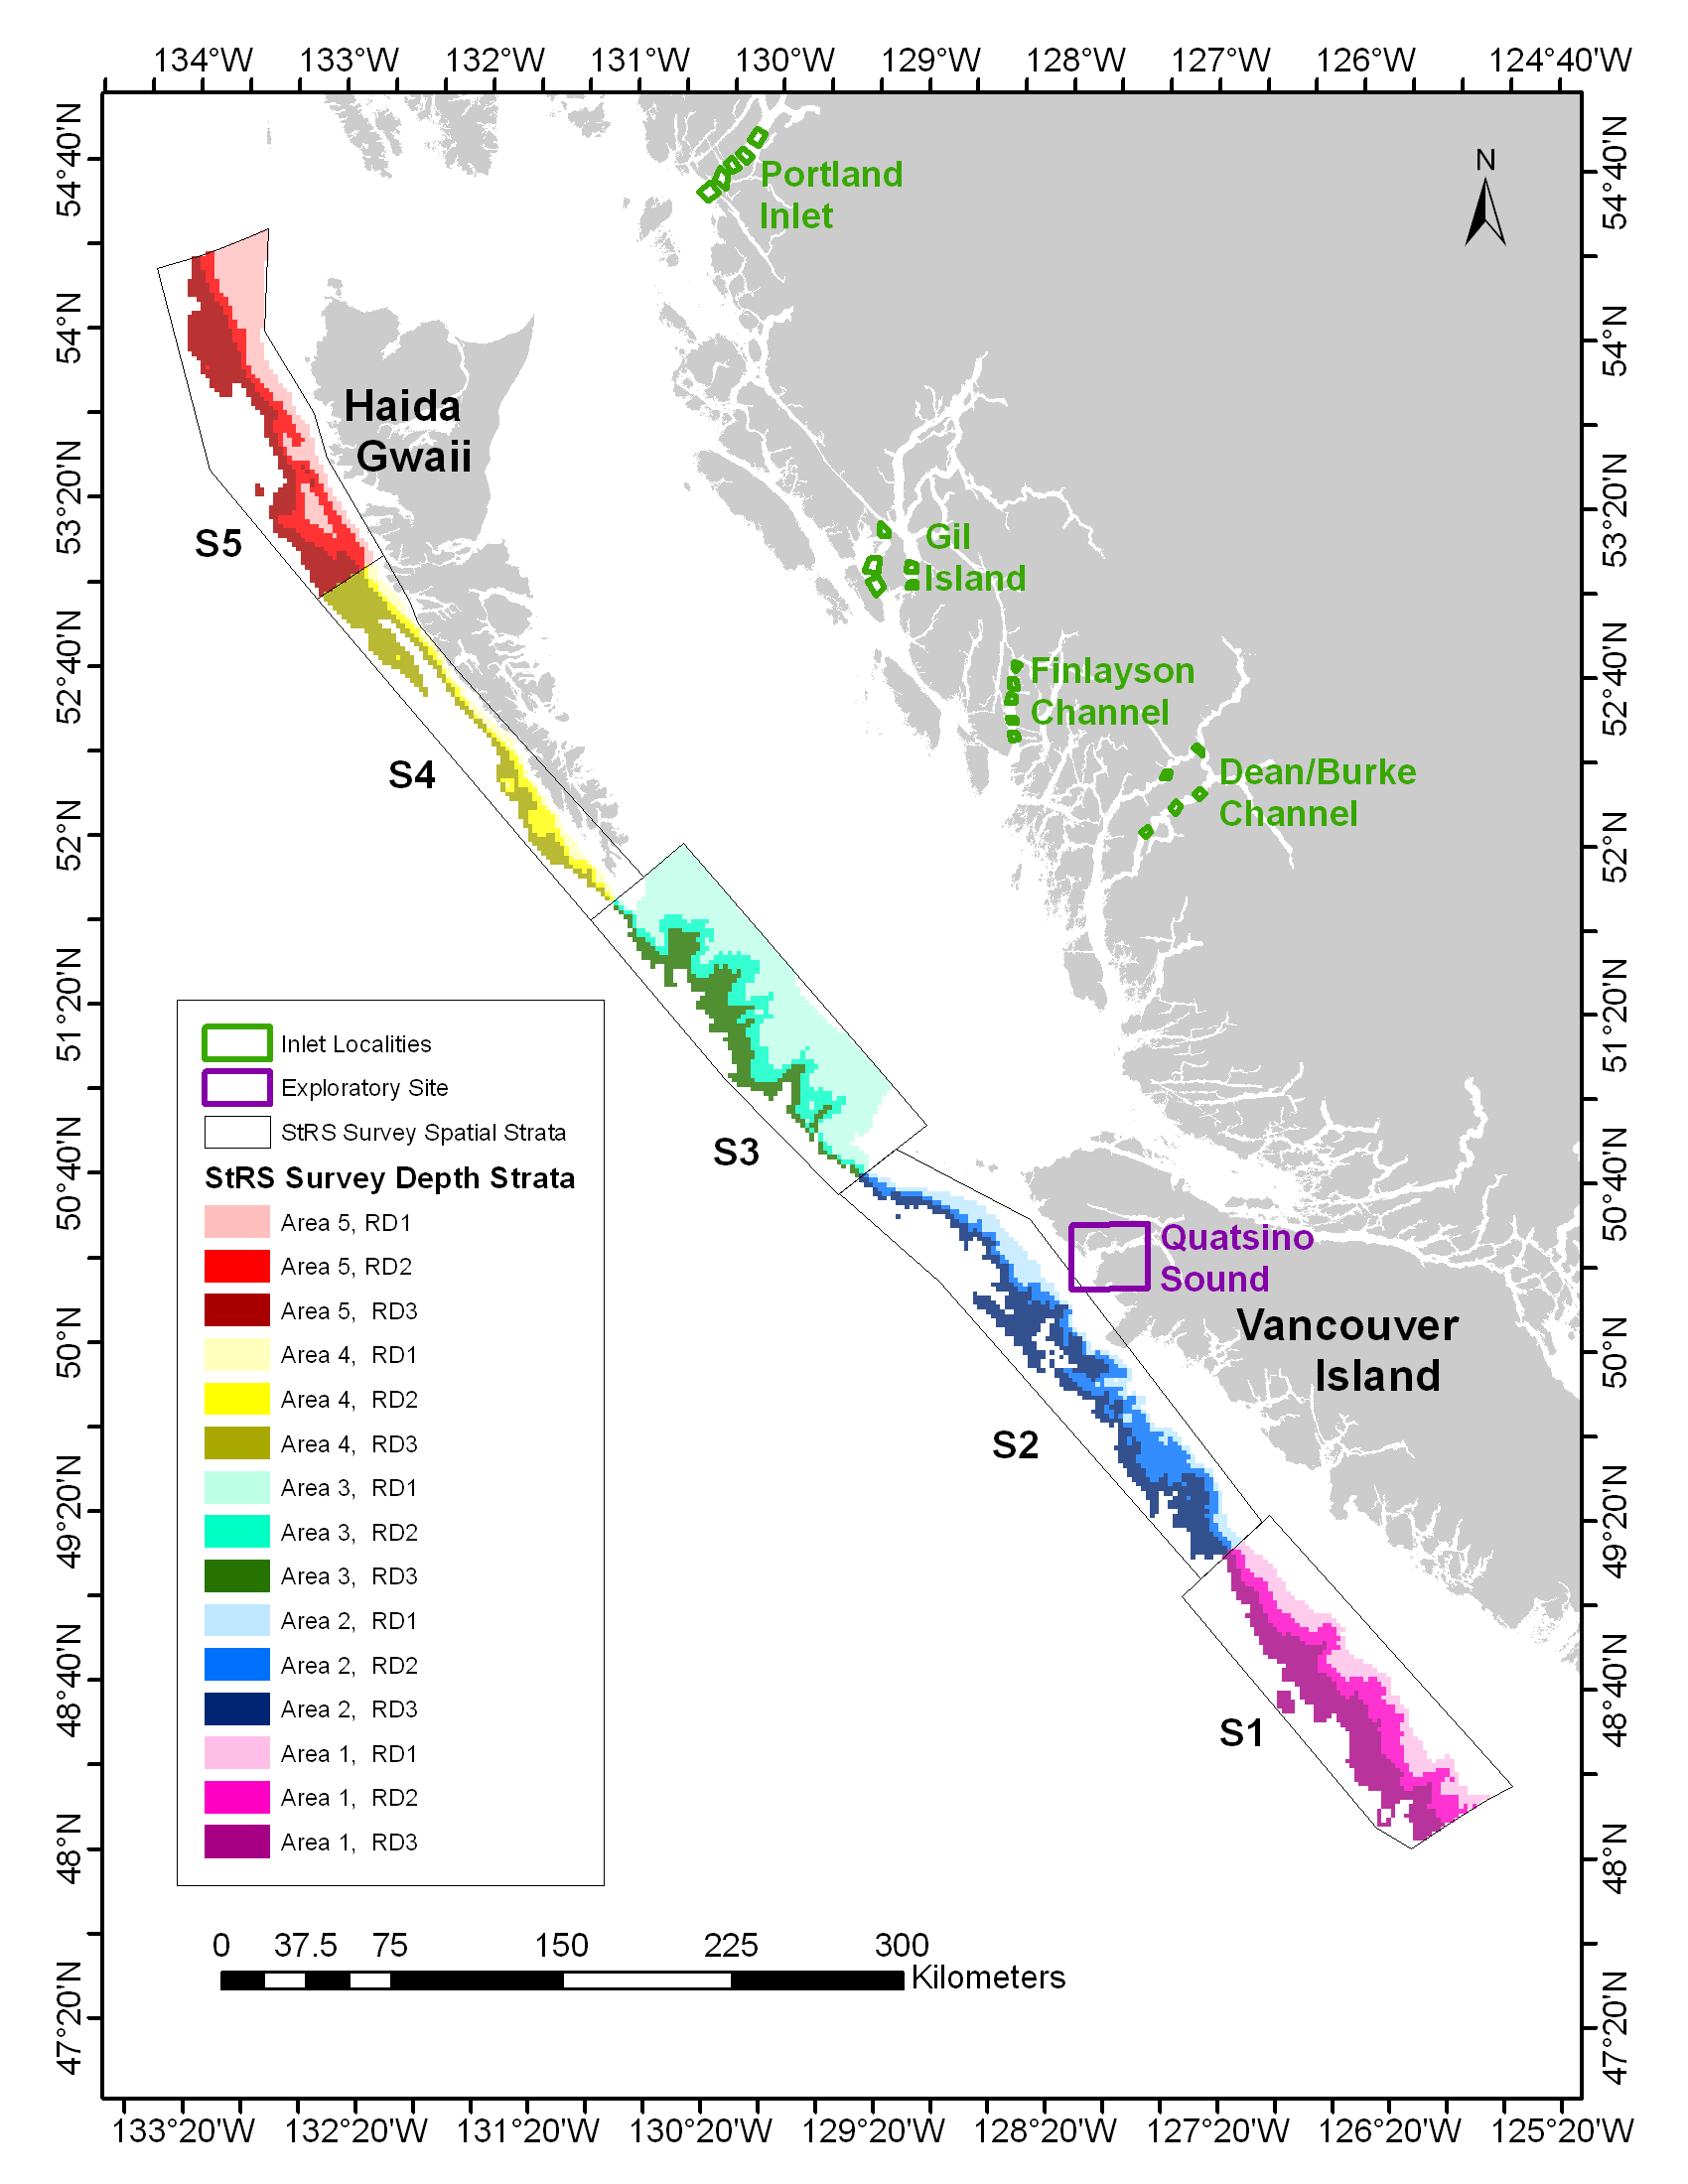
\includegraphics[width=410px]{c:/github/surveyreport_2012/figures/figure1}}{Figure \ref{fig:figure1}} 

}

\caption{Location of the boundaries of the mainland inlet localities, one exploratory site and the five spatial areas (S\textsubscript{1}-S\textsubscript{5}) of the stratified random survey design. The three depths strata (RD\textsubscript{1}-RD\textsubscript{3}) are colour-coded and nested within each of the five spatial strata.}\label{fig:figure1}
\end{figure}
\clearpage


\begin{figure}[htb]

{\centering \pdftooltip{\includegraphics[width=480px,height=381px]{c:/github/surveyreport_2012/figures/figure2}}{Figure \ref{fig:figure2}} 

}

\caption{Start locations of survey sets in 2012 conducted in the stratified random survey areas S\textsubscript{1} through S\textsubscript{5} (red markers) and in the exploratory area (purple markers). The camera sets are represented by yellow markers.}\label{fig:figure2}
\end{figure}
\clearpage


\begin{figure}[htb]

{\centering \pdftooltip{\includegraphics[width=480px,height=360px]{c:/github/surveyreport_2012/figures/figure3}}{Figure \ref{fig:figure3}} 

}

\caption{Image of the F/V Ocean Pearl used for the 2012 sablefish research and assessment survey. Photo credit: .}\label{fig:figure3}
\end{figure}
\clearpage


\begin{figure}[htb]

{\centering \pdftooltip{\includegraphics[width=370px,height=610px]{c:/github/surveyreport_2012/figures/figure4}}{Figure \ref{fig:figure4}} 

}

\caption{Trap elements (A). Trap gear elements consisting of 25 baited traps snapped to beckets along a groundline (B).}\label{fig:figure4}
\end{figure}
\clearpage


\begin{figure}[htb]

{\centering \pdftooltip{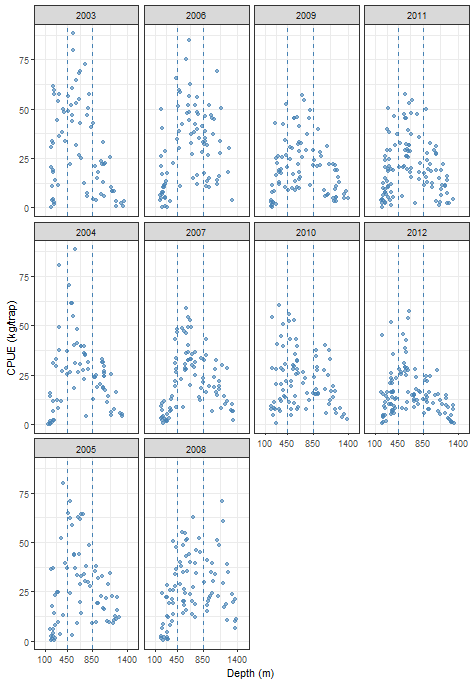
\includegraphics[width=400px]{c:/github/surveyreport_2012/figures/figure5}}{Figure \ref{fig:figure5}} 

}

\caption{Sablefish catch per unit effort (CPUE) by depth and year for StRS sets. Dashed lines delineate depth strata (shallow(RD\textsubscript{1}) = 100-450m, mid(RD\textsubscript{2}) = 450-850m, deep(RD\textsubscript{3}) = 850-1400m).}\label{fig:figure5}
\end{figure}
\clearpage


\begin{figure}[htb]

{\centering \pdftooltip{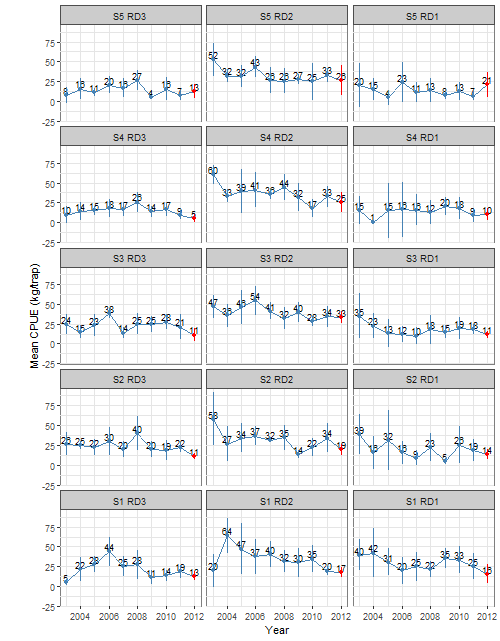
\includegraphics[width=450px,height=576px]{c:/github/surveyreport_2012/figures/figure6}}{Figure \ref{fig:figure6}} 

}

\caption{Average Sablefish catch per unit effort (CPUE; mean +/- 95\% CIs) by survey strata since 2003. Panels run deep to shallow (left to right) and north to south (top to bottom).}\label{fig:figure6}
\end{figure}
\clearpage


\begin{figure}[htb]

{\centering \pdftooltip{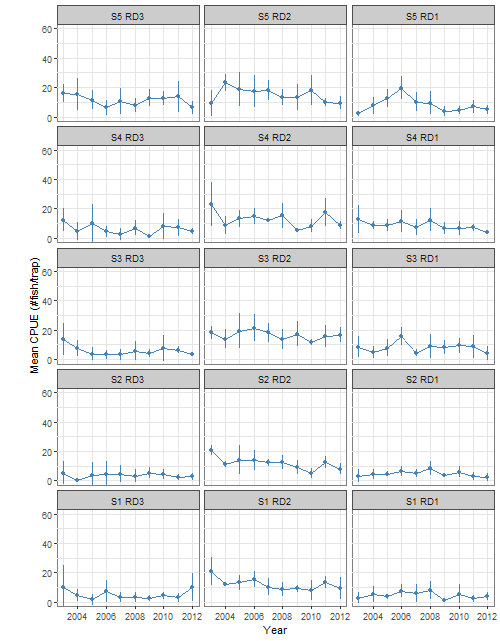
\includegraphics[width=450px,height=576px]{c:/github/surveyreport_2012/figures/figure7}}{Figure \ref{fig:figure7}} 

}

\caption{Average number of sablefish per trap (mean +/- 95\% CIs) by StRS survey strata over time. Panels run shallow to deep (left to right) and south to north (top to bottom).}\label{fig:figure7}
\end{figure}
\clearpage


\begin{figure}[htb]

{\centering \pdftooltip{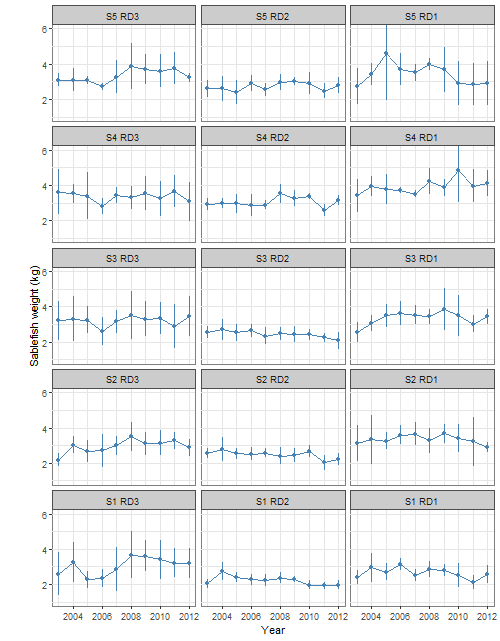
\includegraphics[width=450px,height=576px]{c:/github/surveyreport_2012/figures/figure8}}{Figure \ref{fig:figure8}} 

}

\caption{Average weight of sablefish (mean +/- 95\% CIs) by survey strata over time. Panels run shallow to deep (left to right) and south to north (top to bottom).}\label{fig:figure8}
\end{figure}
\clearpage


\begin{figure}[htb]

{\centering \pdftooltip{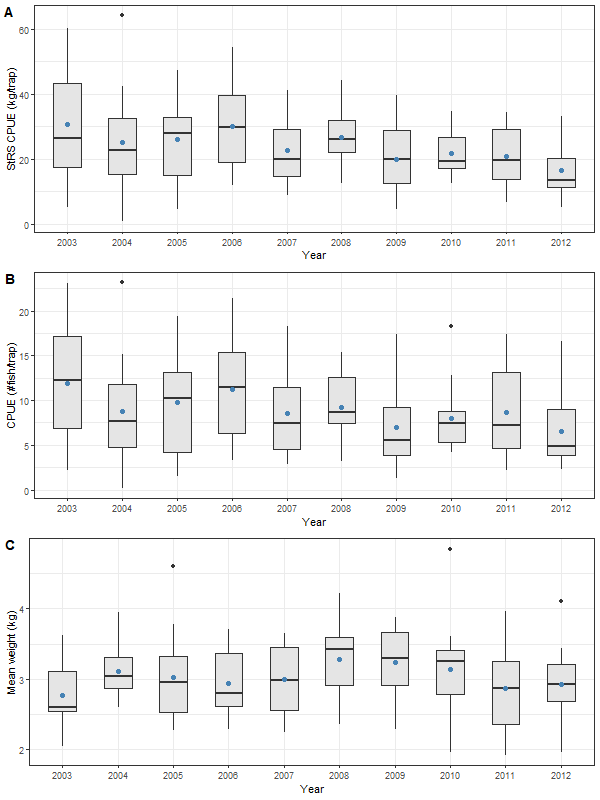
\includegraphics[width=450px,height=576px]{c:/github/surveyreport_2012/figures/figure9}}{Figure \ref{fig:figure9}} 

}

\caption{Annual mean weight of sablefish per trap (kg/trap) (A); annual mean number of sablefish per trap (\#fish/trap) (B); annual mean weight of sablefish (kg) (C) by StRS survey strata over time. Horizontal line is median and blue dots are arithmetic mean.}\label{fig:figure9}
\end{figure}
\clearpage


\begin{figure}[htb]

{\centering \pdftooltip{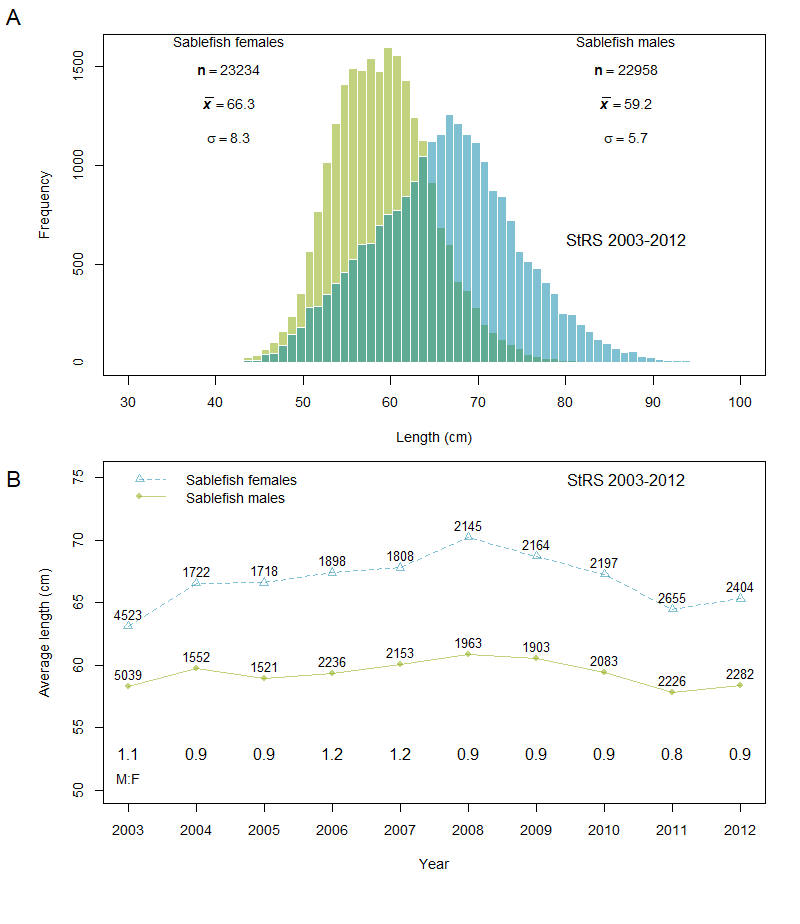
\includegraphics[width=450px,height=550px]{c:/github/surveyreport_2012/figures/figure10}}{Figure \ref{fig:figure10}} 

}

\caption{Length frequencies for female (cyan) and male sablefish (green) and up to 2013 for all StRS sets. The number of specimens is denoted by the letter n, the mean indicated by the xbar \(\overline{x}\) and the standard deviation is represented by the symbol sigma \(\Sigma\) (A). Average length and ratios of male and female sablefish by year. Counts by sex are shown across the top of the lines (B).}\label{fig:figure10}
\end{figure}
\clearpage


\begin{figure}[htb]

{\centering \pdftooltip{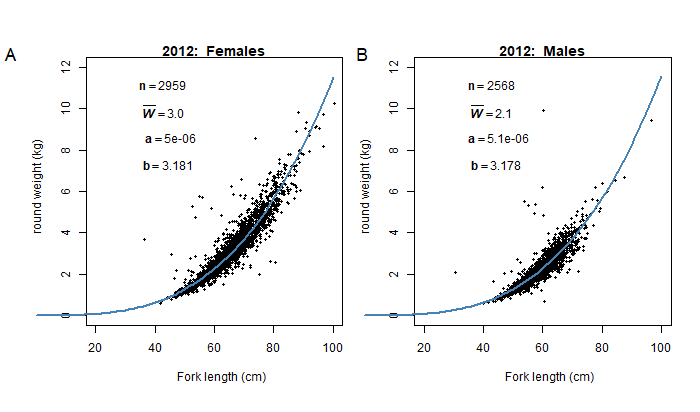
\includegraphics[width=480px,height=282px]{c:/github/surveyreport_2012/figures/figure11}}{Figure \ref{fig:figure11}} 

}

\caption{Sablefish fork length (L in cm) vs weight (W in kg) for females (A) and males (B) for the 2012 survey.}\label{fig:figure11}
\end{figure}

\begin{figure}[htb]

{\centering \pdftooltip{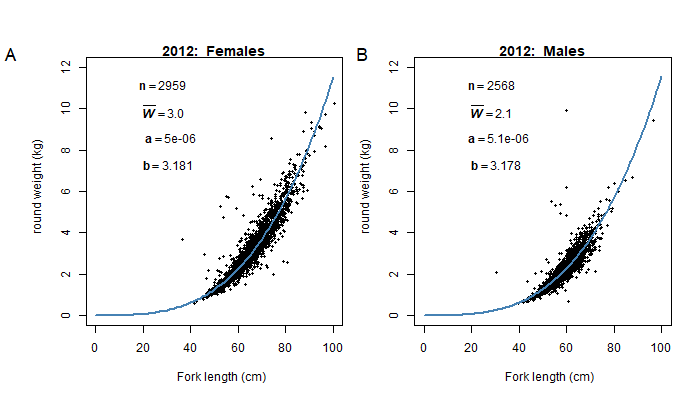
\includegraphics[width=500px,height=577px]{c:/github/surveyreport_2012/figures/figure12}}{Figure \ref{fig:figure12}} 

}

\caption{Bubble plot for female (A) and male (B) sablefish ages by survey year from StRS sets that have been aged. The sizes of the circles are proportional to the number of fish with given ages. Fish age 35 and older are included in one bubble. The total number(n) of fish aged are listed across the top of each panel. The ages with the highest ratios are posted to the right of each bubble.}\label{fig:figure12}
\end{figure}
\clearpage


\begin{figure}[htb]

{\centering \pdftooltip{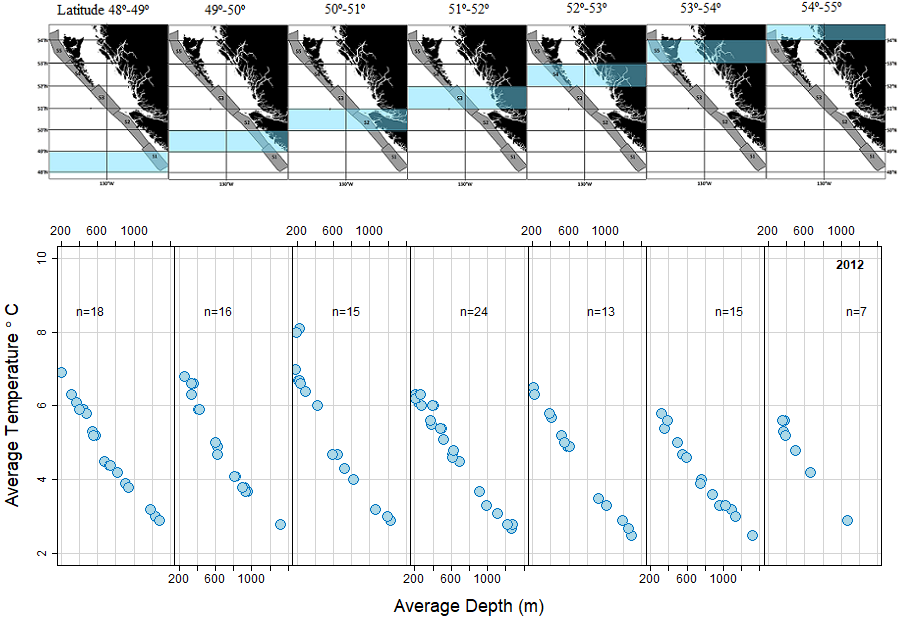
\includegraphics[width=500px,height=335px]{c:/github/surveyreport_2012/figures/figure13}}{Figure \ref{fig:figure13}} 

}

\caption{Coplot of average depth (m) vs average temperature (\(^\circ\)C) for a given 1-degree latitude range (blue bands) for 2012. The number of fishing sets deployed with a SBE 39 recorder are represented by n.}\label{fig:figure13}
\end{figure}
\clearpage


\begin{figure}[htb]

{\centering \pdftooltip{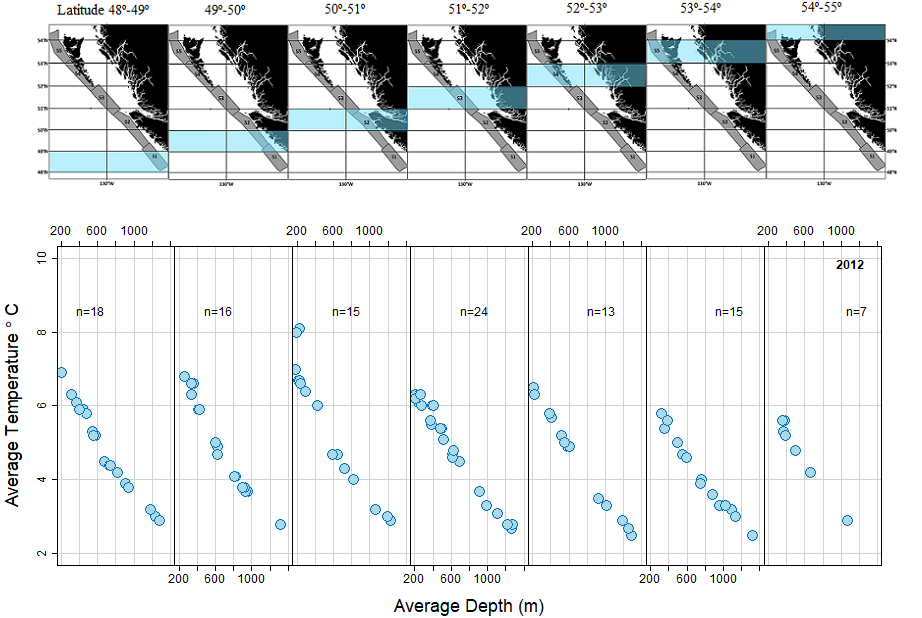
\includegraphics[width=440px,height=540px]{c:/github/surveyreport_2012/figures/figure14}}{Figure \ref{fig:figure14}} 

}

\caption{Vertical density ridgeplots of mean temperatures per year as reported by set from the Sea-bird SBE 39 loggers on traps at three depth intervals, RD\textsubscript{1} = shallow (100-450 m), RD\textsubscript{2} = mid (450-850 m), RD\textsubscript{3} = deep (850-1400 m). Lines indicate the 2.5\% and 97.5\% tails.}\label{fig:figure14}
\end{figure}
\clearpage

\clearpage


\begin{figure}[htb]

{\centering \pdftooltip{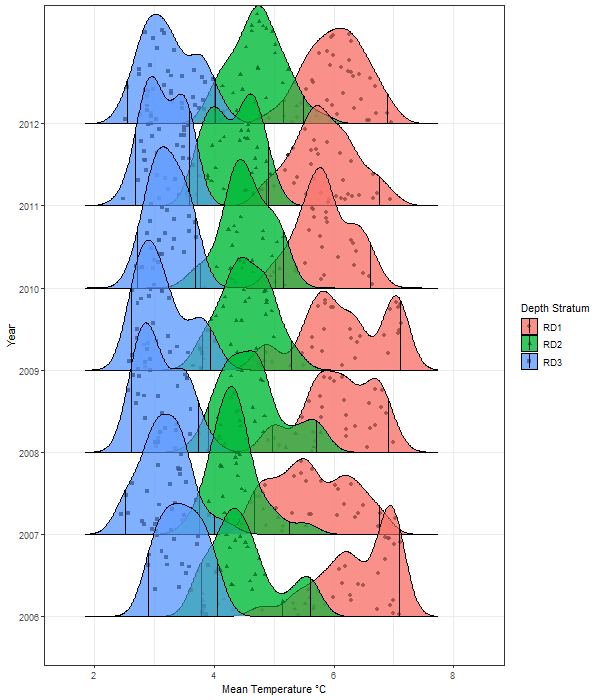
\includegraphics[width=450px,height=582px]{c:/github/surveyreport_2012/figures/figure15}}{Figure \ref{fig:figure15}} 

}

\caption{Location of the epicentre of a 7.7 magnitude earthquake on Saturday October 27, 2012 at 8:04 p.m. The accelerometer on the ocean floor captured the earthquake event (inset).}\label{fig:figure15}
\end{figure}
\clearpage

\begin{appendices}
\counterwithin{figure}{section}
\counterwithin{table}{section}
\counterwithin{equation}{section}

\clearpage

\section{LIST OF SABLEFISH RESEARCH AND ASSESSMENT SURVEYS.}
\label{app:first-appendix}

\begingroup\fontsize{8}{10}\selectfont
\begin{longtable}{rlllrr}
\toprule
\textbf{Year} & \textbf{Dates} & \textbf{Vessel} & \textbf{Captain} & \textbf{Set Count} & \textbf{GFBIO Id}\\
\midrule
1988 & Oct 28  - Nov 24 & VICIOUS FISHER & VANCE FLETCHER & 16 & 43990\\
1989 & Oct 19  - Nov 18 & LA PORSCHE & SIGURD BRYNJOLFSON & 29 & 43910\\
1990 & Nov  8  - Nov 18 & VIKING STAR & DOUG FARRINGTON & 24 & 43750\\
1991 & Oct  9  - Oct 29 & W. E. RICKER & ALAN FARRINGTON & 32 & 43673\\
1992 & Oct 13  - Nov  4 & W. E. RICKER & RON ROBERTS & 38 & 43670\\
1993 & Oct 19  - Nov 11 & W. E. RICKER & ALAN FARRINGTON & 42 & 43650\\
1994 & Oct 13  - Oct 31 & LA PORSCHE & RICHARD BEAUVAIS & 39 & 43630\\
1994 & Oct 18  - Nov 13 & WESTERN VIKING & RICK JONES & 27 & 43390\\
1995 & Oct  8  - Oct 20 & OCEAN PEARL & ROBERT FRAUMENI & 29 & 43270\\
1995 & Oct 11  - Oct 28 & VICTOR F & MICHAEL DERRY & 34 & 43330\\
1995 & Oct  1  - Oct 31 & VIKING SUNRISE & JASON OLSEN & 40 & 43350\\
1996 & Sep 26  - Oct 10 & OCEAN PEARL & MICHAEL DERRY & 32 & 43039\\
1996 & Sep 30  - Oct 22 & VIKING STAR & OTTO ELVAN & 49 & 43210\\
1996 & May 10  - May 30 & VIKING SUNRISE & ALBERT (DEACON) MELNYCHUK & 42 & 43024\\
1997 & Sep 26  - Oct 21 & OCEAN PEARL & MICHAEL DERRY & 74 & 42699\\
1997 & May 20  - Jun 10 & VIKING SUNRISE & ALBERT (DEACON) MELNYCHUK & 42 & 42760\\
1998 & Sep 22  - Oct 17 & OCEAN PEARL & MICHAEL DERRY & 89 & 41122\\
1999 & Sep 29  - Oct 30 & OCEAN PEARL & MICHAEL DERRY & 109 & 40589\\
2000 & Oct  8  - Nov 14 & PACIFIC VIKING & ALBERT (DEACON) MELNYCHUK & 131 & 40517\\
2001 & Oct  6  - Nov  6 & OCEAN PEARL & MICHAEL DERRY & 134 & 43233\\
2002 & Oct  4  - Nov  7 & PACIFIC VIKING & ALBERT (DEACON) MELNYCHUK & 125 & 48120\\
2002 & Oct  5  - Nov 13 & VIKING SUNRISE & JASON OLSEN & 90 & 48110\\
2003 & Oct 15  - Nov 13 & OCEAN PEARL & MICHAEL DERRY & 94 & 52100\\
2003 & Oct  7  - Nov 10 & VIKING STAR & JIM FARRINGTON & 84 & 52120\\
2004 & Oct  5  - Nov 15 & MILBANKE SOUND & DON QUAST & 95 & 58145\\
2004 & Oct  5  - Nov  3 & OCEAN MARAUDER & ALBERT (DEACON) MELNYCHUK & 84 & 57360\\
2005 & Oct  4  - Nov  2 & PACIFIC VIKING & ALBERT (DEACON) MELNYCHUK & 84 & 60529\\
2005 & Oct  7  - Nov 17 & VIKING SUNRISE & RORY JOHNSON & 88 & 60503\\
2006 & Oct  1  - Nov  1 & PACIFIC VIKING & ALBERT (DEACON) MELNYCHUK & 98 & 62966\\
2006 & Oct  2  - Nov 15 & SENA II & TIM JOYS & 98 & 62666\\
2007 & Oct  7  - Nov 12 & PACIFIC VIKING & ALBERT (DEACON) MELNYCHUK & 99 & 65106\\
2007 & Oct  8  - Nov 12 & VIKING TIDE & JASON OLSEN & 91 & 65107\\
2008 & Sep 29  - Nov 16 & OCEAN PEARL & ROBERT FRAUMENI & 157 & 67007\\
2009 & Oct  8  - Nov 25 & OCEAN PEARL & ROBERT FRAUMENI & 155 & 69067\\
2010 & Oct  9  - Nov 30 & OCEAN PEARL & ROBERT FRAUMENI & 153 & 70787\\
2011 & Oct  9  - Nov 21 & OCEAN PEARL & DARCY NICHOLS & 132 & 72067\\
2012 & Oct  9  - Nov 17 & OCEAN PEARL & DARCY NICHOLS & 135 & 73190\\
\bottomrule
\end{longtable}
\endgroup{}

\clearpage

\section{DATA FORMS 2012 SABLEFISH SURVEY.}
\label{app:second-appendix}
\begin{center}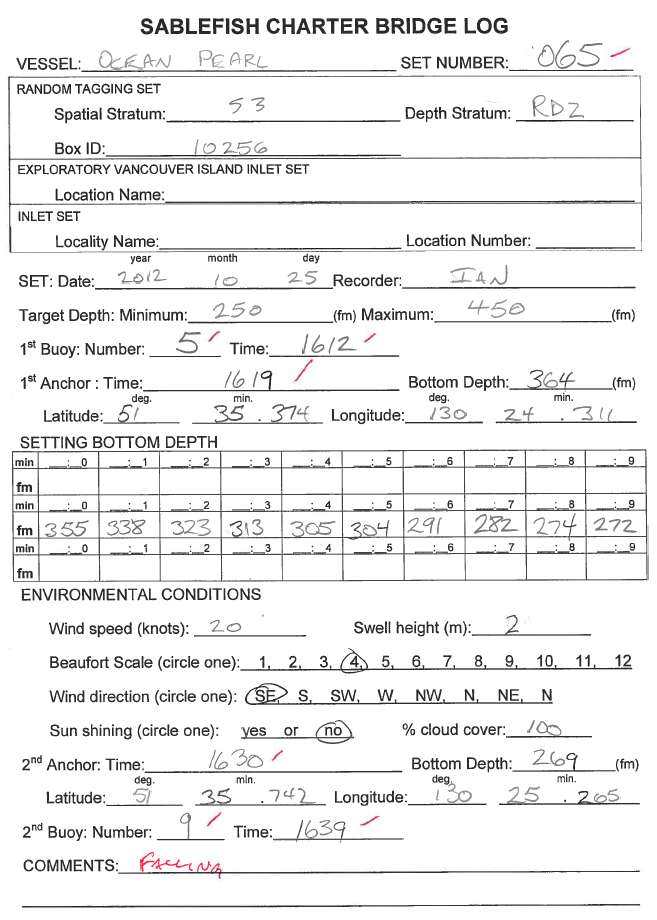
\includegraphics[width=370px,height=518px]{c:/github/surveyreport_2012/figures/AppendixC1_BridgeLog} \end{center}

Figure B.1. Example of a completed bridge log data form used during the 2012 survey. This form was completed from the bridge of the Ocean Pearl for each set.

\clearpage
\begin{center}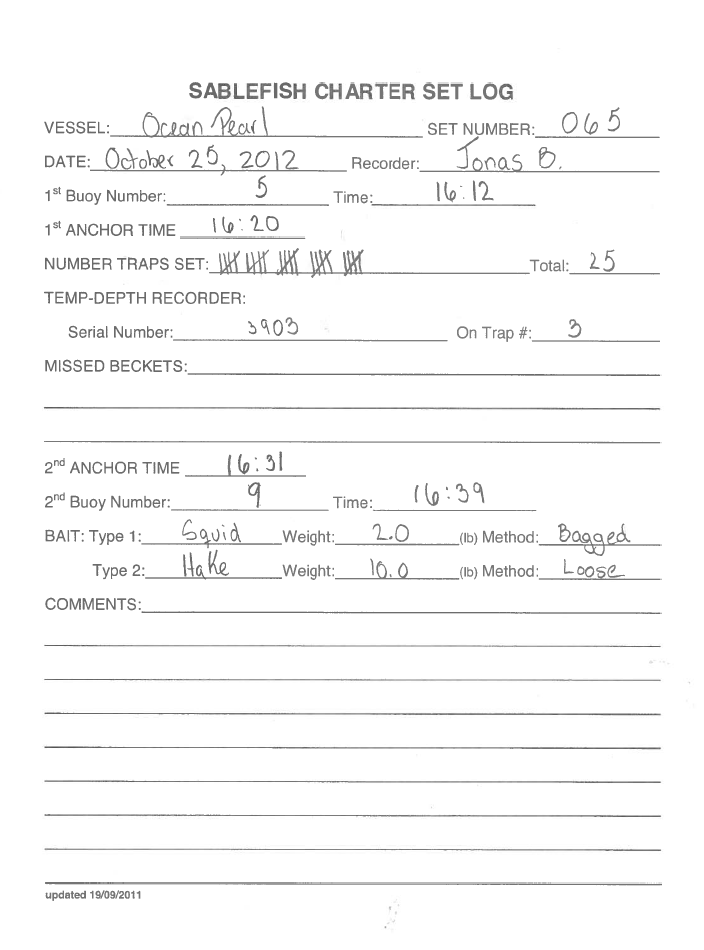
\includegraphics[width=400px,height=539px]{c:/github/surveyreport_2012/figures/AppendixC2_SetLog} \end{center}

Figure B.2. Example of a completed set log data form used during the 2012 survey. This from was completed by science staff from the deck as the gear was set.

\clearpage
\begin{center}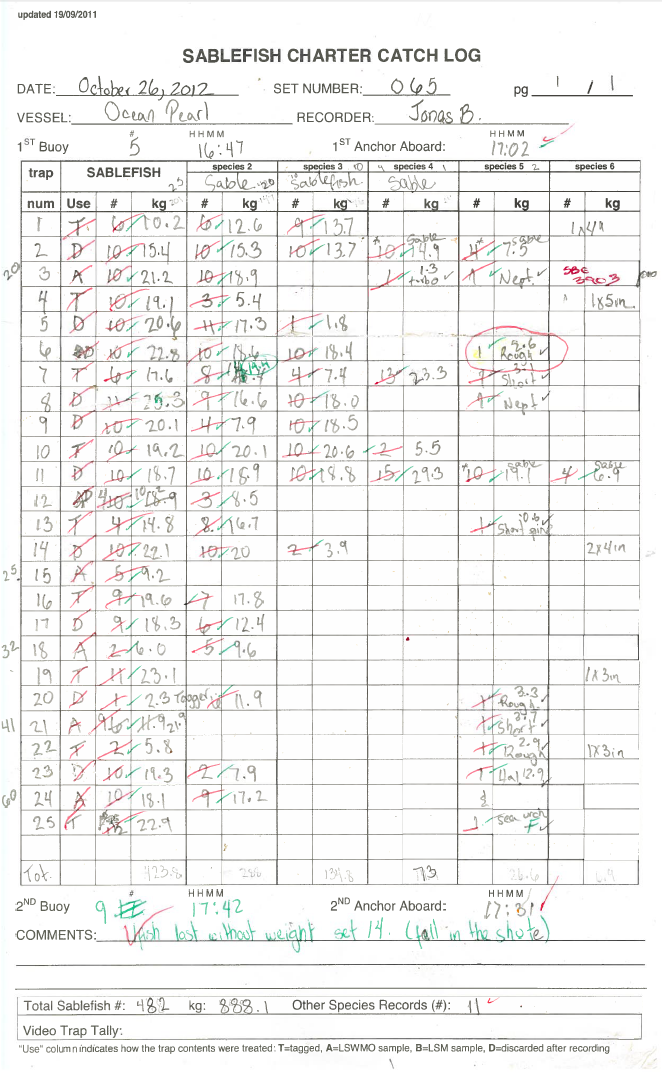
\includegraphics[width=370px,height=599px]{c:/github/surveyreport_2012/figures/AppendixC3_CatchLog} \end{center}

Figure B.3. Example of a completed catch log data form. \clearpage
\begin{center}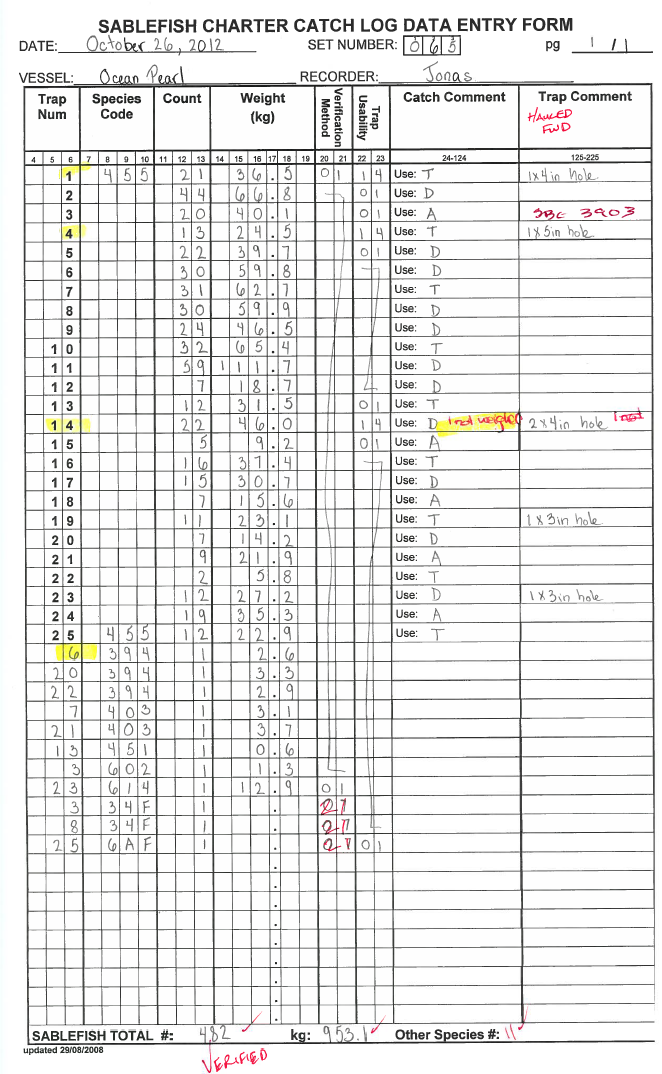
\includegraphics[width=370px,height=600px]{c:/github/surveyreport_2012/figures/AppendixC4_CatchLogTab} \end{center}

Figure B.4. Example of a tabular catch log data entry form transposed from the catch log in Figure C.3.

\clearpage
\begin{center}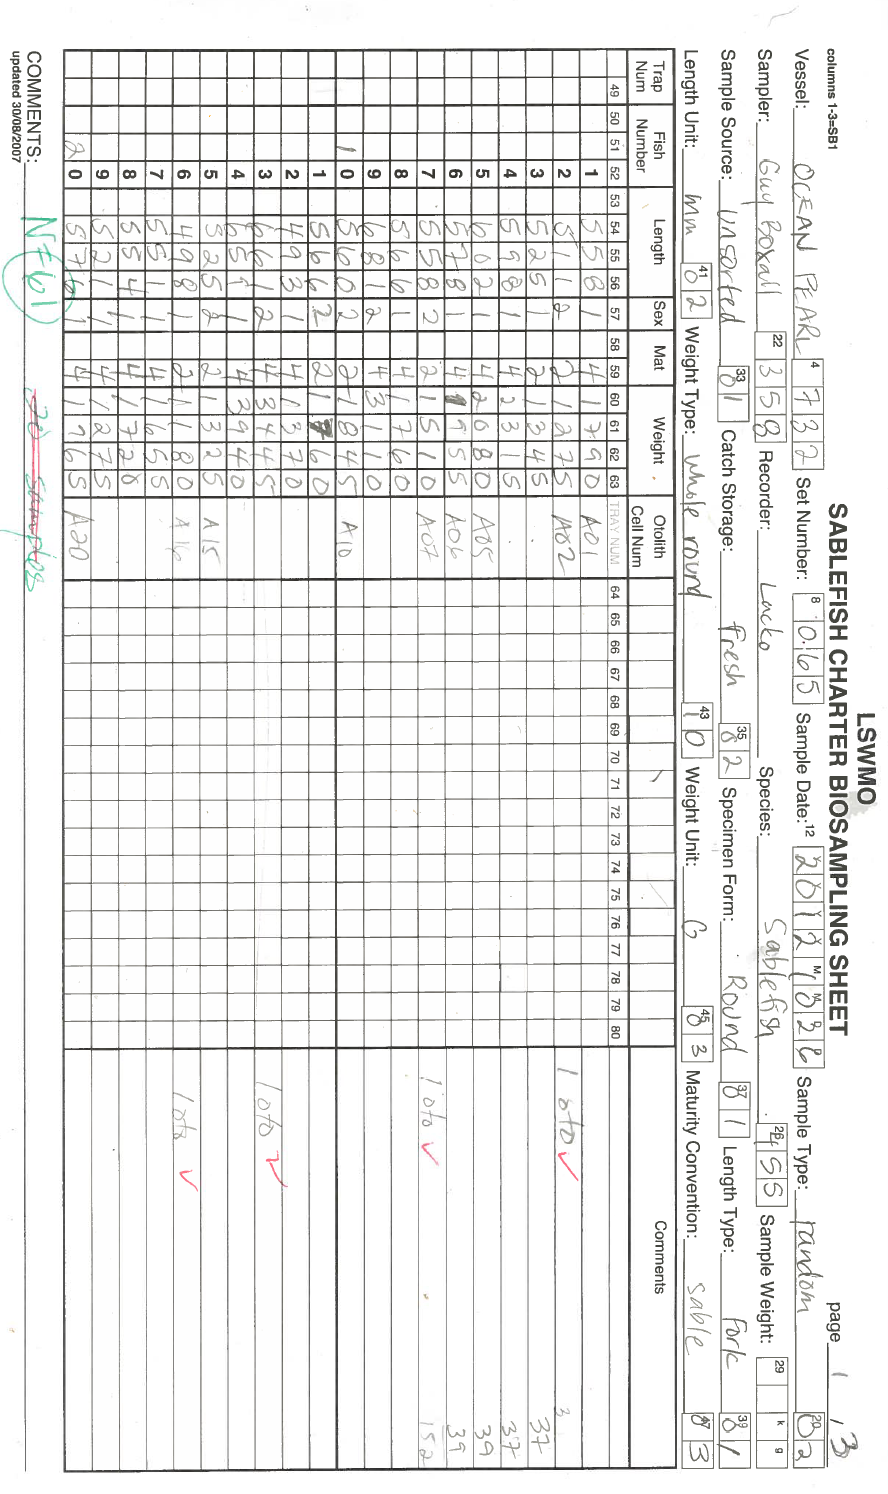
\includegraphics[width=350px,height=588px]{c:/github/surveyreport_2012/figures/AppendixC5_LSWMO} \end{center}

Figure B.5. Example of a completed biological sampling form.

\clearpage
\begin{center}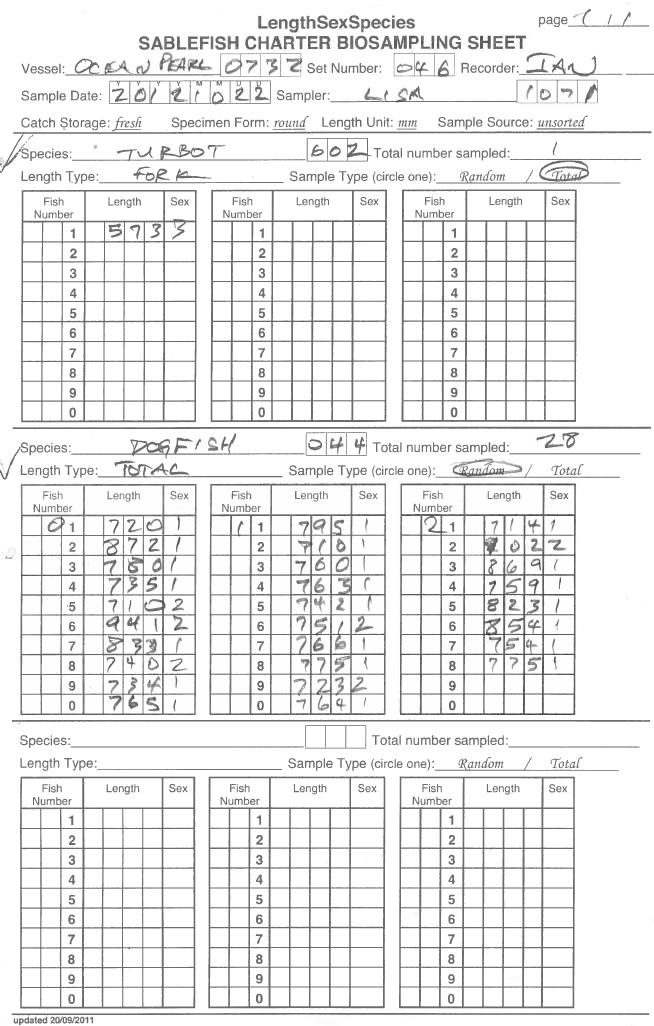
\includegraphics[width=370px,height=580px]{c:/github/surveyreport_2012/figures/AppendixC6_LengthSexSpecies} \end{center}

Figure B.6. Example of a completed LSS biological sampling form used during the 2012 survey for samples of species other than sablefish or rougheye/blackspotted rockfish.

\clearpage
\begin{flushleft}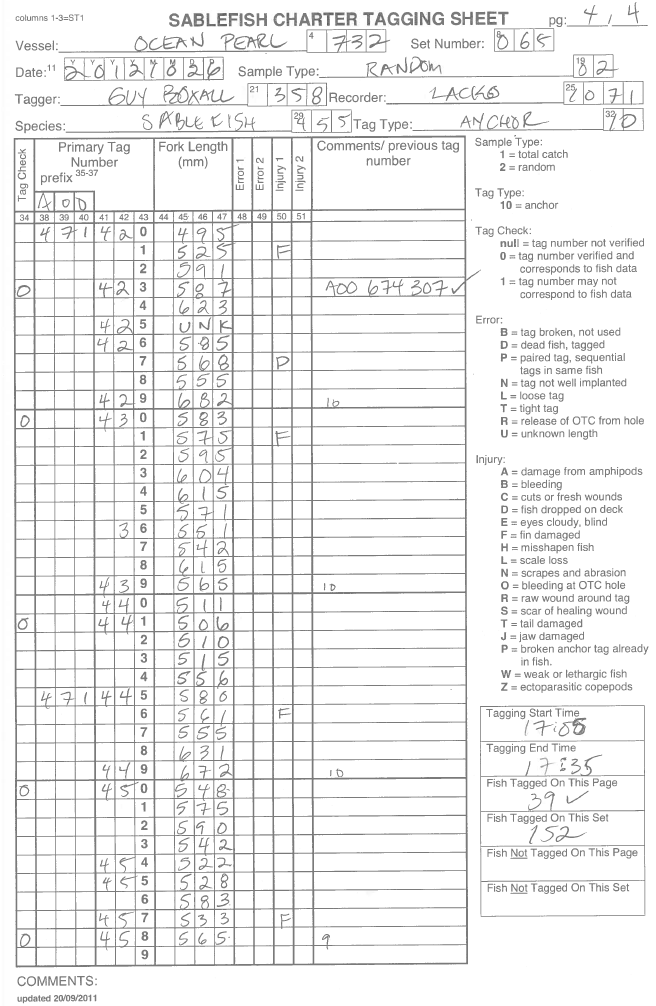
\includegraphics[width=390px,height=613px]{c:/github/surveyreport_2012/figures/AppendixC7_TaggingSheet} \end{flushleft}

Figure B.7. Example of a completed tagging form used during the 2012 survey.

\clearpage
\begin{flushleft}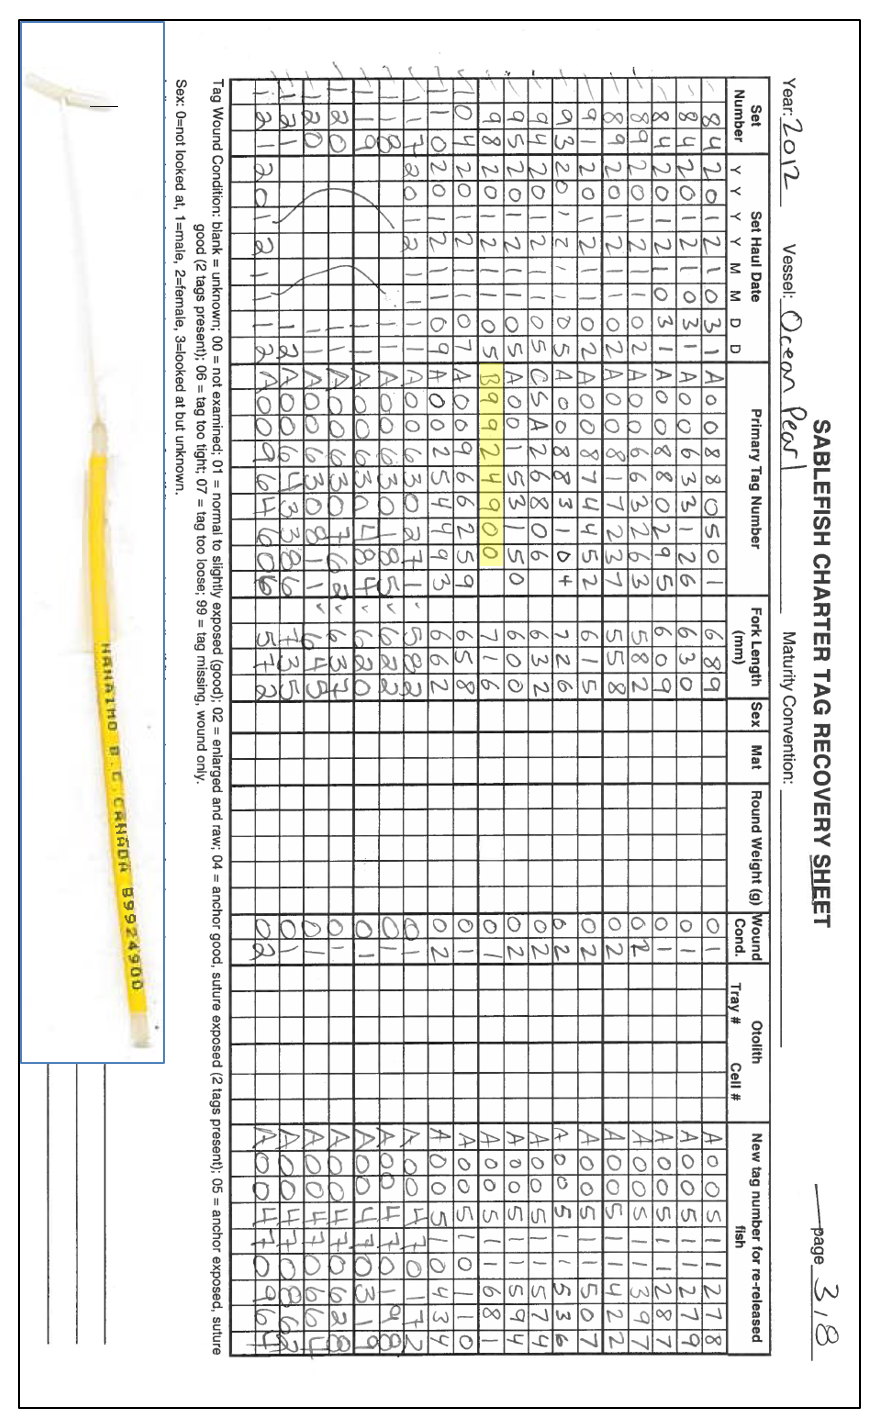
\includegraphics[width=370px,height=600px]{c:/github/surveyreport_2012/figures/AppendixC8_tagRecovery} \end{flushleft}

Figure B.8. Example of a completed tag recovery form used during the 2012 survey. Image of recovered tag B9924900 (inset)

\clearpage

\section{SET DETAILS 2012.}
\label{app:third-appendix}

Details of sets completed during the 2012 survey program (F/V Ocean Pearl). Sets are listed by stratum/inlet name, set type, depth stratum, start date, end of gear deployment time and duration in minutes. The depth strata for type 3 tagging sets include RD\textsubscript{1} (100-250 fathoms), RD\textsubscript{2} (250-450 fathoms) and RD\textsubscript{3} (450-750 fathoms). The position data includes the major area and start and end latitude and longitude in degrees decimal minutes. The bottom depths (in meters) of the fishing set are shown with the mean bottom depth calculated from recordings at one minute intervals between the start and end of the set. The number of traps fished for each set excludes open traps, while holed or fouled traps have been included. Sets that successfully deployed a Seabird SBE temperature and pressure recorder or Hobo accelerometer or Nuytco autonomous camera system are indicated with an `x'.
\begin{landscape}\begingroup\fontsize{8}{10}\selectfont
\begin{longtable}{>{\centering\arraybackslash}p{1.5cm}>{\centering\arraybackslash}p{0.7cm}>{\centering\arraybackslash}p{0.7cm}>{\centering\arraybackslash}p{0.7cm}>{\centering\arraybackslash}p{0.9cm}>{\centering\arraybackslash}p{0.6cm}>{\centering\arraybackslash}p{0.9cm}>{\centering\arraybackslash}p{0.5cm}>{\centering\arraybackslash}p{1.2cm}>{\centering\arraybackslash}p{1.7cm}>{\centering\arraybackslash}p{1.2cm}>{\centering\arraybackslash}p{1.7cm}>{\centering\arraybackslash}p{0.7cm}>{\centering\arraybackslash}p{0.7cm}>{\centering\arraybackslash}p{0.5cm}>{\centering\arraybackslash}p{0.6cm}>{\centering\arraybackslash}p{0.4cm}>{\centering\arraybackslash}p{0.3cm}>{\centering\arraybackslash}p{0.3cm}}
\toprule
\textbf{Spatial Stratum} & \textbf{Set} & \textbf{Type} & \textbf{Depth Stratum} & \textbf{Date} & \textbf{Time} & \textbf{Duration (minutes)} & \textbf{Area} & \textbf{Start Latitude} & \textbf{Start Longitude} & \textbf{End Latitude} & \textbf{End Longitude} & \textbf{Start Depth (m)} & \textbf{End Depth (m)} & \textbf{Mean Depth (m)} & \textbf{Traps Fished} & \textbf{SBE 39} & \textbf{Hobo} & \textbf{Cam}\\
\midrule
\endfirsthead
\multicolumn{19}{@{}l}{continued.}\\
\toprule
\textbf{Spatial Stratum} & \textbf{Set} & \textbf{Type} & \textbf{Depth Stratum} & \textbf{Date} & \textbf{Time} & \textbf{Duration (minutes)} & \textbf{Area} & \textbf{Start Latitude} & \textbf{Start Longitude} & \textbf{End Latitude} & \textbf{End Longitude} & \textbf{Start Depth (m)} & \textbf{End Depth (m)} & \textbf{Mean Depth (m)} & \textbf{Traps Fished} & \textbf{SBE 39} & \textbf{Hobo} & \textbf{Cam}\\
\midrule
\endhead

\endfoot
\bottomrule
\endlastfoot
S1 & 1 & StRS & RD3 & Oct 10 & 11:56 & 1326 & 3C & 48° 0.4'N & 126° 4.7'W & 48° 1.1'N & 126° 4.7'W & 949 & 949 & 952 & 25 & x &  & \\
S1 & 2 & StRS & RD2 & Oct 10 & 13:55 & 1409 & 3C & 48° 5.3'N & 125° 59.8'W & 48° 4.6'N & 125° 59.8'W & 799 & 759 & 802 & 25 & x &  & \\
S1 & 3 & StRS & RD2 & Oct 10 & 15:55 & 1408 & 3C & 48° 0.8'N & 126° 0.5'W & 48° 0.5'N & 125° 59.6'W & 669 & 784 & 751 & 25 & x & x & \\
S1 & 4 & StRS & RD3 & Oct 10 & 18:02 & 1466 & 3C & 48° 3.2'N & 126° 18.8'W & 48° 2.7'N & 126° 19.4'W & 1185 & 1207 & 1199 & 25 & x &  & \\
S1 & 5 & StRS & RD3 & Oct 10 & 19:55 & 1484 & 3C & 48° 9.2'N & 126° 21.7'W & 48° 9.2'N & 126° 20.9'W & 1203 & 1223 & 1212 & 25 & x &  & \\
 & 6 & camera &  & Oct 11 & 08:47 & 211 & 3C & 48° 4.6'N & 125° 58.1'W & 48° 4.9'N & 125° 57.3'W & 570 & 556 & 563 & 0 & x & x & x\\
 & 7 & camera &  & Oct 12 & 06:54 & 538 & 3C & 48° 0.1'N & 126° 18.6'W & 48° 0.1'N & 126° 19.5'W & 391 & 442 & 409 & 0 & x & x & x\\
S1 & 8 & StRS & RD2 & Oct 12 & 07:45 & 1346 & 3C & 48° 9.6'N & 126° 22.8'W & 48° 9.5'N & 126° 23.7'W & 705 & 733 & 711 & 25 & x &  & \\
S1 & 9 & StRS & RD3 & Oct 12 & 09:38 & 1351 & 3C & 48° 4.9'N & 126° 22.8'W & 48° 5'N & 126° 21.8'W & 923 & 837 & 877 & 25 & x &  & \\
S1 & 10 & StRS & RD2 & Oct 12 & 11:39 & 1329 & 3C & 48° 4.7'N & 126° 17.6'W & 48° 5.1'N & 126° 16.8'W & 782 & 673 & 715 & 25 & x &  & \\
S1 & 11 & StRS & RD1 & Oct 12 & 13:14 & 1318 & 3C & 48° 8.7'N & 126° 14.3'W & 48° 8.9'N & 126° 13.3'W & 455 & 334 & 407 & 26 & x &  & \\
S1 & 12 & StRS & RD2 & Oct 12 & 15:08 & 1303 & 3C & 48° 1.6'N & 126° 16.7'W & 48° 1.6'N & 126° 17.8'W & 464 & 603 & 517 & 25 & x &  & \\
S1 & 13 & StRS & RD2 & Oct 12 & 17:03 & 1326 & 3C & 48° 2.8'N & 126° 24.5'W & 48° 2.8'N & 126° 25.5'W & 532 & 623 & 572 & 25 & x &  & \\
S1 & 14 & StRS & RD1 & Oct 12 & 18:41 & 1315 & 3C & 48° 6.5'N & 126° 27.5'W & 48° 6.5'N & 126° 28.4'W & 312 & 303 & 307 & 25 & x & x & \\
S1 & 15 & StRS & RD1 & Oct 12 & 20:21 & 1304 & 3C & 48° 9.8'N & 126° 28.8'W & 48° 9.8'N & 126° 29.8'W & 199 & 203 & 203 & 24 & x &  & \\
S1 & 16 & StRS & RD1 & Oct 12 & 21:33 & 1347 & 3C & 48° 5.3'N & 126° 32.3'W & 48° 5.5'N & 126° 33.3'W & 354 & 438 & 409 & 25 & x &  & \\
S1 & 17 & StRS & RD3 & Oct 14 & 08:18 & 1324 & 3C & 48° 1.5'N & 126° 52'W & 48° 2.1'N & 126° 52.1'W & 1293 & 1327 & 1316 & 25 & x &  & \\
S1 & 18 & StRS & RD3 & Oct 14 & 10:11 & 1358 & 3C & 48° 9'N & 126° 46.8'W & 48° 9.6'N & 126° 46.9'W & 1212 & 1201 & 1212 & 25 & x &  & \\
S1 & 19 & StRS & RD3 & Oct 14 & 11:53 & 1358 & 3C & 48° 3.2'N & 126° 45'W & 48° 3.2'N & 126° 46.1'W & 830 & 883 & 855 & 25 & x &  & \\
S1 & 20 & StRS & RD2 & Oct 14 & 13:51 & 1323 & 3C & 48° 5.3'N & 126° 43.4'W & 48° 5.3'N & 126° 44.6'W & 548 & 640 & 592 & 25 & x &  & \\
S1 & 21 & StRS & RD2 & Oct 14 & 15:41 & 1356 & 3C & 48° 5'N & 126° 35.1'W & 48° 5'N & 126° 36.1'W & 676 & 824 & 737 & 25 & x & x & \\
S1 & 22 & StRS & RD1 & Oct 14 & 17:32 & 1342 & 3C & 48° 7.6'N & 126° 40.2'W & 48° 8.1'N & 126° 41.2'W & 378 & 365 & 371 & 25 & x &  & \\
S1 & 23 & StRS & RD1 & Oct 14 & 18:59 & 1362 & 3D & 49° 0.5'N & 126° 49.6'W & 49° 0.5'N & 126° 50.7'W & 329 & 367 & 345 & 25 & x &  & \\
S1 & 24 & StRS & RD3 & Oct 14 & 21:11 & 1403 & 3D & 49° 0.1'N & 127° 4'W & 49° 0.1'N & 127° 3'W & 1283 & 1300 & 1322 & 25 & x &  & \\
S1 & 25 & StRS & RD1 & Oct 16 & 08:03 & 1318 & 3D & 49° 4.4'N & 127° 5.8'W & 49° 4.6'N & 127° 4.4'W & 429 & 287 & 371 & 25 & x &  & \\
 & 26 & camera &  & Oct 16 & 09:09 & 1324 & 3D & 49° 7.1'N & 127° 8.5'W & 49° 7'N & 127° 7.9'W & 274 & 252 & 265 & 0 & x &  & x\\
S2 & 27 & StRS & RD1 & Oct 16 & 10:27 & 1328 & 3D & 49° 1.1'N & 127° 14.5'W & 49° 1.5'N & 127° 13.6'W & 453 & 285 & 367 & 25 & x &  & \\
S2 & 28 & StRS & RD3 & Oct 16 & 11:54 & 1363 & 3D & 49° 1.3'N & 127° 19.2'W & 49° 1.7'N & 127° 18.5'W & 961 & 832 & 896 & 25 & x &  & \\
S2 & 29 & StRS & RD1 & Oct 16 & 13:48 & 1349 & 3D & 49° 5.6'N & 127° 14.9'W & 49° 5.6'N & 127° 13.8'W & 371 & 197 & 250 & 25 & x &  & \\
S2 & 30 & StRS & RD1 & Oct 16 & 15:33 & 1320 & 3D & 49° 8.7'N & 127° 14.8'W & 49° 8.7'N & 127° 13.7'W & 376 & 190 & 267 & 25 & x &  & \\
S2 & 31 & StRS & RD2 & Oct 16 & 17:42 & 1322 & 3D & 49° 5.4'N & 127° 25.9'W & 49° 5.9'N & 127° 25.2'W & 769 & 656 & 705 & 25 & x & x & \\
S2 & 32 & StRS & RD2 & Oct 16 & 19:22 & 1339 & 3D & 49° 8.9'N & 127° 34'W & 49° 8.4'N & 127° 33.4'W & 618 & 791 & 704 & 25 & x &  & \\
S2 & 33 & StRS & RD3 & Oct 16 & 21:11 & 1355 & 3D & 49° 1.4'N & 127° 43.9'W & 49° 1'N & 127° 43.4'W & 916 & 852 & 872 & 25 & x & x & \\
S2 & 34 & StRS & RD3 & Oct 18 & 08:24 & 1322 & 3D & 49° 4.8'N & 127° 49.4'W & 49° 5.4'N & 127° 49.3'W & 1018 & 905 & 923 & 25 & x &  & \\
S2 & 35 & StRS & RD2 & Oct 18 & 10:13 & 1336 & 3D & 49° 0.2'N & 127° 48.6'W & 49° 0.3'N & 127° 47.9'W & 709 & 656 & 711 & 25 & x &  & \\
S2 & 36 & StRS & RD1 & Oct 18 & 12:04 & 1321 & 3D & 49° 4.3'N & 127° 50.1'W & 49° 4.4'N & 127° 49.3'W & 451 & 367 & 398 & 25 & x &  & \\
S2 & 37 & StRS & RD3 & Oct 18 & 14:18 & 1335 & 3D & 49° 6.6'N & 128° 7'W & 49° 6.9'N & 128° 6'W & 960 & 823 & 919 & 25 & x &  & \\
S2 & 38 & StRS & RD2 & Oct 18 & 15:55 & 1331 & 3D & 49° 8.2'N & 128° 6.7'W & 49° 8.5'N & 128° 5.9'W & 810 & 704 & 733 & 25 & x & x & \\
S2 & 39 & StRS & RD3 & Oct 18 & 17:43 & 1345 & 3D & 50° 0.2'N & 128° 3.9'W & 50° 0.2'N & 128° 5.2'W & 1234 & 1347 & 1254 & 25 & x &  & \\
S2 & 40 & StRS & RD3 & Oct 18 & 19:35 & 1365 & 3D & 50° 0.4'N & 128° 8.8'W & 50° 0.1'N & 128° 9.7'W & 857 & 1135 & 1044 & 25 & x &  & \\
S2 & 41 & StRS & RD2 & Oct 18 & 21:38 & 1382 & 3D & 50° 0.4'N & 127° 57.4'W & 50° 0'N & 127° 58.4'W & 601 & 479 & 546 & 25 & x &  & \\
 & 42 & explore &  & Oct 20 & 01:03 & 2709 & 3D & 50° 7.9'N & 127° 57.2'W & 50° 8.2'N & 127° 56.4'W & 214 & 230 & 226 & 26 & x &  & \\
 & 43 & explore &  & Oct 20 & 01:42 & 2617 & 3D & 50° 8.3'N & 127° 55'W & 50° 8.2'N & 127° 53.9'W & 206 & 208 & 214 & 25 & x &  & \\
S2 & 44 & StRS & RD3 & Oct 21 & 08:16 & 1337 & 3D & 50° 2.4'N & 128° 12.2'W & 50° 2.4'N & 128° 13.3'W & 1018 & 1346 & 1210 & 25 & x &  & \\
S2 & 45 & StRS & RD2 & Oct 21 & 10:02 & 1343 & 3D & 50° 7.7'N & 128° 15.5'W & 50° 7.8'N & 128° 16.7'W & 475 & 515 & 566 & 25 & x &  & \\
S2 & 46 & StRS & RD1 & Oct 21 & 11:55 & 1327 & 3D & 50° 5.1'N & 128° 18.7'W & 50° 4.2'N & 128° 19.7'W & 186 & 192 & 188 & 25 & x &  & \\
S2 & 47 & StRS & RD3 & Oct 21 & 14:20 & 1308 & 3D & 50° 4.2'N & 128° 30.7'W & 50° 4.8'N & 128° 31.3'W & 865 & 824 & 919 & 25 & x & x & \\
S2 & 48 & StRS & RD2 & Oct 21 & 16:07 & 1330 & 5A & 50° 2.4'N & 128° 39'W & 50° 2.5'N & 128° 40.2'W & 515 & 698 & 669 & 24 & x &  & \\
S2 & 49 & StRS & RD1 & Oct 21 & 18:00 & 1358 & 5A & 50° 0.4'N & 128° 54.1'W & 50° 0.5'N & 128° 55.2'W & 223 & 239 & 226 & 25 & x &  & \\
S2 & 50 & StRS & RD1 & Oct 21 & 19:33 & 1350 & 5A & 50° 2.1'N & 129° 1.2'W & 50° 2.1'N & 129° 2.2'W & 466 & 384 & 334 & 25 & x &  & \\
S3 & 51 & StRS & RD1 & Oct 23 & 07:40 & 1349 & 5A & 50° 1.2'N & 129° 28.2'W & 50° 1.2'N & 129° 29.4'W & 217 & 223 & 219 & 25 & x &  & \\
S3 & 52 & StRS & RD2 & Oct 23 & 09:02 & 1384 & 5A & 50° 2.2'N & 129° 37.7'W & 50° 2.7'N & 129° 38.4'W & 623 & 557 & 508 & 25 & x &  & \\
S3 & 53 & StRS & RD1 & Oct 23 & 10:39 & 1371 & 5A & 50° 4.7'N & 129° 35.8'W & 50° 5.3'N & 129° 36.4'W & 232 & 239 & 237 & 25 & x &  & \\
S3 & 54 & StRS & RD1 & Oct 23 & 11:58 & 1389 & 5A & 50° 9.6'N & 129° 36.8'W & 50° 9.6'N & 129° 38'W & 268 & 358 & 343 & 25 & x &  & \\
S3 & 55 & StRS & RD3 & Oct 23 & 14:11 & 1433 & 5A & 51° 0.5'N & 129° 59.4'W & 51° 0.9'N & 130° 0.2'W & 905 & 863 & 896 & 25 & x & x & \\
S3 & 56 & StRS & RD3 & Oct 23 & 16:08 & 1442 & 5A & 51° 0.9'N & 130° 9.6'W & 51° 0.9'N & 130° 10.8'W & 1247 & 1243 & 1241 & 25 & x &  & \\
S3 & 57 & StRS & RD2 & Oct 23 & 18:07 & 1463 & 5B & 51° 6'N & 130° 4.8'W & 51° 6.7'N & 130° 5.1'W & 684 & 539 & 587 & 25 & x &  & \\
S3 & 58 & StRS & RD1 & Oct 23 & 19:53 & 1487 & 5A & 51° 3.6'N & 129° 52.5'W & 51° 4.1'N & 129° 53.3'W & 460 & 289 & 347 & 25 & x &  & \\
S3 & 59 & StRS & RD1 & Oct 23 & 21:53 & 1478 & 5A & 51° 4.8'N & 129° 39.1'W & 51° 4.8'N & 129° 40.4'W & 261 & 256 & 256 & 25 & x &  & \\
S3 & 60 & StRS & RD1 & Oct 25 & 07:33 & 1347 & 5B & 51° 0'N & 129° 57.7'W & 51° 0.5'N & 129° 56.7'W & 257 & 248 & 254 & 25 & x &  & \\
S3 & 61 & StRS & RD2 & Oct 25 & 09:03 & 1385 & 5B & 51° 9.3'N & 130° 6.4'W & 51° 9.5'N & 130° 7.3'W & 556 & 689 & 620 & 25 & x &  & \\
S3 & 62 & StRS & RD2 & Oct 25 & 11:05 & 1412 & 5B & 51° 8.9'N & 130° 15.4'W & 51° 8.9'N & 130° 16.7'W & 680 & 760 & 727 & 25 & x &  & \\
S3 & 63 & StRS & RD3 & Oct 25 & 12:36 & 1439 & 5B & 51° 0.7'N & 130° 17.2'W & 51° 0.7'N & 130° 18.3'W & 1075 & 1144 & 1119 & 25 & x &  & \\
S3 & 64 & StRS & RD3 & Oct 25 & 14:41 & 1456 & 5B & 51° 8.6'N & 130° 23.9'W & 51° 8.6'N & 130° 25.1'W & 1276 & 1338 & 1289 & 25 & x &  & \\
S3 & 65 & StRS & RD2 & Oct 25 & 16:19 & 1483 & 5B & 51° 5.4'N & 130° 24.3'W & 51° 5.7'N & 130° 25.3'W & 665 & 491 & 559 & 25 & x &  & \\
S3 & 66 & StRS & RD2 & Oct 25 & 18:05 & 1474 & 5B & 51° 7'N & 130° 17.5'W & 51° 7'N & 130° 18.6'W & 603 & 491 & 577 & 25 & x & x & \\
S3 & 67 & StRS & RD1 & Oct 25 & 19:51 & 1475 & 5B & 51° 9.2'N & 130° 20.8'W & 51° 9.8'N & 130° 21.3'W & 426 & 294 & 353 & 25 & x &  & \\
S3 & 68 & StRS & RD1 & Oct 25 & 21:33 & 1501 & 5B & 51° 0.5'N & 130° 12'W & 51° 0.6'N & 130° 10.8'W & 274 & 299 & 287 & 25 & x &  & \\
S3 & 69 & StRS & RD1 & Oct 27 & 07:31 & 1352 & 5B & 51° 1.3'N & 130° 15.9'W & 51° 1.3'N & 130° 17.1'W & 204 & 210 & 208 & 25 & x &  & \\
S3 & 70 & StRS & RD1 & Oct 27 & 09:00 & 1356 & 5B & 51° 4.9'N & 130° 14'W & 51° 5'N & 130° 15.1'W & 226 & 230 & 226 & 25 & x &  & \\
S3 & 71 & StRS & RD1 & Oct 27 & 10:32 & 1334 & 5B & 51° 4.6'N & 130° 19.7'W & 51° 4.7'N & 130° 20.7'W & 245 & 312 & 270 & 25 & x & x & \\
S3 & 72 & StRS & RD3 & Oct 27 & 12:57 & 1368 & 5B & 51° 6.8'N & 130° 32.9'W & 51° 6.8'N & 130° 34.1'W & 1294 & 1307 & 1298 & 25 & x &  & \\
S3 & 73 & StRS & RD3 & Oct 27 & 15:13 & 1400 & 5B & 51° 9.9'N & 130° 50.4'W & 51° 9.9'N & 130° 51.5'W & 903 & 982 & 941 & 25 & x &  & \\
S3 & 74 & StRS & RD1 & Oct 27 & 17:03 & 1420 & 5B & 51° 7.4'N & 130° 42.2'W & 51° 7.2'N & 130° 43.6'W & 453 & 373 & 422 & 25 & x &  & \\
S3 & 75 & StRS & RD1 & Oct 27 & 18:48 & 1432 & 5B & 51° 2.3'N & 130° 38.7'W & 51° 2.2'N & 130° 39.9'W & 369 & 327 & 356 & 25 & x &  & \\
S3 & 76 & StRS & RD1 & Oct 27 & 20:40 & 1444 & 5B & 51° 9.7'N & 130° 37.8'W & 52° 0.4'N & 130° 33.1'W & 400 & 336 & 367 & 25 & x &  & \\
S4 & 77 & StRS & RD1 & Oct 30 & 07:59 & 1335 & 5B & 51° 3.2'N & 131° 2.1'W & 51° 2.6'N & 131° 2.5'W & 182 & 250 & 226 & 25 & x &  & \\
S4 & 78 & StRS & RD2 & Oct 30 & 09:35 & 1345 & 5B & 51° 4.2'N & 131° 5.1'W & 51° 3.7'N & 131° 5.7'W &  & 667 & 541 & 25 & x &  & \\
S4 & 79 & StRS & RD2 & Oct 30 & 11:34 & 1354 & 5B & 51° 9.8'N & 131° 13.9'W & 51° 9.7'N & 131° 14.8'W & 501 & 572 & 620 & 25 & x &  & \\
S4 & 80 & StRS & RD1 & Oct 30 & 12:58 & 1347 & 5E & 52° 0.6'N & 131° 15.7'W & 52° 0.6'N & 131° 17.2'W & 221 & 226 & 224 & 25 & x & x & \\
S4 & 81 & StRS & RD2 & Oct 30 & 14:33 & 1338 & 5E & 52° 0'N & 131° 20.2'W & 52° 0.5'N & 131° 20.8'W & 468 & 486 & 504 & 25 & x &  & \\
S4 & 82 & StRS & RD2 & Oct 30 & 16:32 & 1336 & 5E & 52° 0.1'N & 131° 31.4'W & 52° 0'N & 131° 30.3'W & 466 & 720 & 594 & 25 & x &  & \\
S4 & 83 & StRS & RD2 & Oct 30 & 18:35 & 1335 & 5E & 52° 6.2'N & 131° 32.8'W & 52° 6.6'N & 131° 33.7'W & 471 & 640 & 563 & 25 & x &  & \\
S4 & 84 & StRS & RD2 & Oct 30 & 20:22 & 1326 & 5E & 52° 0.5'N & 131° 38.7'W & 52° 1'N & 131° 39.5'W & 497 & 640 & 581 & 25 & x &  & \\
S4 & 85 & StRS & RD1 & Nov  1 & 08:00 & 1356 & 5E & 52° 8.4'N & 131° 45.2'W & 52° 8.5'N & 131° 46.9'W & 192 & 468 & 301 & 25 & x &  & \\
S4 & 86 & StRS & RD1 & Nov  1 & 09:36 & 1360 & 5E & 52° 1.5'N & 131° 51.5'W & 52° 2.1'N & 131° 52.3'W & 360 & 257 & 353 & 25 & x &  & \\
S4 & 87 & StRS & RD1 & Nov  1 & 11:05 & 1386 & 5E & 52° 7.8'N & 132° 2.5'W & 52° 8.3'N & 132° 3.4'W & 294 & 431 & 426 & 25 & x &  & \\
S4 & 88 & StRS & RD3 & Nov  1 & 13:06 & 1399 & 5E & 52° 2.9'N & 132° 10.7'W & 52° 2.9'N & 132° 11.9'W & 1029 & 1377 & 1236 & 25 & x &  & \\
S4 & 89 & StRS & RD3 & Nov  1 & 15:07 & 1406 & 5E & 52° 3.5'N & 132° 22.1'W & 52° 3.5'N & 132° 23.4'W & 969 & 896 & 901 & 25 & x &  & \\
S4 & 90 & StRS & RD3 & Nov  1 & 17:11 & 1394 & 5E & 52° 4.5'N & 132° 26.9'W & 52° 4.5'N & 132° 28.1'W & 1221 & 1357 & 1287 & 25 & x & x & \\
S4 & 91 & StRS & RD3 & Nov  1 & 18:45 & 1453 & 5E & 52° 7.9'N & 132° 27.9'W & 52° 7.9'N & 132° 29.1'W & 976 & 914 & 940 & 25 & x &  & \\
S4 & 92 & StRS & RD3 & Nov  1 & 20:27 & 1526 & 5E & 52° 6.1'N & 132° 41'W & 52° 6.1'N & 132° 42.3'W & 1309 & 1293 & 1303 & 25 & x &  & \\
S4 & 93 & StRS & RD1 & Nov  3 & 08:14 & 2957 & 5E & 53° 0'N & 132° 32.5'W & 53° 0'N & 132° 33.6'W & 305 & 354 & 369 & 24 & x &  & \\
S4 & 94 & StRS & RD3 & Nov  3 & 09:50 & 3025 & 5E & 53° 0.6'N & 132° 45'W & 53° 0.6'N & 132° 46.1'W & 1011 & 1121 & 1082 & 25 & x &  & \\
S5 & 95 & StRS & RD3 & Nov  3 & 11:39 & 3099 & 5E & 53° 0.1'N & 132° 55.8'W & 53° 0.1'N & 132° 56.8'W & 1108 & 1111 & 1111 & 25 & x &  & \\
S5 & 96 & StRS & RD3 & Nov  3 & 13:39 & 3140 & 5E & 53° 0'N & 133° 2.8'W & 53° 0'N & 133° 4'W & 1342 & 1342 & 1344 & 25 & x &  & \\
S5 & 97 & StRS & RD2 & Nov  3 & 15:36 & 3165 & 5E & 53° 3.7'N & 133° 3.6'W & 53° 3.6'N & 133° 4.8'W & 780 & 766 & 769 & 25 & x & x & \\
S5 & 98 & StRS & RD1 & Nov  3 & 17:18 & 3157 & 5E & 53° 8.9'N & 133° 5.9'W & 53° 8.9'N & 133° 7.1'W & 347 & 448 & 400 & 25 & x &  & \\
S5 & 99 & StRS & RD2 & Nov  3 & 18:47 & 3216 & 5E & 53° 5.4'N & 133° 10.4'W & 53° 5.4'N & 133° 11.5'W & 460 & 693 & 585 & 25 & x &  & \\
S5 & 100 & StRS & RD3 & Nov  3 & 20:31 & 3238 & 5E & 53° 0.5'N & 133° 9.4'W & 53° 0.5'N & 133° 10.6'W & 806 & 951 & 1005 & 24 & x &  & \\
S5 & 101 & StRS & RD1 & Nov  6 & 09:09 & 1318 & 5E & 53° 4.1'N & 133° 6.2'W & 53° 4'N & 133° 7.3'W & 265 & 353 & 345 & 25 & x &  & \\
S5 & 102 & StRS & RD2 & Nov  6 & 10:38 & 1344 & 5E & 53° 9.2'N & 133° 15.1'W & 53° 9.1'N & 133° 16.2'W & 751 & 821 & 779 & 25 & x &  & \\
S5 & 103 & StRS & RD2 & Nov  6 & 12:08 & 1339 & 5E & 53° 1.4'N & 133° 17.3'W & 53° 1.7'N & 133° 18.3'W & 570 & 647 & 618 & 25 & x &  & \\
S5 & 104 & StRS & RD2 & Nov  6 & 13:49 & 1365 & 5E & 53° 8.2'N & 133° 27.1'W & 53° 8.2'N & 133° 28.2'W & 501 & 671 & 625 & 25 & x &  & \\
S5 & 105 & StRS & RD3 & Nov  6 & 15:37 & 1372 & 5E & 53° 0.2'N & 133° 34.6'W & 53° 0.2'N & 133° 35.8'W & 985 & 1157 & 1080 & 25 & x &  & \\
S5 & 106 & StRS & RD3 & Nov  6 & 17:18 & 1382 & 5E & 53° 3.4'N & 133° 36.8'W & 53° 3.4'N & 133° 38'W & 879 & 967 & 918 & 25 & x &  & \\
S5 & 107 & StRS & RD3 & Nov  6 & 19:28 & 1403 & 5E & 53° 6.3'N & 133° 51.4'W & 53° 6.4'N & 133° 50.3'W & 1150 & 1152 & 1148 & 25 & x &  & \\
S5 & 108 & StRS & RD2 & Nov  6 & 21:03 & 1446 & 5E & 54° 0.4'N & 133° 41.4'W & 54° 0.5'N & 133° 42.7'W & 623 & 810 & 713 & 25 & x & x & \\
S5 & 109 & StRS & RD3 & Nov  8 & 08:11 & 1335 & 5E & 54° 3.3'N & 133° 58.5'W & 54° 3.3'N & 133° 57.4'W & 1088 & 1051 & 1068 & 25 & x &  & \\
S5 & 110 & StRS & RD2 & Nov  8 & 09:37 & 1376 & 5E & 54° 0.4'N & 133° 46'W & 54° 0.3'N & 133° 47.2'W & 475 & 462 & 475 & 25 & x &  & \\
S5 & 111 & StRS & RD1 & Nov  8 & 11:02 & 1376 & 5E & 54° 0.1'N & 133° 41.1'W & 54° 0.5'N & 133° 41.3'W & 362 & 376 & 380 & 24 & x &  & \\
S5 & 112 & StRS & RD1 & Nov  8 & 12:27 & 1371 & 5E & 54° 0.2'N & 133° 36.2'W & 54° 0.2'N & 133° 35.1'W & 363 & 363 & 363 & 24 & x & x & \\
S5 & 113 & StRS & RD1 & Nov  8 & 14:00 & 1381 & 5E & 54° 0.9'N & 133° 35.1'W & 54° 0.9'N & 133° 36.2'W & 345 & 332 & 338 & 25 & x &  & \\
S5 & 114 & StRS & RD1 & Nov  8 & 15:32 & 1373 & 5E & 54° 2.1'N & 133° 31.3'W & 54° 2.2'N & 133° 30.1'W & 376 & 384 & 380 & 24 & x &  & \\
S5 & 115 & StRS & RD1 & Nov  8 & 16:57 & 1366 & 5E & 54° 4.3'N & 133° 31.6'W & 54° 4.3'N & 133° 30.5'W & 356 & 373 & 362 & 25 & x &  & \\
Portland & 116 & Inlet &  & Nov 10 & 09:59 & 1107 & 5D & 54° 1.2'N & 130° 12'W & 54° 1.6'N & 130° 13.1'W & 440 & 440 & 440 & 25 & x &  & \\
Portland & 117 & Inlet &  & Nov 10 & 10:56 & 1147 & 5D & 54° 7.6'N & 130° 16.5'W & 54° 7.8'N & 130° 17.5'W & 495 & 490 & 495 & 25 & x &  & \\
Portland & 118 & Inlet &  & Nov 10 & 12:06 & 1169 & 5D & 54° 5.2'N & 130° 22.2'W & 54° 5.5'N & 130° 23.2'W & 556 & 510 & 537 & 25 & x &  & \\
Portland & 119 & Inlet &  & Nov 10 & 13:08 & 1190 & 5D & 54° 2.1'N & 130° 26.1'W & 54° 1.9'N & 130° 27.3'W & 570 & 610 & 594 & 25 & x & x & \\
Portland & 120 & Inlet &  & Nov 10 & 14:15 & 1237 & 5D & 54° 9.8'N & 130° 31.5'W & 54° 9.2'N & 130° 31.1'W & 609 & 641 & 638 & 25 & x &  & \\
Gil Island & 121 & Inlet &  & Nov 12 & 03:17 & 1094 & 5C & 53° 8.3'N & 129° 18.8'W & 53° 8.3'N & 129° 17.6'W & 493 & 537 & 535 & 25 & x &  & \\
Gil Island & 122 & Inlet &  & Nov 12 & 04:24 & 1135 & 5C & 53° 2.4'N & 129° 22.2'W & 53° 2.5'N & 129° 23.4'W & 506 & 512 & 537 & 25 &  & x & \\
Gil Island & 123 & Inlet &  & Nov 12 & 05:54 & 1159 & 5C & 53° 0.9'N & 129° 20.7'W & 53° 0.3'N & 129° 20'W & 674 & 684 & 684 & 25 & x &  & \\
Gil Island & 124 & Inlet &  & Nov 12 & 07:31 & 1197 & 5C & 53° 0.8'N & 129° 7.6'W & 53° 0.1'N & 129° 6.6'W & 566 & 541 & 548 & 25 & x &  & \\
Gil Island & 125 & Inlet &  & Nov 12 & 08:18 & 1246 & 5C & 53° 0.7'N & 129° 8.6'W & 53° 1.1'N & 129° 7.6'W & 556 & 570 & 566 & 24 & x &  & \\
Finlayson & 126 & Inlet &  & Nov 13 & 12:19 & 1094 & 5C & 52° 7.3'N & 128° 25.8'W & 52° 7'N & 128° 26.8'W & 574 & 576 & 579 & 25 & x &  & \\
Finlayson & 127 & Inlet &  & Nov 13 & 13:03 & 1163 & 5C & 52° 3.9'N & 128° 28'W & 52° 3.2'N & 128° 27.8'W & 716 & 581 & 618 & 25 & x &  & \\
Finlayson & 128 & Inlet &  & Nov 13 & 14:02 & 1252 & 5C & 52° 9.7'N & 128° 28.2'W & 52° 9.1'N & 128° 28.6'W & 656 & 587 & 630 & 25 & x & x & \\
Finlayson & 129 & Inlet &  & Nov 13 & 14:50 & 1299 & 5C & 52° 4.9'N & 128° 27.8'W & 52° 4.2'N & 128° 28.1'W & 766 & 645 & 676 & 25 & x &  & \\
Finlayson & 130 & Inlet &  & Nov 13 & 15:33 & 1357 & 5C & 52° 1.4'N & 128° 28.3'W & 52° 0.8'N & 128° 27.8'W & 689 & 795 & 746 & 25 & x &  & \\
Dean/Burke & 131 & Inlet &  & Nov 14 & 21:16 & 1077 & 5B & 52° 0.2'N & 127° 28.7'W & 52° 0.9'N & 127° 28.1'W & 468 & 515 & 515 & 25 & x &  & \\
Dean/Burke & 132 & Inlet &  & Nov 14 & 22:42 & 1121 & 5B & 52° 6.7'N & 127° 15.9'W & 52° 6.3'N & 127° 15.9'W & 548 & 510 & 524 & 25 & x & x & \\
Dean/Burke & 133 & Inlet &  & Nov 15 & 00:16 & 1163 & 5B & 52° 6.7'N & 127° 14.8'W & 52° 6.4'N & 127° 15.7'W & 579 & 581 & 581 & 25 & x &  & \\
Dean/Burke & 134 & Inlet &  & Nov 15 & 01:16 & 1205 & 5B & 52° 4.1'N & 127° 24'W & 52° 3.8'N & 127° 25.2'W & 596 & 594 & 596 & 25 & x &  & \\
Dean/Burke & 135 & Inlet &  & Nov 15 & 02:28 & 1253 & 5B & 52° 0.2'N & 127° 35.4'W & 52° 0.8'N & 127° 36.4'W & 437 & 433 & 442 & 25 & x &  & \\*
\end{longtable}
\endgroup{}
\end{landscape}
\clearpage

\section{SUMMARY OF BASKET USE BY TRAP 2012.}
\label{app:fourth-appendix}

Summary of the basket use by trap number for StRS sets during the 2012 sablefish survey. The fate of the sablefish catch for each set and trap is indicated using the following abbreviations: D = Discarded after weighing (processed as commercial catch), A = Sampled for LSMWO, T = Tagged and released, F= Frames, NULL = No sablefish catch/trap missing.
\begin{landscape}\begingroup\fontsize{6}{8}\selectfont
\begin{longtable}{>{\raggedleft\arraybackslash}p{0.3cm}>{\raggedright\arraybackslash}p{0.3cm}>{\raggedright\arraybackslash}p{0.3cm}>{\raggedright\arraybackslash}p{0.3cm}>{\raggedright\arraybackslash}p{0.3cm}>{\raggedright\arraybackslash}p{0.3cm}>{\raggedright\arraybackslash}p{0.3cm}>{\raggedright\arraybackslash}p{0.3cm}>{\raggedright\arraybackslash}p{0.3cm}>{\raggedright\arraybackslash}p{0.3cm}>{\raggedright\arraybackslash}p{0.4cm}>{\raggedright\arraybackslash}p{0.4cm}>{\raggedright\arraybackslash}p{0.4cm}>{\raggedright\arraybackslash}p{0.4cm}>{\raggedright\arraybackslash}p{0.4cm}>{\raggedright\arraybackslash}p{0.4cm}>{\raggedright\arraybackslash}p{0.4cm}>{\raggedright\arraybackslash}p{0.4cm}>{\raggedright\arraybackslash}p{0.4cm}>{\raggedright\arraybackslash}p{0.4cm}>{\raggedright\arraybackslash}p{0.4cm}>{\raggedright\arraybackslash}p{0.4cm}>{\raggedright\arraybackslash}p{0.4cm}>{\raggedright\arraybackslash}p{0.4cm}>{\raggedright\arraybackslash}p{0.4cm}>{\raggedright\arraybackslash}p{0.4cm}>{}p{0.4cm}>{}p{0.4cm}}
\toprule
\textbf{Set} & \textbf{Trap.1} & \textbf{Trap.2} & \textbf{Trap.3} & \textbf{Trap.4} & \textbf{Trap.5} & \textbf{Trap.6} & \textbf{Trap.7} & \textbf{Trap.8} & \textbf{Trap.9} & \textbf{Trap.10} & \textbf{Trap.11} & \textbf{Trap.12} & \textbf{Trap.13} & \textbf{Trap.14} & \textbf{Trap.15} & \textbf{Trap.16} & \textbf{Trap.17} & \textbf{Trap.18} & \textbf{Trap.19} & \textbf{Trap.20} & \textbf{Trap.21} & \textbf{Trap.22} & \textbf{Trap.23} & \textbf{Trap.24} & \textbf{Trap.25}\\
\midrule
\endfirsthead
\multicolumn{26}{@{}l}{continued.}\\
\toprule
\textbf{Set} & \textbf{Trap.1} & \textbf{Trap.2} & \textbf{Trap.3} & \textbf{Trap.4} & \textbf{Trap.5} & \textbf{Trap.6} & \textbf{Trap.7} & \textbf{Trap.8} & \textbf{Trap.9} & \textbf{Trap.10} & \textbf{Trap.11} & \textbf{Trap.12} & \textbf{Trap.13} & \textbf{Trap.14} & \textbf{Trap.15} & \textbf{Trap.16} & \textbf{Trap.17} & \textbf{Trap.18} & \textbf{Trap.19} & \textbf{Trap.20} & \textbf{Trap.21} & \textbf{Trap.22} & \textbf{Trap.23} & \textbf{Trap.24} & \textbf{Trap.25}\\
\midrule
\endhead

\endfoot
\bottomrule
\endlastfoot
1 & D & A & T & D & A & T & D & D & T & D & D & T & D & A & T &  & A & T & D & A & T & D & A & T & D\\
2 & A & T & D & A & T & D & A & T & D & A & T & D & A & T & D & A,F & T & D & A & T & D & D & T & D & A\\
3 & A & T & D & A & T & D & A & T & D,F & D & T & D & A & T & D &  & T & D,F & A & T & D & A & T & D & A\\
4 &  & D & A &  &  & A &  & D & A & T & A & A &  &  &  &  & A & A &  & A & A &  & A & A & T\\
5 & T & D & A & T & A & A & T & A & A & T &  & A &  & A & A & T & A & A &  & A & A & T & A & A & T\\
8 & A & T & D & D & T & D & A & T & D & D & T & D & A &  & A & A & T & A & A & T & A & D & T & D & D\\
9 & D & A & T & D & A & T & D & D & T & D & A & T & D & D & T & D & D & T & D & A & T & D & A & T & D\\
10 & T & D & A & T & D & A & T & D & A & T & D & A & T & D & A & T &  & A & T & A & A & T & D & A & T\\
11 & D &  & T & D &  & T & A & A &  & A &  &  & A & A & T &  & A & T & A,F & A &  & A & A & T & A\\
12 & T & D & A & T & D & A & T & D & A &  &  & A & T &  & A & T &  & A & T & A & A & T &  & A & T\\
13 & A & T & D & D & T & D & A & T & D & A & T & D & D & T & D & D & T & D & D & T & D & D & T & D & D\\
14 & T &  & A & T &  & A &  &  & A & T &  & A & T &  & A &  & D & A & T & A & A & T &  &  & T\\
15 & T & D &  & T & D & A &  & A & A & T & D & A & T & D & D & T & D & D & T & D & A & T & D & D & T\\
16 & A &  & D & T & A &  & A &  & T & D &  & T & D &  & T & D &  & T & A & T & A & A & T & D & A\\
17 & T & D & A & T &  &  & T & A & A & T &  &  &  &  &  &  &  & A & T &  & A & T & A &  & T\\
18 & A & T & A & A & T &  & A & T & A & A & T & A & A &  & A & A & T & D & A & T &  & A &  & D & D\\
19 & D & A & T & D & A & T & A & A & T & D & A & T & D & D & T & D & A & T & D & A & T & D & D & T & \\
20 & T & D & A & T & D & A & T & D & D & T & D & D & T & D & A & T & D & D & T & D & D & T & D & A & T\\
21 & D & A & T & D & A & T & D & A & T & D & A & T,F & D & A & T & D & A & T & D & A & T & D & D & T & D\\
22 & T & D & A & T & D & A & T & D & A & T & D & A & T & D & A & T & D & A & T & D & A & T & D & D & T\\
23 &  & T & A & A & T &  & A &  &  & A &  & A & D &  &  & A & T & D & A & T & D & D & T & D & D\\
24 & T &  & A &  & A & A & T & A & A &  &  &  &  &  & A & A & A & T & T & A & A & T &  & A & T\\
25 &  & D & A &  &  & A & T &  & A & T & A & A & T & A & A & T & A & A & T & A,F & A & T & A & A & \\
26 &  &  &  &  &  & D &  &  &  &  &  &  &  &  &  &  &  &  &  &  &  &  &  &  & \\
27 & T &  & A &  & D & A & T & D & A & T & D & A & T & D &  & T &  & D & T & D & A &  & D & A & T\\
28 & A & T &  & A & T & D & A & T & D & A & T & D & A & T & D & A & T & D & A & T & D & D & T & D & D\\
29 &  &  & T & A & A &  & A & A & T & A &  & T & A & A & T &  & A & T & A & D &  & D &  & T & \\
30 &  & A & A &  & A & A &  &  & A &  &  & A,F &  & A & A &  & A & A & T & A & A &  &  &  & T\\
31 & D,F &  & T & A,F & A & T &  & A & T & A & A &  & D & A & T & T & A & T & D & D & T & D & A &  & \\
32 & T & D & A &  & D & A & A & T & D & T & D & A & T &  & A & T & D & D & T & D & D & T & D & A & T\\
33 & A & T &  &  &  & A &  & T & A & A & T & A & A & T & A &  & T & A & A & T & A & A & T & A & A\\
34 &  & A & A &  &  & A & T &  & A &  & A & A & T & A & A & T & A & A & T & A & A & T & D & A & T\\
35 & T &  & A,F & A,F & T &  & A & T & A & A & T & D & A & T & D & D & T & D & A &  &  & D & T & D & D\\
36 & A &  &  & A &  &  & A & T & D & A &  & A & A & T & D & A & T,F & D,F & A & T &  &  & T &  & \\
37 & T & D & A & T & A & A & T & A & A & T & A & A & T & D & D & T & D & A & T & D & A & T & D & A & T\\
38 & A & T & D & A & T & D &  & T & D & A & T & D & A & T & D & A & T & D & D & T & D & D & T & T & D\\
39 &  &  & T &  &  & T & A & A &  &  & A &  & A &  &  &  &  &  & A &  &  &  &  &  & \\
40 & T & D & A & T & D &  & T &  & A & T & A & A & T & D & A & T & D &  & T & A & A & T & D & A & \\
41 & D & A & T & D & A & T & D & D,F & T & D & D & T & D & A & T & D & D & T &  & D & T & D & A & T & D\\
43 &  &  &  &  &  &  &  &  &  &  &  &  &  & A &  &  &  &  &  &  &  &  &  &  & \\
44 &  & A & A &  &  & A & T & A & A & T & D &  &  & A & A & T & D & A & T & A &  &  & A & A & T\\
45 &  & A & A & T & D & A & T & D & D & T & D & D & T & D & D & T & D & A & T & A & A & T & A &  & T\\
46 &  & T &  & A &  & D & A &  &  & D & T & D & A,F & T &  & A & T &  &  & T & D & D & T,F & D & A\\
47 &  & A & A & T & A &  & T & A & A & T & A & A & T & A & A & T & A & D & T & A & A & T & A & D & D\\
48 & A & T & D & A & T & D & A & T & A & A & T & D & A & T & D & A & T & A & A &  & A & A & T & D & \\
49 &  &  &  & A &  &  & A & A & T & D & A &  & A &  &  & A & D & T &  & A & T &  & D &  & D\\
50 & T & D & A & T & D & A & T & D & A &  &  & A &  &  & A & T & D & A & T & D & A &  &  & A & T\\
51 & D,F & A &  &  &  & T & A &  & T &  &  &  & A &  &  &  &  &  & A &  &  &  &  &  & A\\
52 & T & A & D & T & D & A & T & D & A & T & D & A &  & D & A & T & D &  & T &  & A & T & A & A & T\\
53 &  &  &  &  & T & A & A &  & A & A & T & A &  & T & A &  & T &  &  &  & A & A & T &  & \\
54 & T & A & A &  & A &  & T & A & A & T & A & A & T & D & D & T & D & A & T & D &  & T & A & D & \\
55 & T & D & A & T & D & A & T & D & A & T & D & A & T & D & A & t & D & D & T & D &  & T & D & D & T\\
56 & A & T & A & A & T & A & A & T & A & A &  &  & A & T & A & A & T &  &  & T & A & A & T & A & A\\
57 & T & D & A & T & D & D & T & D & D & T & D & D & T & D & D & T & A & D & T & D & D & T & D & D & T\\
58 & A & T & D & D & T & D & D & T & D & D & T &  & D & T & D & A & T & D & A & T & A & A & T & D & D\\
59 & A &  &  &  &  & T &  &  & T &  & A &  &  & A & T & A & A & T &  & A & T &  & A &  & \\
60 & T &  &  & T & A & A & T & A &  & T & A &  &  & A & A &  & A & A &  & A & A & T &  & A & \\
61 & D & A & T & D & A & T & A & D & T & D & D & T & D & D & T & D & D & T & D & D & T & D & D & T & D\\
62 & T & D & A & T & D & D & T & D & D & T & D & A & T & D & D & T & D & D & T & A & D & T & D & D & T\\
63 & A & T & D & A & T & D & A & T & A & A & T & D & A & T & D & A & T &  & A & T & D & A &  & A & A\\
64 &  &  & A &  & A &  &  &  &  & T &  &  & T & A & A &  & A &  & T &  &  &  &  &  & \\
65 & T & D & A & T & D & D & T & D & D & T & D & D & T &  & A & T & D & A & T & D & A & T & D & A & T\\
66 & A & T & D & A & T & D & D & T & D & A & T & D & D & T & D & D & T & D & A & T & D & D & T & D & D\\
67 & T & D & A & T & A & A & T & D & D & T & D & A & T & D & D & T & D & A & T &  & A & T & D & D & T\\
68 &  &  & A & A & T & D & A & T & A &  & T & A &  & T & A & A & T & A & A & T &  & A & T & A & \\
69 &  &  & T &  &  &  &  &  &  &  &  &  & A &  &  &  &  &  &  &  &  &  &  &  & \\
70 &  & A &  & T & A &  &  &  &  & T & A & A & T & A &  &  &  &  & T & A & A & T & A &  & \\
71 &  & A &  & A & A & T & D & T & A & D & A & T & D &  & T &  & A & T & A &  &  &  & A &  & A\\
72 & T & D & A & T &  &  &  &  &  & T & A &  & T & A & A & T & A & A &  &  &  &  & A &  & A\\
73 & A & T & D & A & T & A & D & T & D & D & T & D & A &  & A & A & T & D & A & T & D & A & T & D & A\\
74 & T &  & A & T & A &  &  & A & A & T & A & A & T & A & A &  & A &  & T & A & A & T & A & A & \\
75 &  & A & A & T & A &  & T & A & A & T & D & A & T & A & A &  &  & A & T & A & A & T & A & A & T\\
76 & A & T & D & A & T & D & D & T & D & A & T & D & A & T & D & D & T & D & D & T & D & D & T & D & A\\
77 &  &  &  &  & A &  &  & A &  &  &  &  &  &  &  &  &  &  &  &  &  &  &  &  & \\
78 & A & T & D & A & T & D & D & T & D & A & T & D & D & T & D & D & T & A & T & D & A & T & A & D & T\\
79 & D & A & T & A & A & T & D & A & T & D & A & T &  & D & T & D & A & T & D & D & T & D & A & T & A\\
80 &  &  &  &  &  &  &  &  &  &  &  &  &  & A &  &  &  &  &  &  &  &  &  & A & \\
81 & D & A & T & D & A & T & A & A & T & D & A & T & D & D & T & D & A & T & D & D & T & D & D & T & D\\
82 & T & D &  &  &  &  & T & A & A & T &  & A & T & A & A & T & A & A & T & A & A & T & D & A & T\\
83 & A & T & D & A & T & D & A & T & D & A & T & D & A & T & D & A &  & D & A & T & D & A & T & D & D\\
84 & T & D & A & T & D & A & T & D & D & T & D &  &  &  & A & T & A & D & T & D & A &  & D & D & T\\
85 &  & D &  &  &  & A & T &  &  &  &  &  &  &  &  &  &  &  &  & A &  &  &  &  & \\
86 & A & T &  &  &  & A &  & T & A & A & T & A & A & T &  & A &  &  &  &  &  &  &  &  & \\
87 & T & A &  & T &  &  & T & A & A & T &  & A &  & A & A & T & A & A & T & A & D & T & D & D & T\\
88 & A &  &  & A & T & A &  &  &  & A &  &  & A &  & A & A & T & A &  & T &  &  &  &  & \\
89 & A & A & T & D & A & T & D & D & T & D & A & T & D & A &  & A & A & T &  &  & T & A & A &  & A\\
90 &  &  &  &  &  &  &  &  &  &  &  &  & T &  &  &  &  &  & T &  &  & T &  &  & T\\
91 & D & A & T & D &  & T &  & A & T &  &  & T & A & A & T &  & A & T & A & A & T & A & A & T & A\\
92 &  &  &  &  & A &  &  &  & A & T &  &  &  &  &  &  &  & A & T &  &  &  &  &  & T\\
93 &  & T & A &  & T & A & A & T & A & A & T & A & A & T & A & A & T & A & A &  &  & A &  &  & \\
94 &  &  & A &  &  &  & T & A &  & T & A & A & T &  &  & T &  & A & T & A &  & T &  & A & T\\
95 &  & A &  & T & A &  & T & A &  & T & A & A & T & A & A &  & A & A & T & A & A &  & T &  & T\\
96 & A &  &  & A &  &  &  &  &  &  & T &  &  &  &  &  & T &  &  &  &  &  &  &  & \\
97 & T &  & A & T & A & A & T & A & A & T & A & A & T & D & A & T & A & D & T & D & A & T & D &  & T\\
98 & A & T & A & A & T & A & T & A & A & T & A & A & T & A & A &  &  &  & T & A & A & T & A &  & \\
99 &  & A & T & A & A & A & A & A & T & D & A & T & D & A & T & A & A & T & D & A & T & D &  &  & \\
100 & D & A &  & D & A & T & A & A & T & A & A & T & A & A & T &  & A & T & A &  & A & T & A &  & \\
101 & D &  & T &  &  &  &  & A & T & A & A &  & A &  & T & A & A & T &  & A &  &  & A &  & \\
102 & T & D & A & T & A & A & T & D & D & T & D & A & T & D & A &  & D & A & T & D &  & T & A & D & T\\
103 & A & T & D & D & T & D & A & T & D & D & T & D & D & T & D & A & T & D & A & D & D & D & T & D & \\
104 & T & D & A & T & D &  & T &  & A & T & D & D & T & D & D & T & D & D & T & D & D & T & D & A & T\\
105 & T & A & A &  &  &  &  &  &  & T & A & A & T & A & A & T & A & D & T &  & A & T & D & D & T\\
106 & A & T & D & A & T & D & A & T & D & A & T & D & A &  & D & A & T & D & D & T & D & A & T & D & \\
107 & T & A & A & T & A &  &  &  & A & T &  &  &  &  &  & T &  & A & T & A & A & T & A &  & T\\
108 & A & T & D & A & T &  & A &  & A & A & T & A & A & T &  & A & T & A &  & T & A & A & T & A & A\\
109 & T & D & A & T & D & A & T & D & D & T & D & D & T & D & A & T & D & A & T & D & A & T & D & D & T\\
110 & T & D & A & T & D & A & T & D & A & T &  &  & T & D & A & T & D & D & T & D & D & T & D & A & T\\
111 & D &  & T & D & A & T & D & A & T & D & A & T & D & A & T & D & A & T & D & A & T & A & A & T & \\
112 & T & A &  & T &  & A & T & A & A &  & T & A & T & A & A & T & A &  &  &  &  & T & A & A & T\\
113 & A & T & D & D & T & D & D & T & D & D & T & D & D & T & A & D & T & D & D &  & A & D & T & D & D\\
114 & T & D & D & T & D & A & T & D & A &  & D & A & T & D & D & T & D & A &  & D & A & T & D & A & T\\
115 &  & D & A & T &  & D & T & D & A & T & D & D,F & T & D & D & T & D & D & T & D & D & T & D & D & T\\
116 & A & T &  & T &  &  &  & T &  &  & A & T & A & T & A &  &  &  & A & T &  & A & A & T & A\\
117 & T & A & T & A & T & A & T & D & T & D & T & D & T & D & T & A & T &  & T & D & T & D & T & A & T\\
118 & A & T & D & T & A & T & D & T & A & T & D & T & D & T & D & T & D & T & D & T & A & T & D & T & \\
119 & A & T & D & T & A & T & A & T & D & T & D & T & D & T & D & T & A & T & D &  & D & T & A & T & D\\
120 & T & A & T & D & T & D & T & D & T & D & T & D &  & D & T,F & D & T & A & T & A & T & D & A & T & T\\
121 & A & T & D & T & D & T & A & T & D & T & A & T & D & T & D & T & D & T & D & T & D & T & D & T & \\
122 & A & T & A & T & D & T & D & T & D & T & D & T & D & T & A & T & D & T & D & T & D & T & D & T & D\\
123 & T & A & T & D & T & D & T & A & T & D & T & D & T & D & T & D & T & D & T & D & T & D &  & A & T\\
124 & A & T & D & T & D & T & D & T & D & T & D & T & D & T & D & T & A & T & A & T & D & T & D & T & D\\
125 & T & D & T & D & T & D & T &  & T & A & T & A & T & A & T & A & T &  & T & A &  & D & T & D & T\\
126 & A & T & D & T & D & T & D & T & D & T & D & T & A & T & D & T & D & T & D &  & D & T & D & T & D\\
127 & T &  & T & A & T & D & T & A & T & A & T & D & T & A &  &  & T & A & T &  & T & A & T & D & T\\
128 & A & T & D & T & D & T & D & T & D & T & D & T & A & T & D & T & D & T &  & T & D & T & D & T & D\\
129 & T & A & T & D & T & A & T & D & T & D & T & A & T & D & T & D & T & D & T & A & T & D & T & A & T\\
130 & A & T & D & T & D & T & D & T & D & T & D & T & D & T & D & T & A & T & D & T & D & T & D & T & D\\
131 & T & A &  & A &  &  &  & A &  & A &  & A &  & A &  & A & T & A & T & A & T & A & T & A & T\\
132 & A &  & A & T & A &  &  & T &  &  & T & D & T &  & A &  & A & T & A &  & A & T & A & T & A\\
133 & T & A & T & A & T & A &  & A & T & A &  & D &  &  & T & A & T & A & T &  & T & D & T & A & T\\
134 & A & T & A & T & D & T & D & T & A & T & D & T & D & T & A & T & A & T & A & T &  &  &  &  & A\\
135 &  & T &  & T &  & T & A & T &  &  &  &  &  &  &  &  & A & T,F & A,F & T & A &  & A &  & \\*
\end{longtable}
\endgroup{}
\end{landscape}
\clearpage

\section{SUMMARY OF SABLEFISH BIOLOGICAL DATA 2012.}
\label{app:fifth-appendix}

Biological data collected for sablefish by set, catch weight in kilograms and numbers of fish. Sablefish counts by trap are represented by sparklines. Details include a tally of specimens recovered, tagged and sampled. Mean fork lengths for tagged sablefish and sampled male and female sablefish are listed.
\begin{landscape}\begingroup\fontsize{8}{10}\selectfont
\begin{longtable}{>{\raggedleft\arraybackslash}p{0.6cm}>{\raggedleft\arraybackslash}p{0.6cm}>{\raggedleft\arraybackslash}p{0.7cm}>{\raggedleft\arraybackslash}p{1.4cm}>{\raggedleft\arraybackslash}p{0.9cm}>{\raggedleft\arraybackslash}p{1.0cm}>{\raggedleft\arraybackslash}p{0.9cm}>{\raggedleft\arraybackslash}p{1.5cm}>{\raggedleft\arraybackslash}p{0.9cm}>{\raggedleft\arraybackslash}p{0.5cm}>{\raggedleft\arraybackslash}p{0.5cm}>{\raggedleft\arraybackslash}p{0.7cm}>{\raggedleft\arraybackslash}p{0.7cm}>{\raggedleft\arraybackslash}p{0.6cm}>{\raggedleft\arraybackslash}p{0.6cm}>{\raggedleft\arraybackslash}p{1.1cm}>{\raggedleft\arraybackslash}p{0.7cm}>{\raggedleft\arraybackslash}p{0.7cm}}
\toprule
\multicolumn{1}{c}{\textbf{Set}} & \multicolumn{3}{c}{\textbf{Total Catch}} & \multicolumn{3}{c}{\textbf{Tagged Fish Counts}} & \multicolumn{2}{c}{\textbf{Tagged Fork Lengths(mm)}} & \multicolumn{6}{c}{\textbf{Specimen Count}} & \multicolumn{3}{c}{\textbf{Mean Fork Length(mm)}} \\
\cmidrule(l{3pt}r{3pt}){1-1} \cmidrule(l{3pt}r{3pt}){2-4} \cmidrule(l{3pt}r{3pt}){5-7} \cmidrule(l{3pt}r{3pt}){8-9} \cmidrule(l{3pt}r{3pt}){10-15} \cmidrule(l{3pt}r{3pt}){16-18}
\textbf{} & \textbf{kg} & \textbf{Count} & \textbf{Count by Trap} & \textbf{Recover-Rerelease} & \textbf{Deceased} & \textbf{Released} & \textbf{Count} & \textbf{Mean} & \textbf{Fork Length} & \textbf{Sex} & \textbf{Maturity} & \textbf{Otoliths} & \textbf{Weight} & \textbf{Count} & \textbf{Proportion Males} & \textbf{Males} & \textbf{Females}\\
\midrule
\endfirsthead
\multicolumn{18}{@{}l}{continued.}\\
\toprule
\multicolumn{1}{c}{\textbf{Set}} & \multicolumn{3}{c}{\textbf{Total Catch}} & \multicolumn{3}{c}{\textbf{Tagged Fish Counts}} & \multicolumn{2}{c}{\textbf{Tagged Fork Lengths(mm)}} & \multicolumn{6}{c}{\textbf{Specimen Count}} & \multicolumn{3}{c}{\textbf{Mean Fork Length(mm)}} \\
\cmidrule(l{3pt}r{3pt}){1-1} \cmidrule(l{3pt}r{3pt}){2-4} \cmidrule(l{3pt}r{3pt}){5-7} \cmidrule(l{3pt}r{3pt}){8-9} \cmidrule(l{3pt}r{3pt}){10-15} \cmidrule(l{3pt}r{3pt}){16-18}
\textbf{} & \textbf{kg} & \textbf{Count} & \textbf{Count by Trap} & \textbf{Recover-Rerelease} & \textbf{Deceased} & \textbf{Released} & \textbf{Count} & \textbf{Mean} & \textbf{Fork Length} & \textbf{Sex} & \textbf{Maturity} & \textbf{Otoliths} & \textbf{Weight} & \textbf{Count} & \textbf{Proportion Males} & \textbf{Males} & \textbf{Females}\\
\midrule
\endhead

\endfoot
\bottomrule
\endlastfoot
1 & 514 & 213 & \raisebox{.12\height} {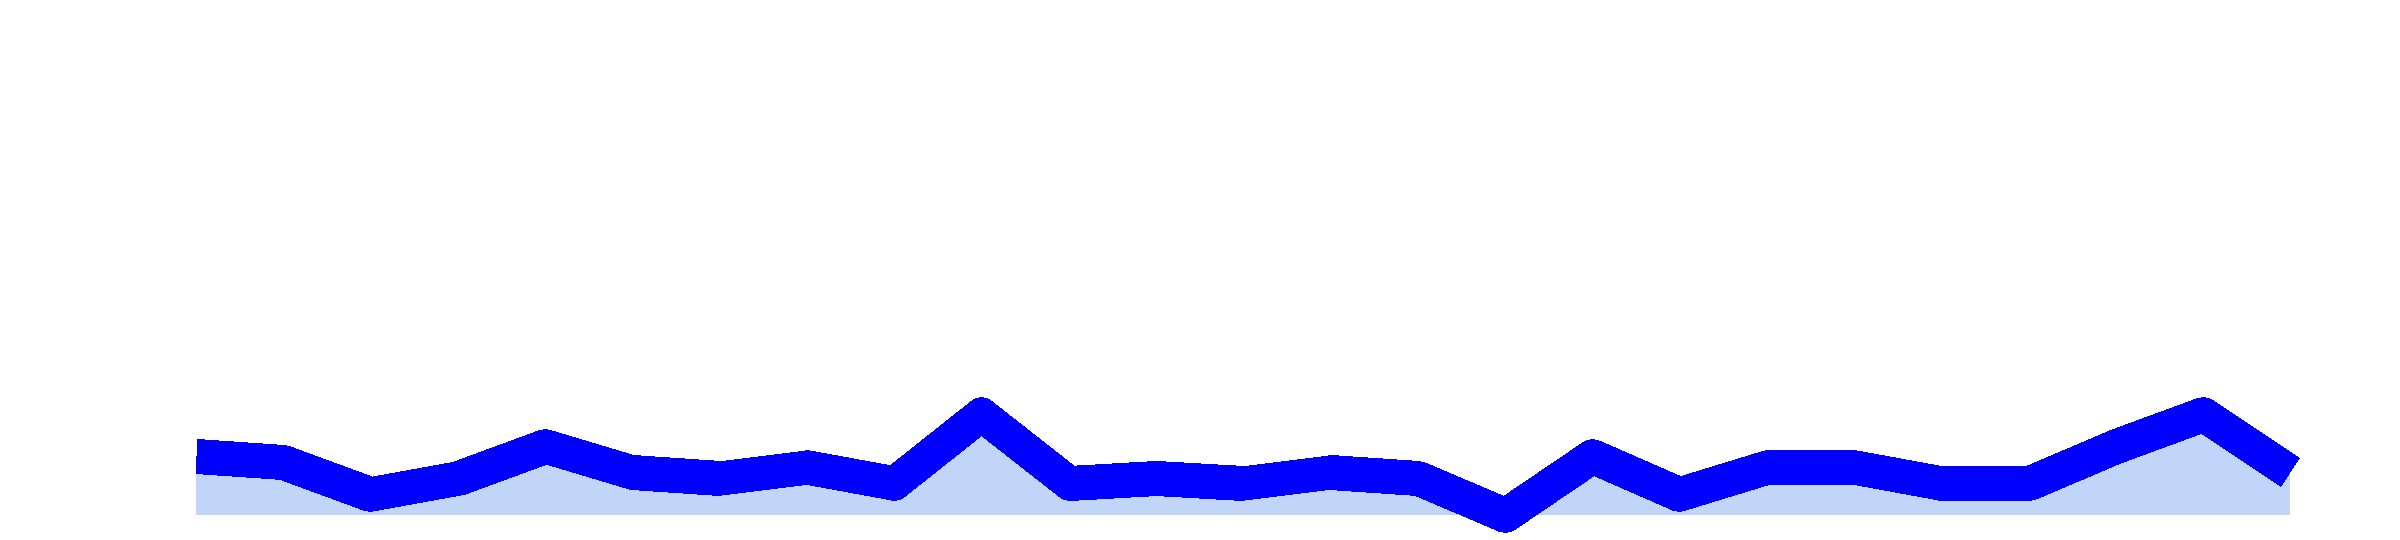
\includegraphics[width=2cm]{fig1.png}} & 1 & 0 & 60 & 61 & 603 & 62 & 62 & 62 & 62 & 62 & 62 & 0.42 & 566 & 639\\
2 & 389 & 195 & \raisebox{.12\height} {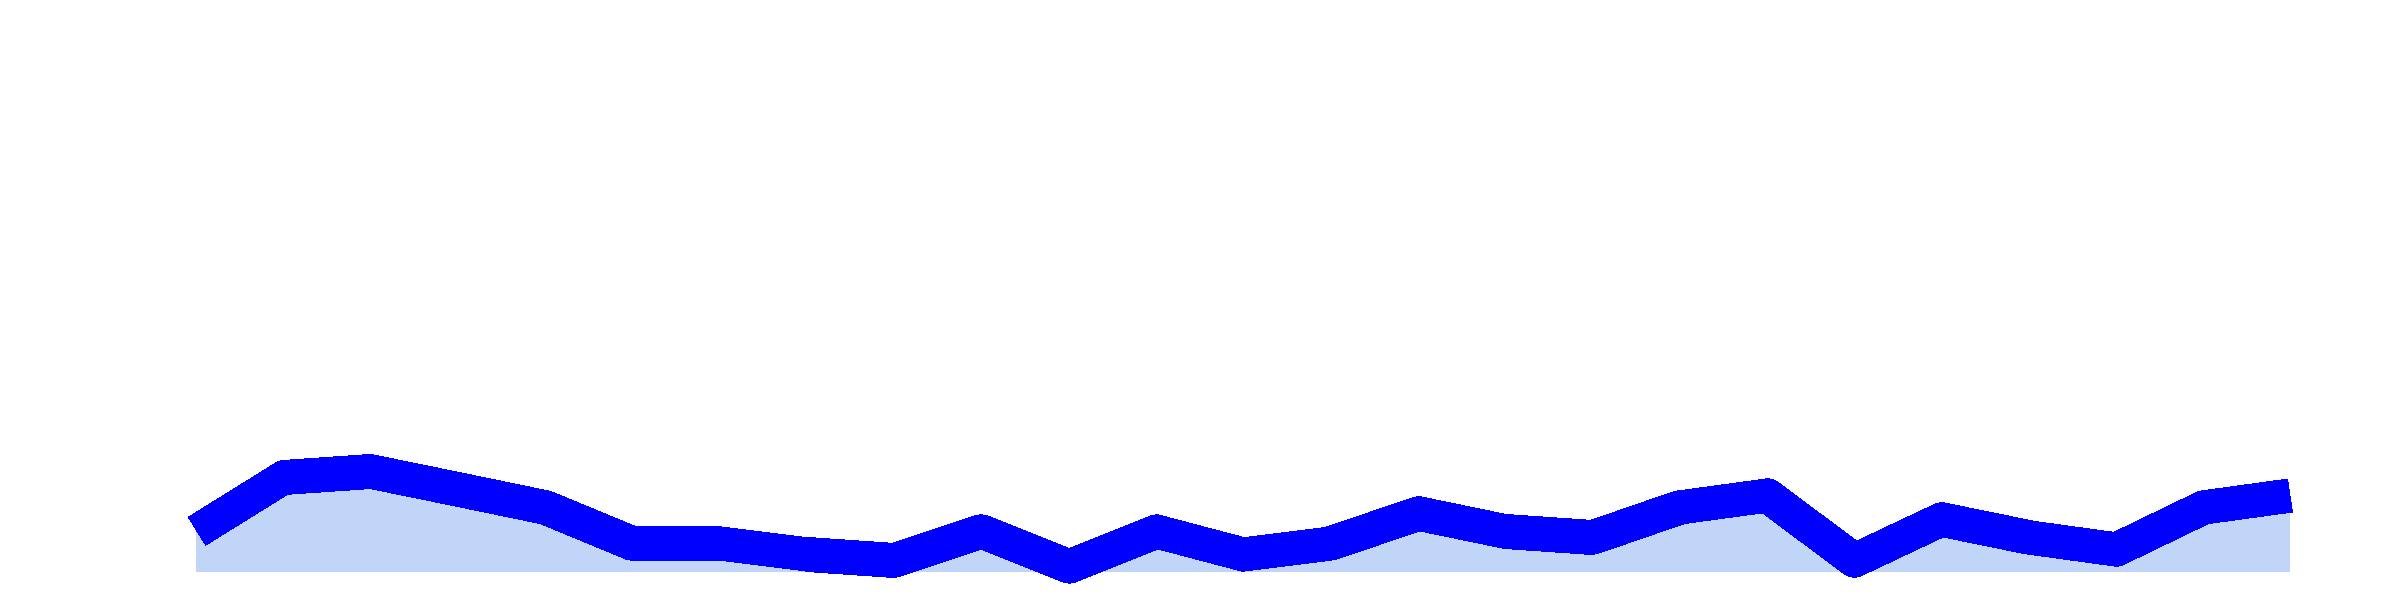
\includegraphics[width=2cm]{fig2.png}} & 1 & 0 & 48 & 49 & 569 & 68 & 68 & 68 & 68 & 68 & 68 & 0.66 & 559 & 603\\
3 & 320 & 167 & \raisebox{.12\height} {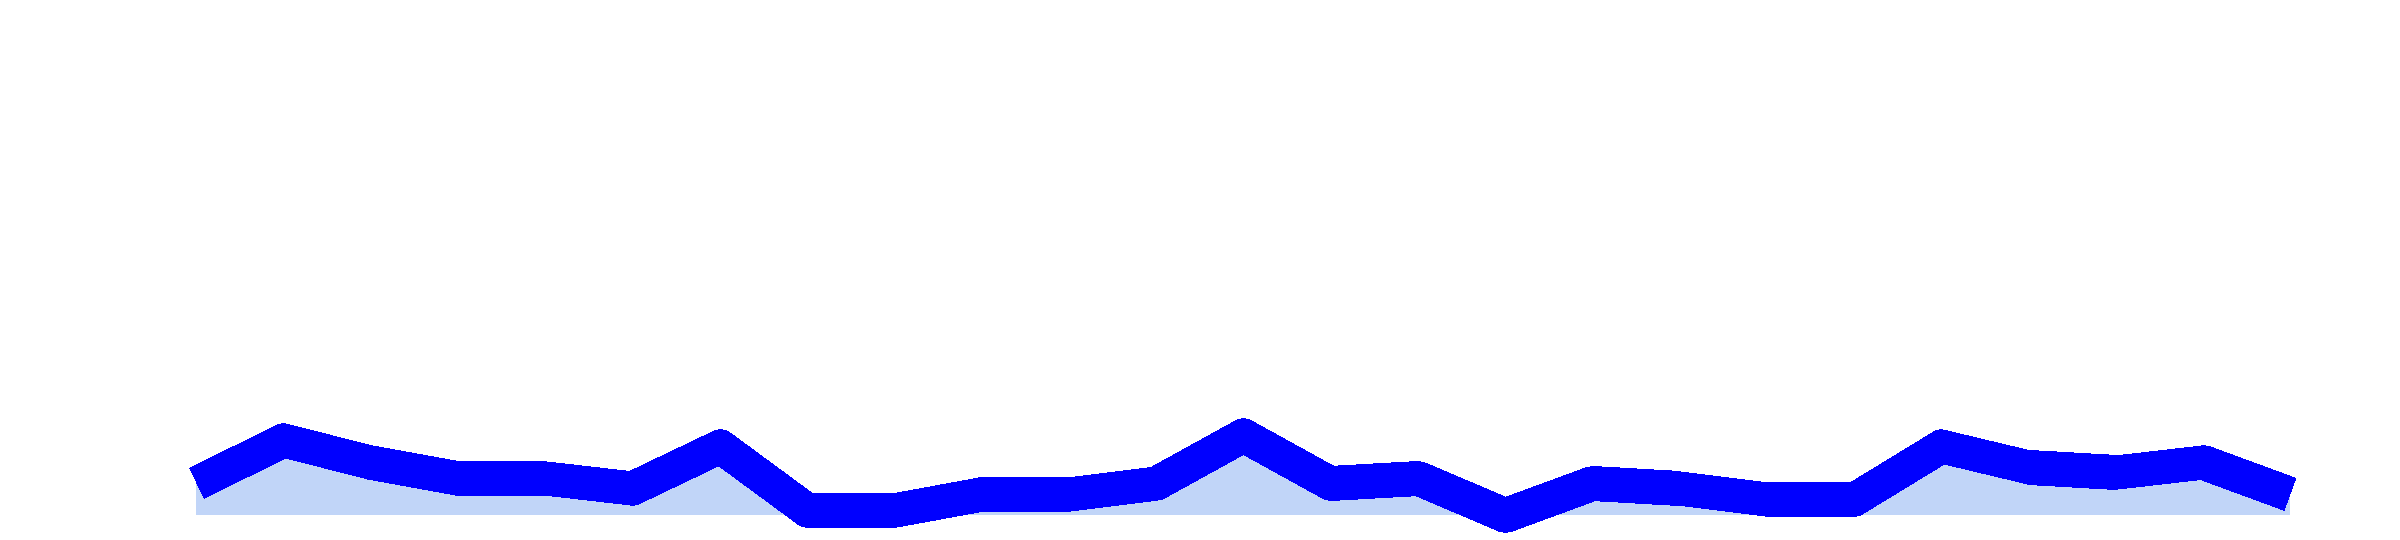
\includegraphics[width=2cm]{fig3.png}} & 0 & 0 & 49 & 49 & 576 & 57 & 57 & 57 & 57 & 57 & 57 & 0.74 & 552 & 615\\
4 & 141 & 45 & \raisebox{.12\height} {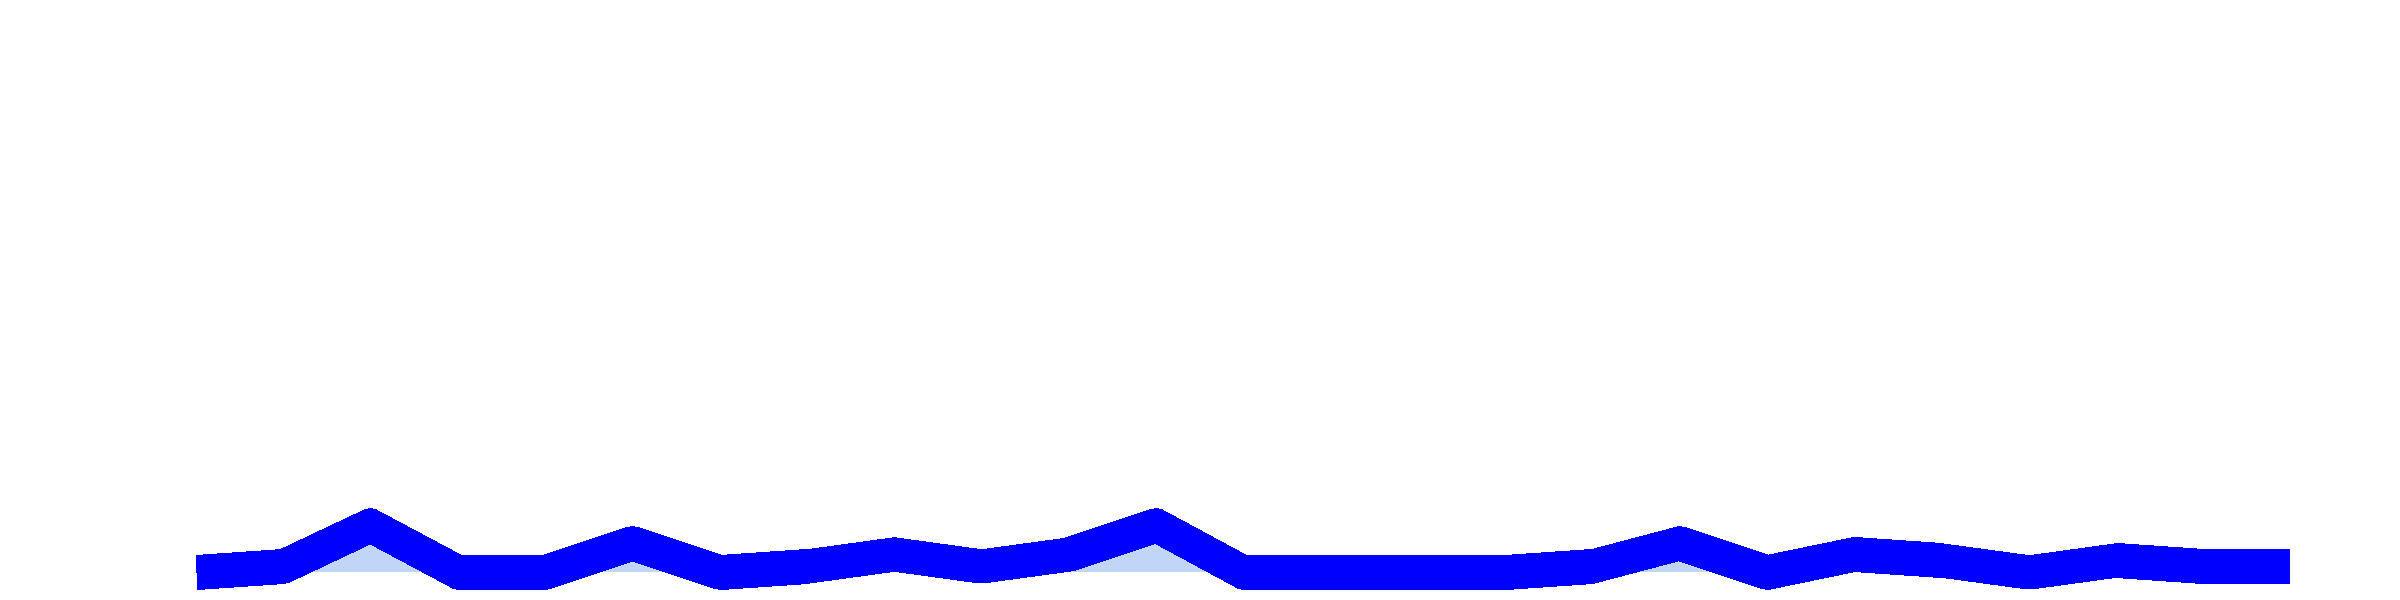
\includegraphics[width=2cm]{fig4.png}} & 0 & 0 & 2 & 2 & 660 & 41 & 41 & 41 & 41 & 41 & 41 & 0.05 & 608 & 650\\
5 & 250 & 69 & \raisebox{.12\height} {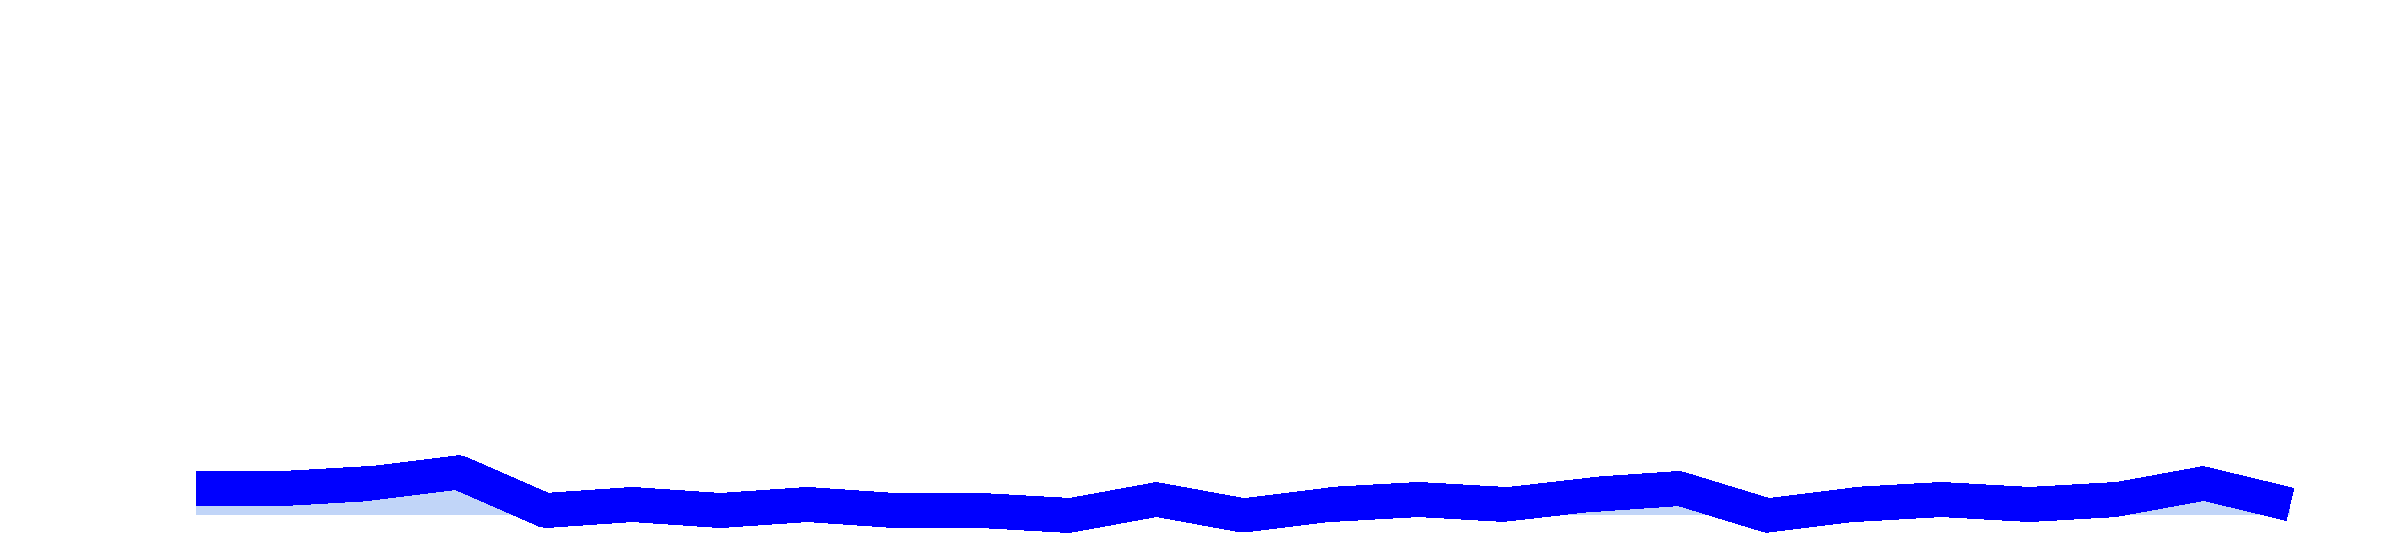
\includegraphics[width=2cm]{fig5.png}} & 1 & 0 & 20 & 21 & 683 & 43 & 43 & 43 & 43 & 43 & 43 & 0.07 & 651 & 676\\
8 & 327 & 169 & \raisebox{.12\height} {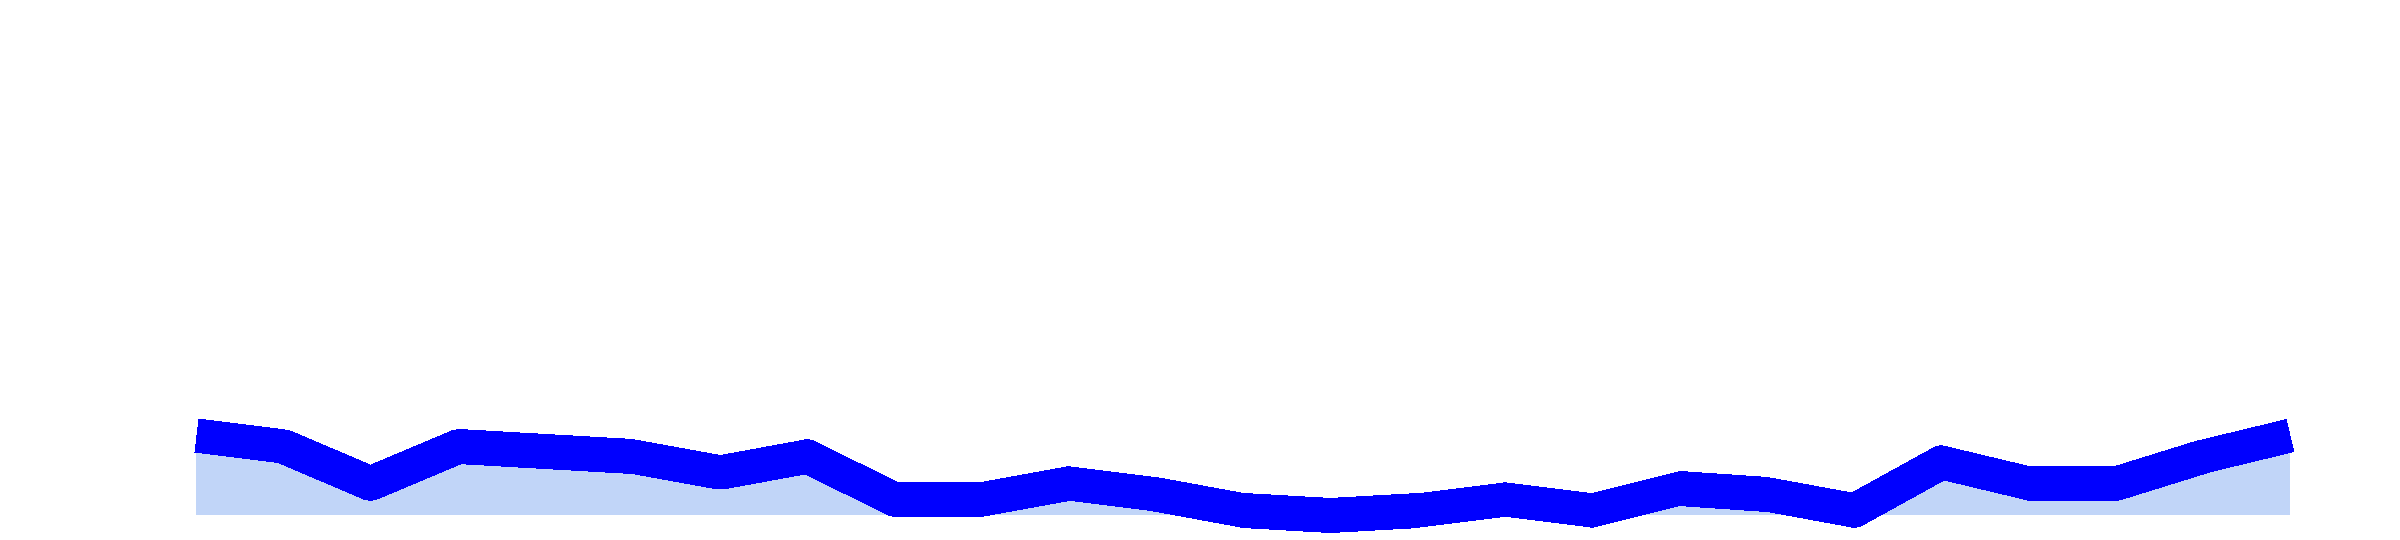
\includegraphics[width=2cm]{fig8.png}} & 0 & 0 & 50 & 50 & 560 & 47 & 47 & 47 & 47 & 47 & 47 & 0.79 & 562 & 601\\
9 & 603 & 275 & \raisebox{.12\height} {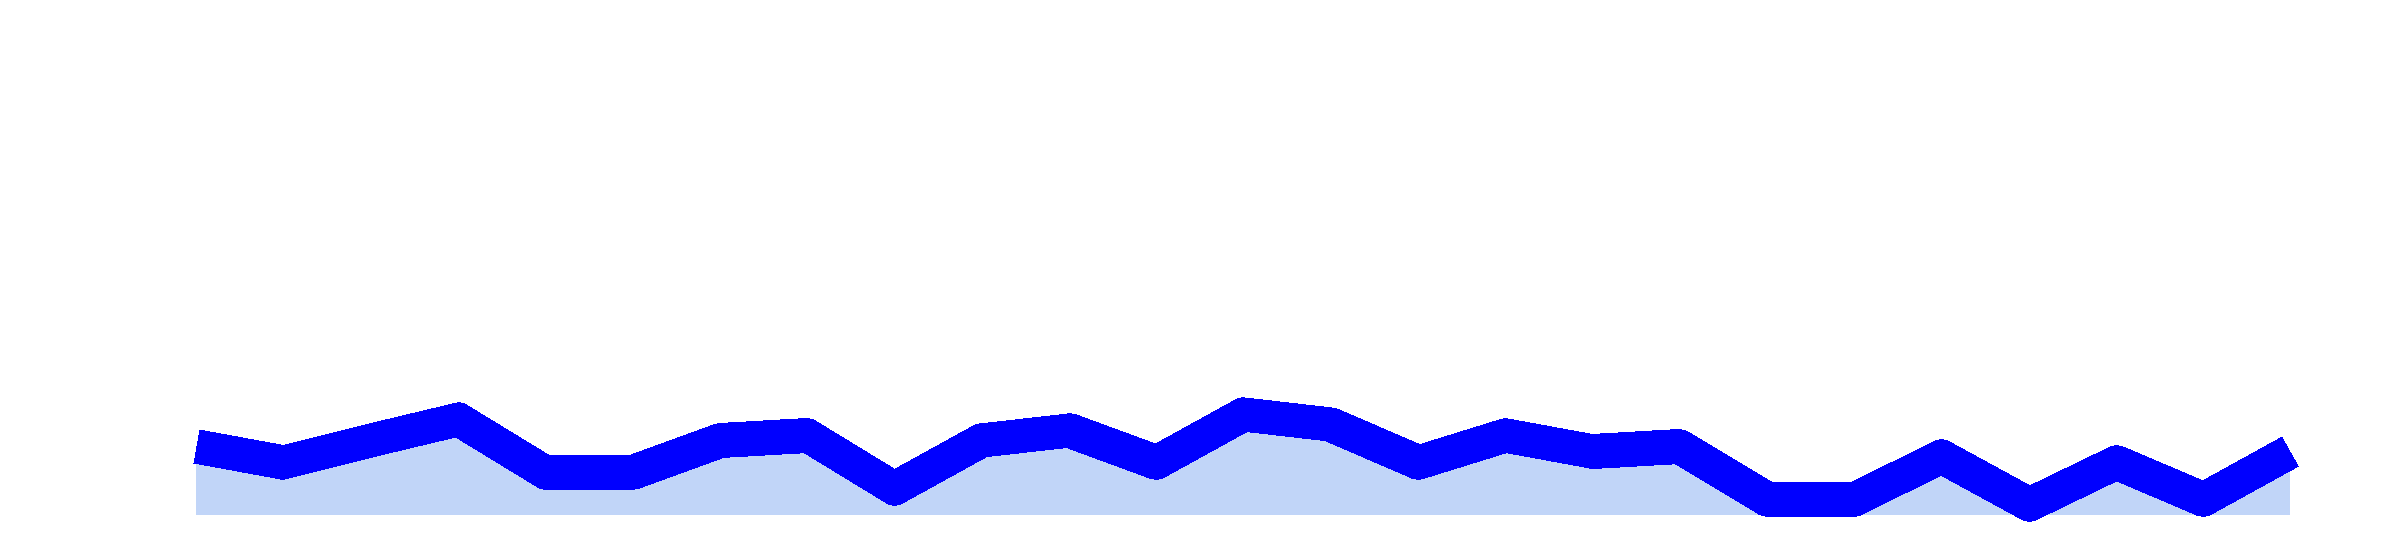
\includegraphics[width=2cm]{fig9.png}} & 0 & 0 & 74 & 74 & 597 & 47 & 47 & 47 & 47 & 47 & 47 & 0.53 & 576 & 623\\
10 & 336 & 164 & \raisebox{.12\height} {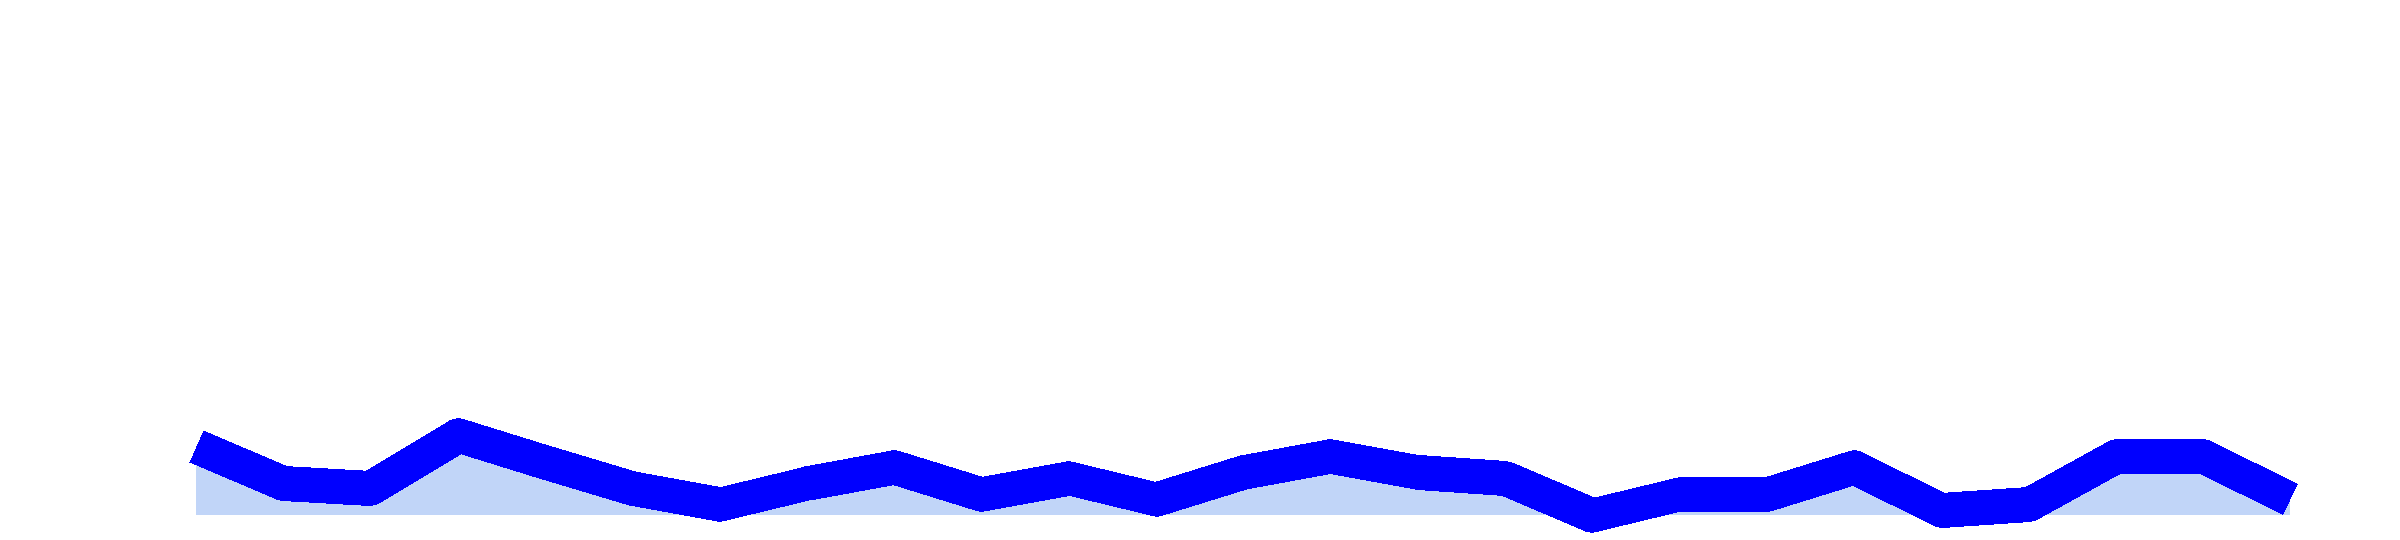
\includegraphics[width=2cm]{fig10.png}} & 0 & 0 & 58 & 58 & 568 & 55 & 55 & 55 & 55 & 55 & 55 & 0.80 & 553 & 624\\
11 & 192 & 66 & \raisebox{.12\height} {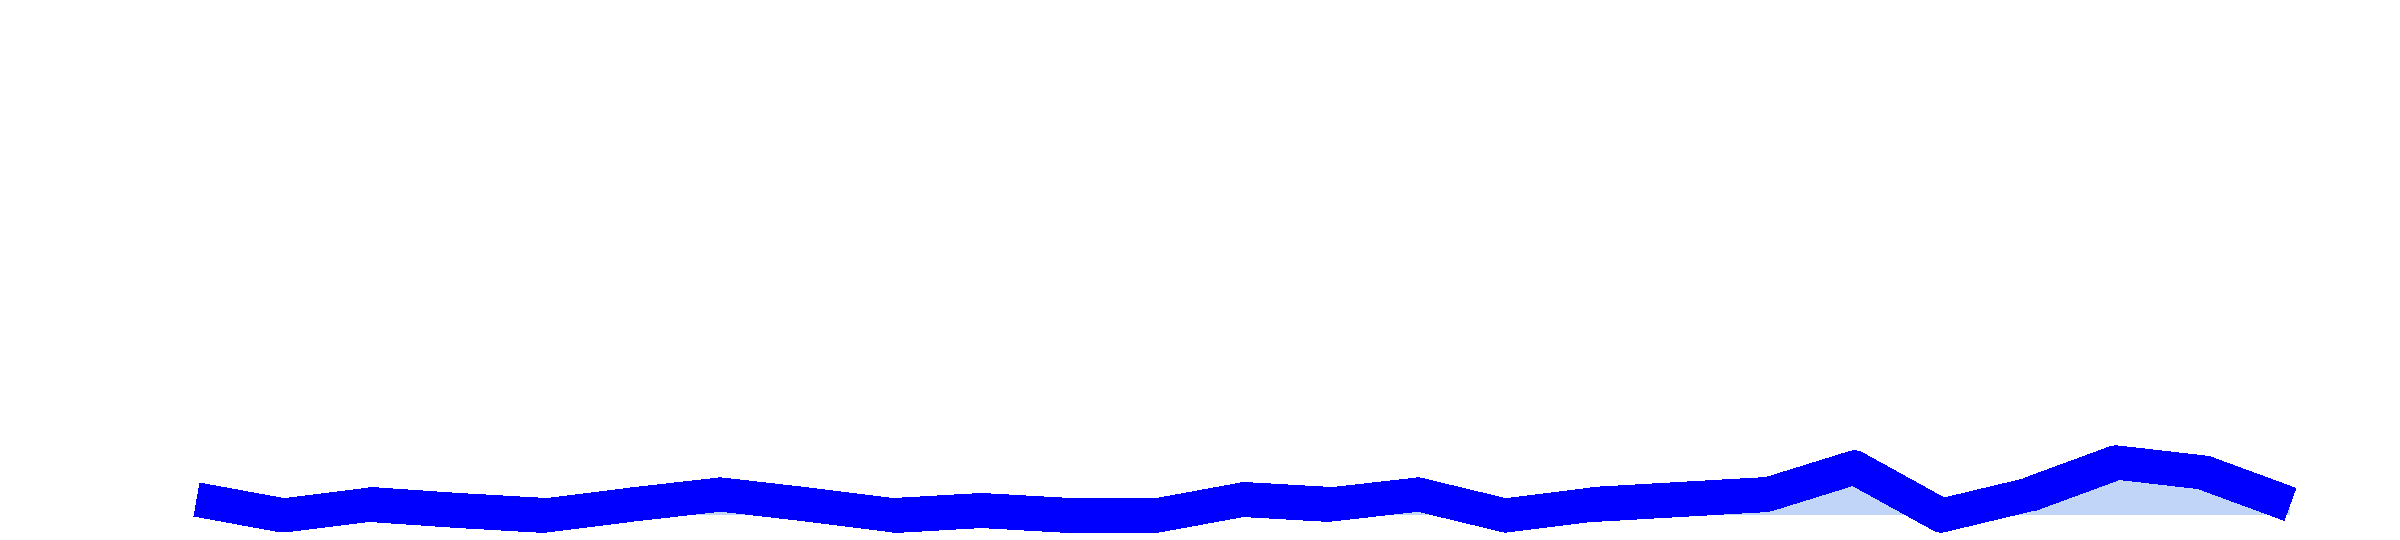
\includegraphics[width=2cm]{fig11.png}} & 0 & 0 & 19 & 19 & 623 & 44 & 44 & 44 & 44 & 44 & 44 & 0.25 & 588 & 643\\
12 & 206 & 89 & \raisebox{.12\height} {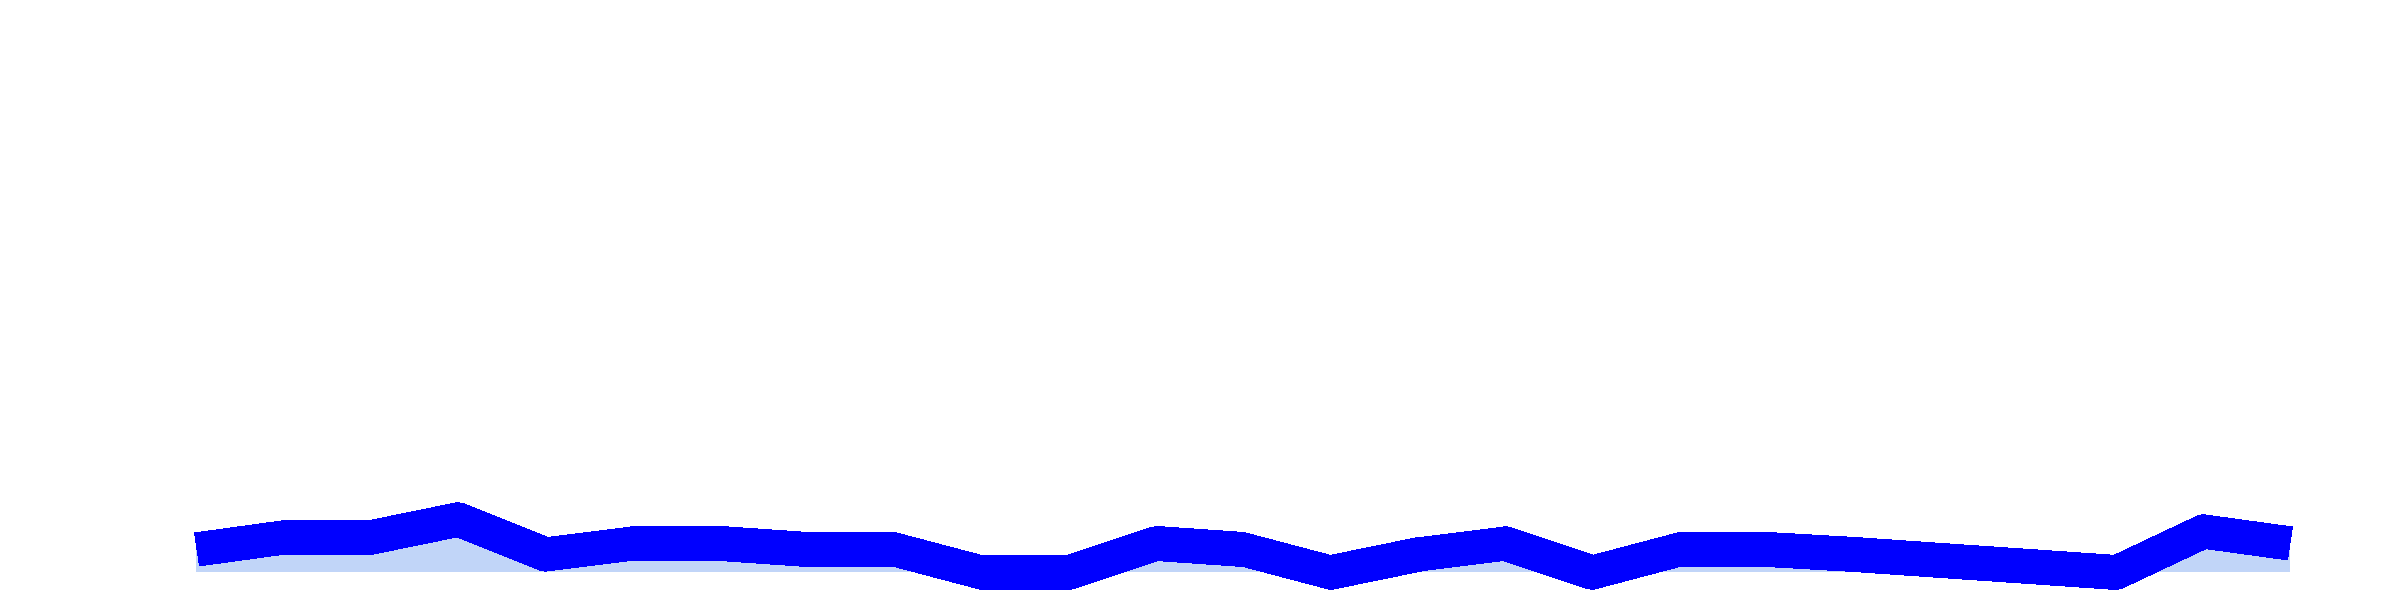
\includegraphics[width=2cm]{fig12.png}} & 0 & 0 & 37 & 37 & 611 & 39 & 39 & 39 & 39 & 39 & 39 & 0.69 & 588 & 593\\
13 & 730 & 432 & \raisebox{.12\height} {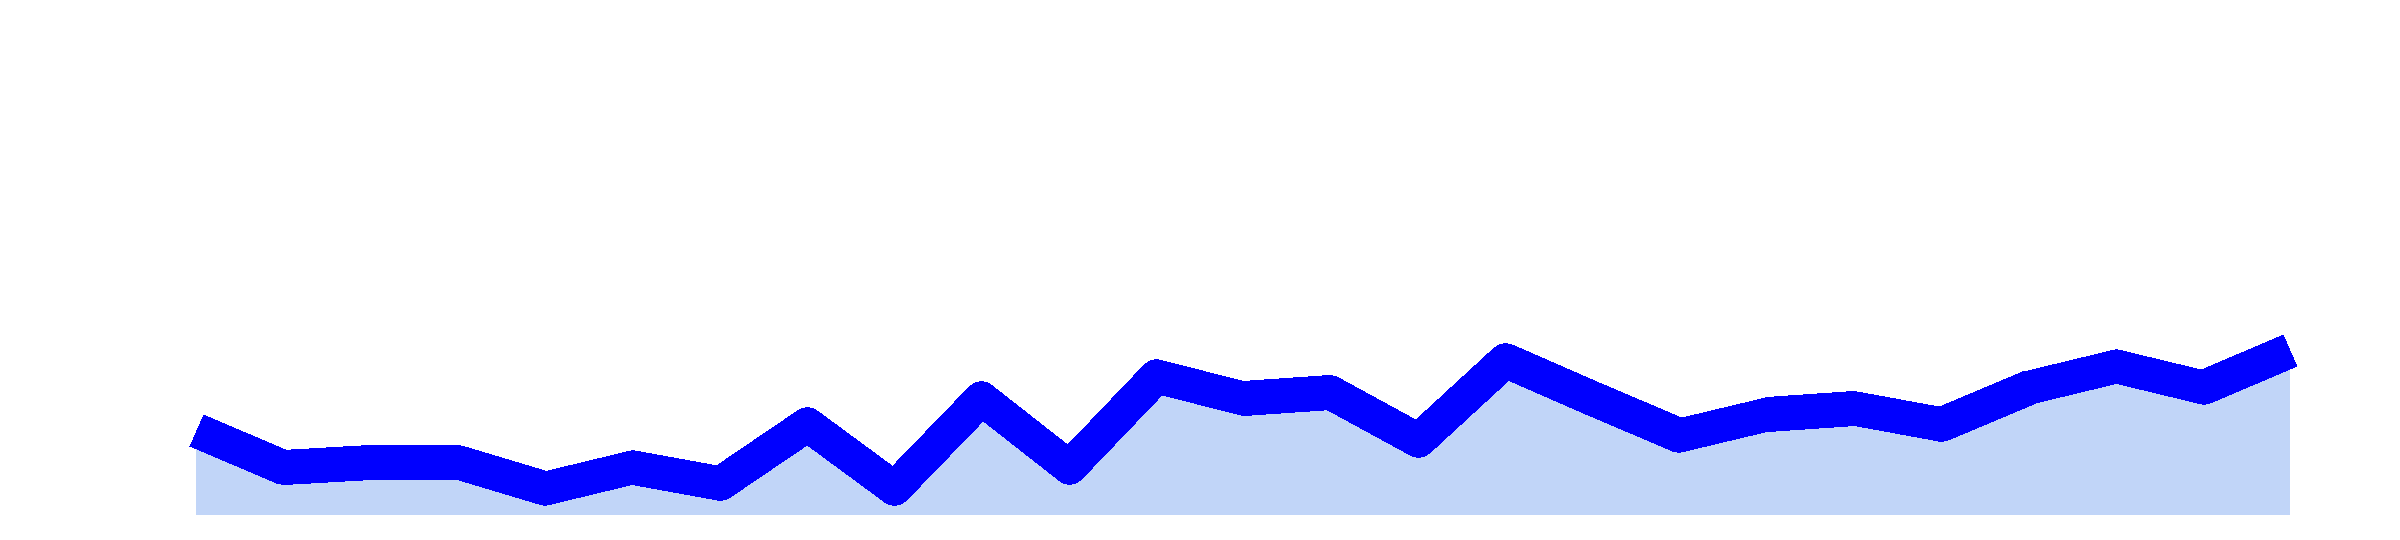
\includegraphics[width=2cm]{fig13.png}} & 1 & 0 & 131 & 132 & 525 & 44 & 44 & 44 & 44 & 44 & 44 & 0.80 & 525 & 539\\
14 & 206 & 83 & \raisebox{.12\height} {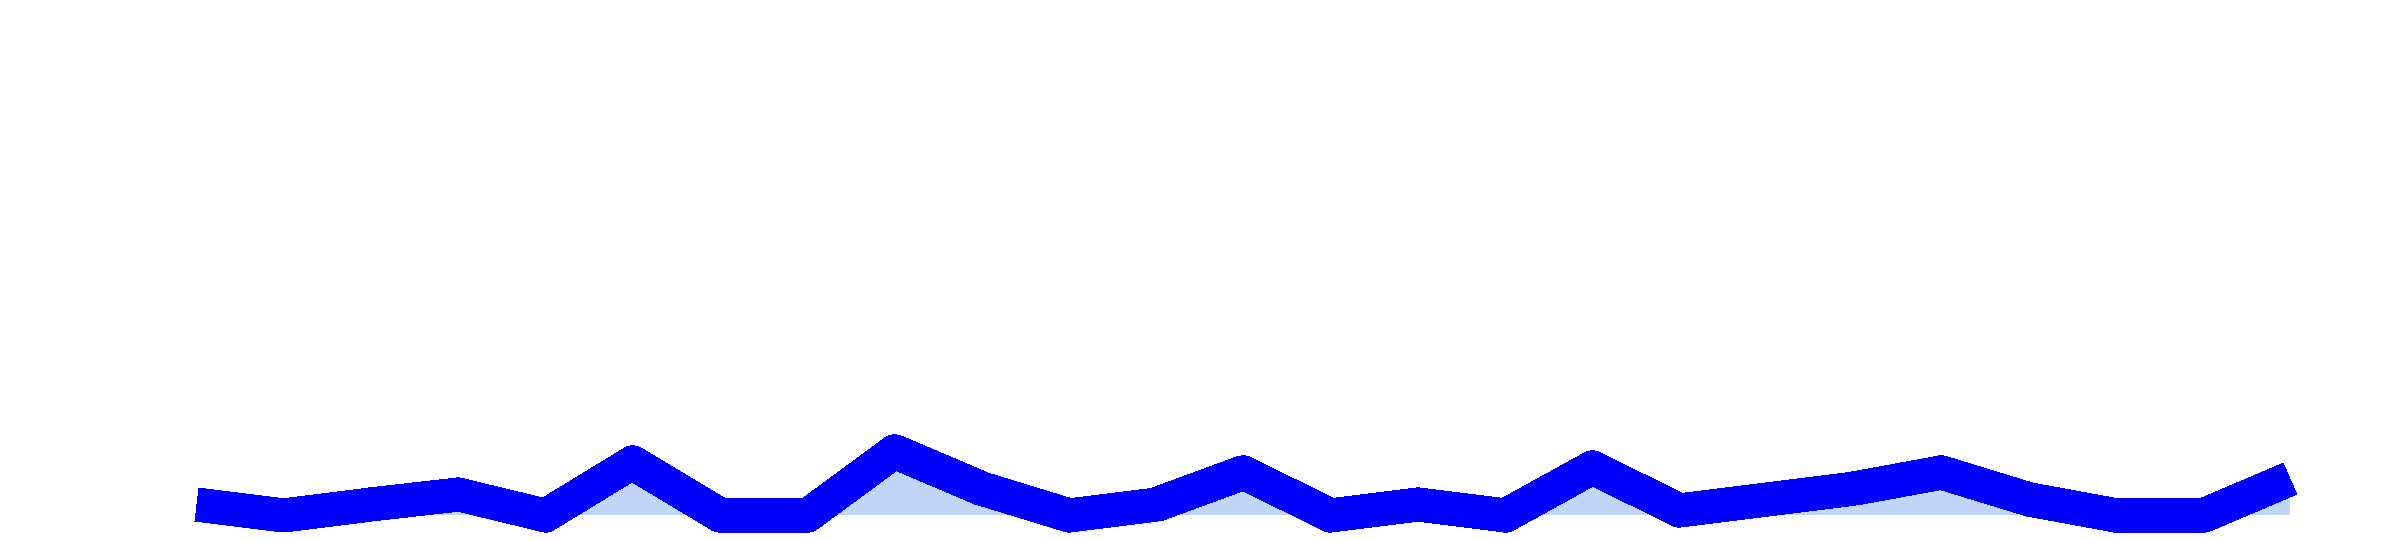
\includegraphics[width=2cm]{fig14.png}} & 0 & 0 & 32 & 32 & 601 & 41 & 41 & 41 & 41 & 41 & 41 & 0.63 & 600 & 598\\
15 & 893 & 315 & \raisebox{.12\height} {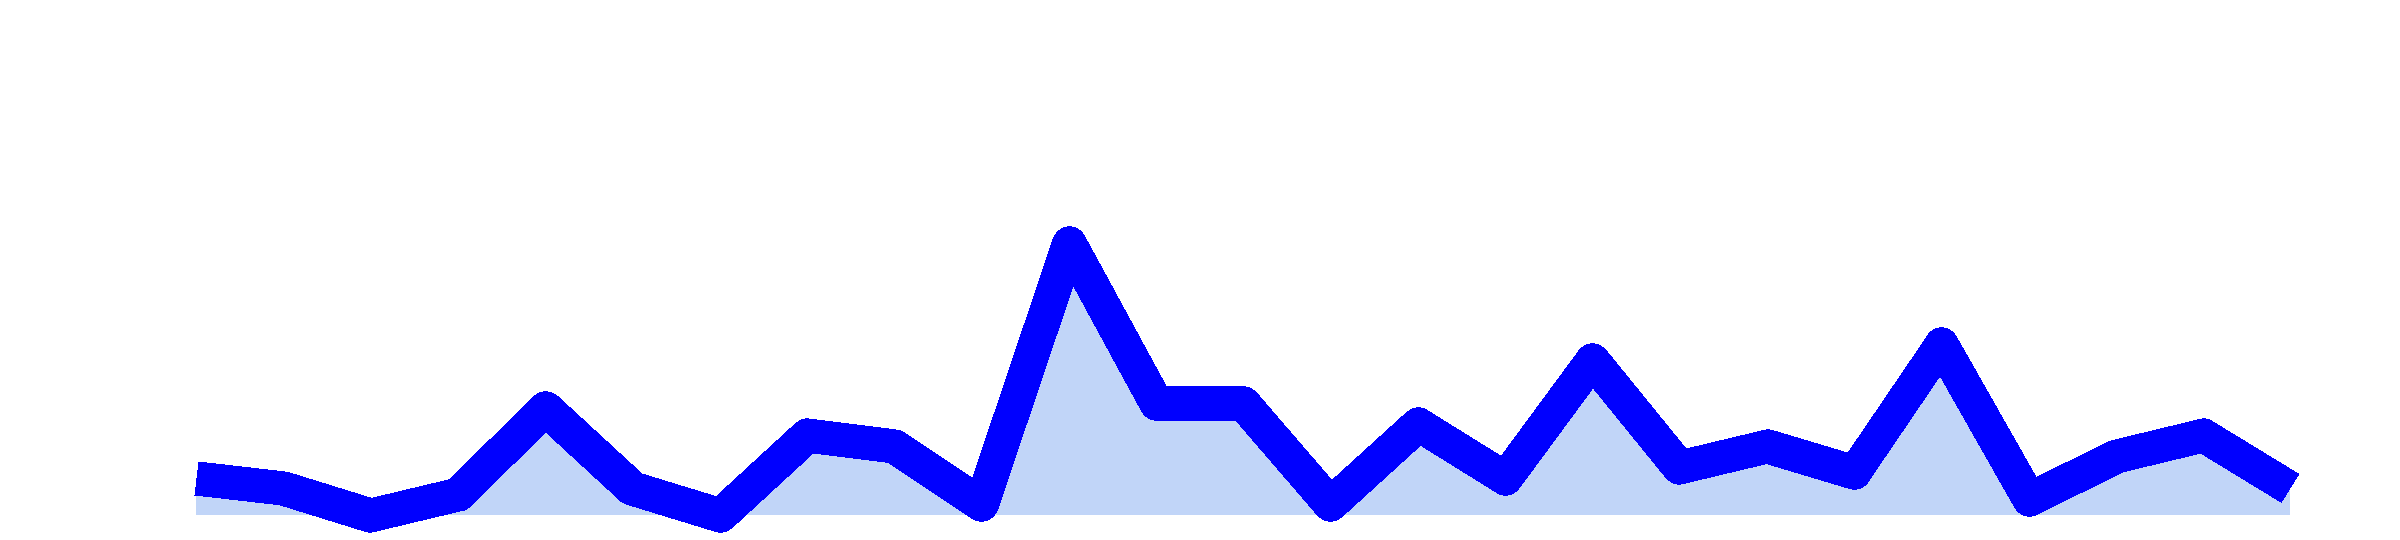
\includegraphics[width=2cm]{fig15.png}} & 2 & 0 & 61 & 63 & 629 & 84 & 84 & 84 & 84 & 84 & 84 & 0.36 & 618 & 639\\
16 & 277 & 97 & \raisebox{.12\height} {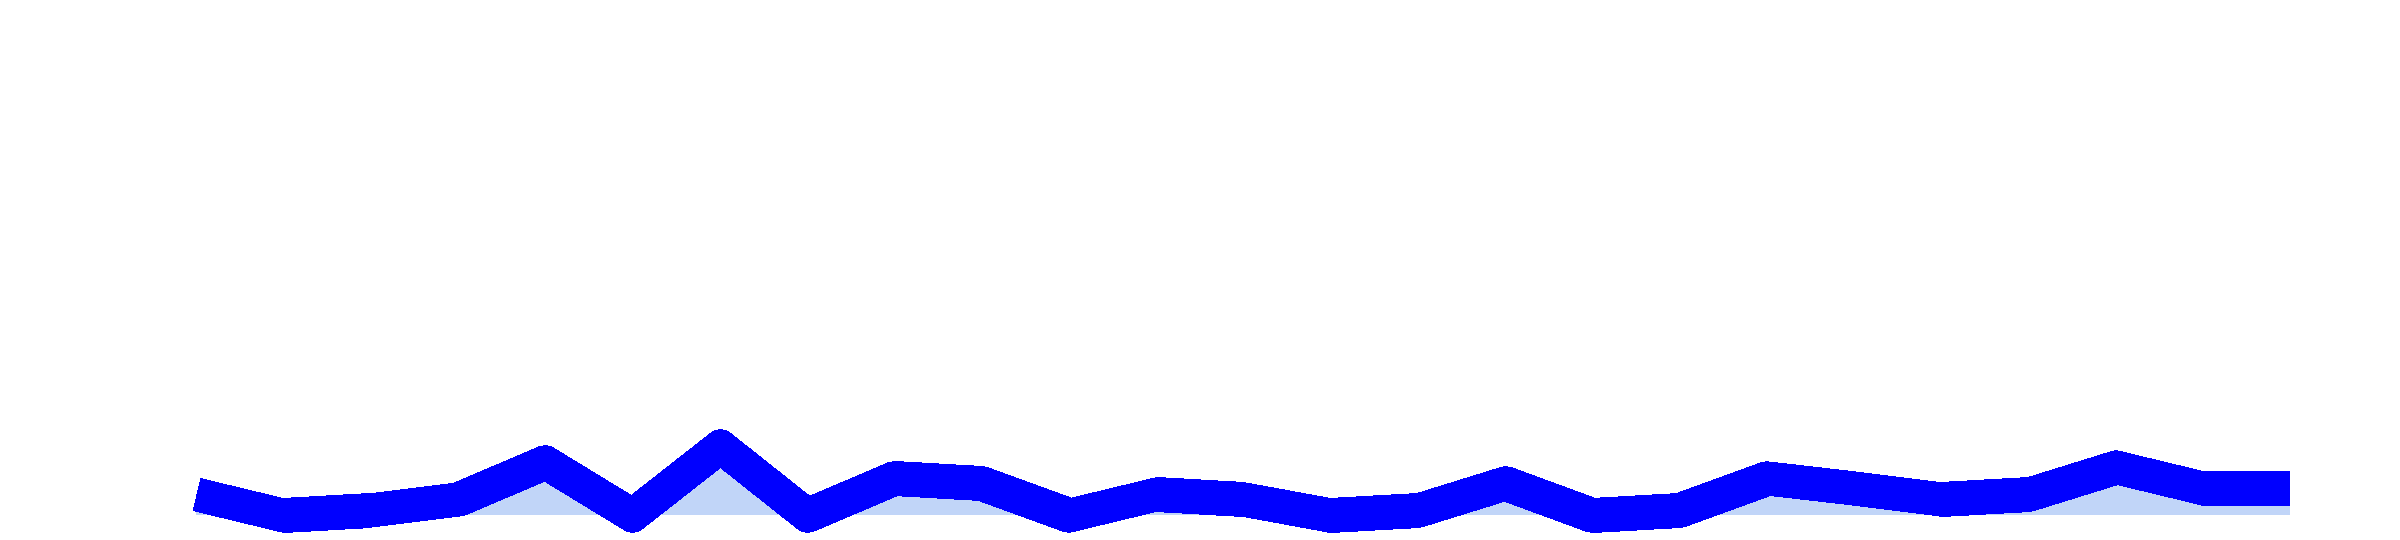
\includegraphics[width=2cm]{fig16.png}} & 0 & 0 & 31 & 31 & 607 & 48 & 48 & 48 & 48 & 48 & 48 & 0.48 & 616 & 659\\
17 & 208 & 44 & \raisebox{.12\height} {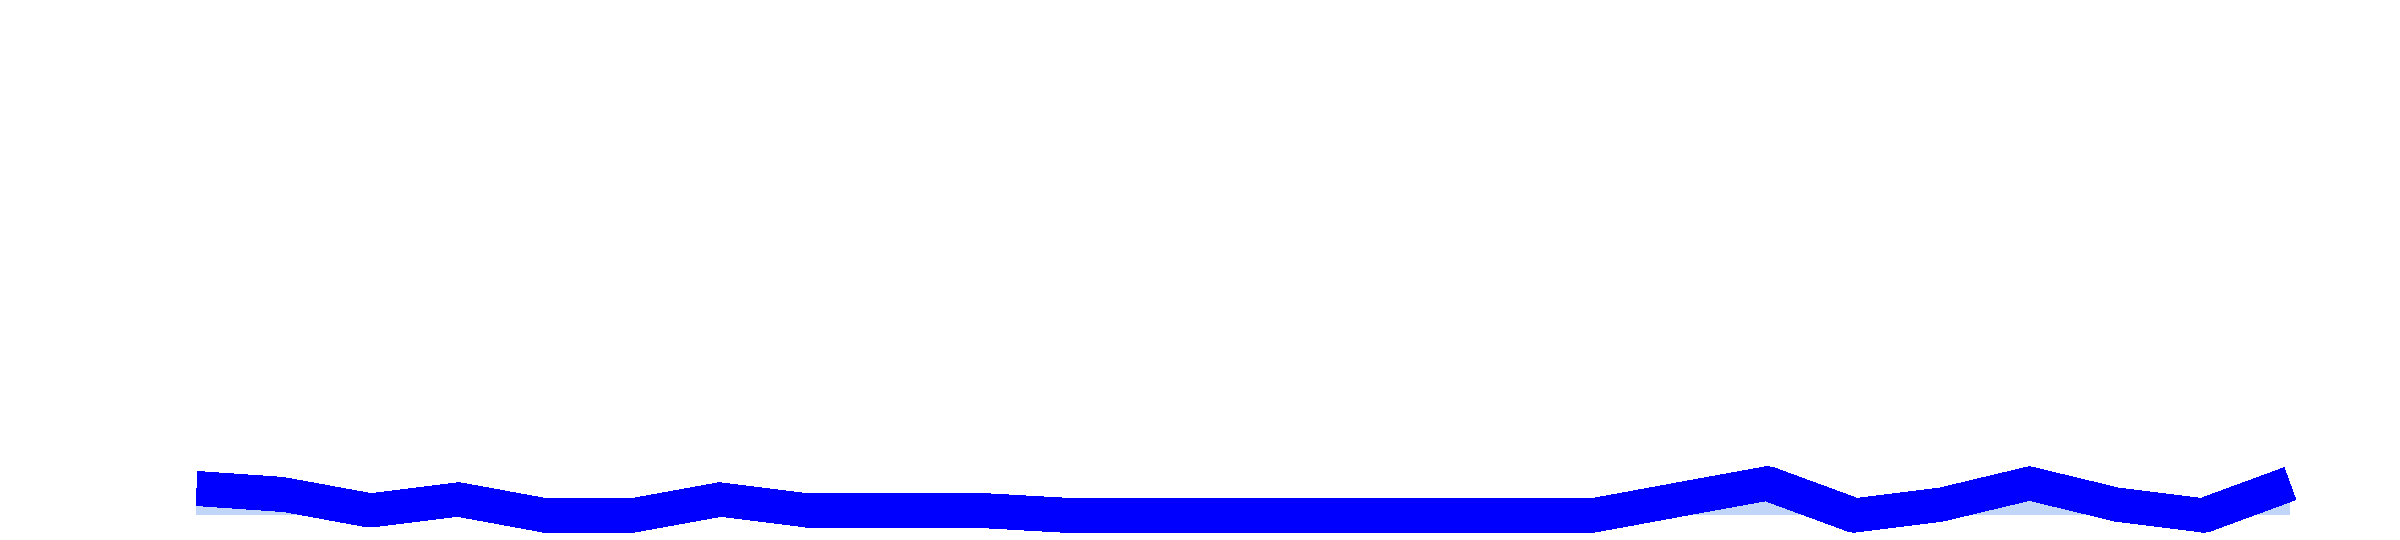
\includegraphics[width=2cm]{fig17.png}} & 0 & 0 & 27 & 27 & 719 & 10 & 10 & 10 & 10 & 10 & 10 & 0.10 & 618 & 761\\
18 & 263 & 76 & \raisebox{.12\height} {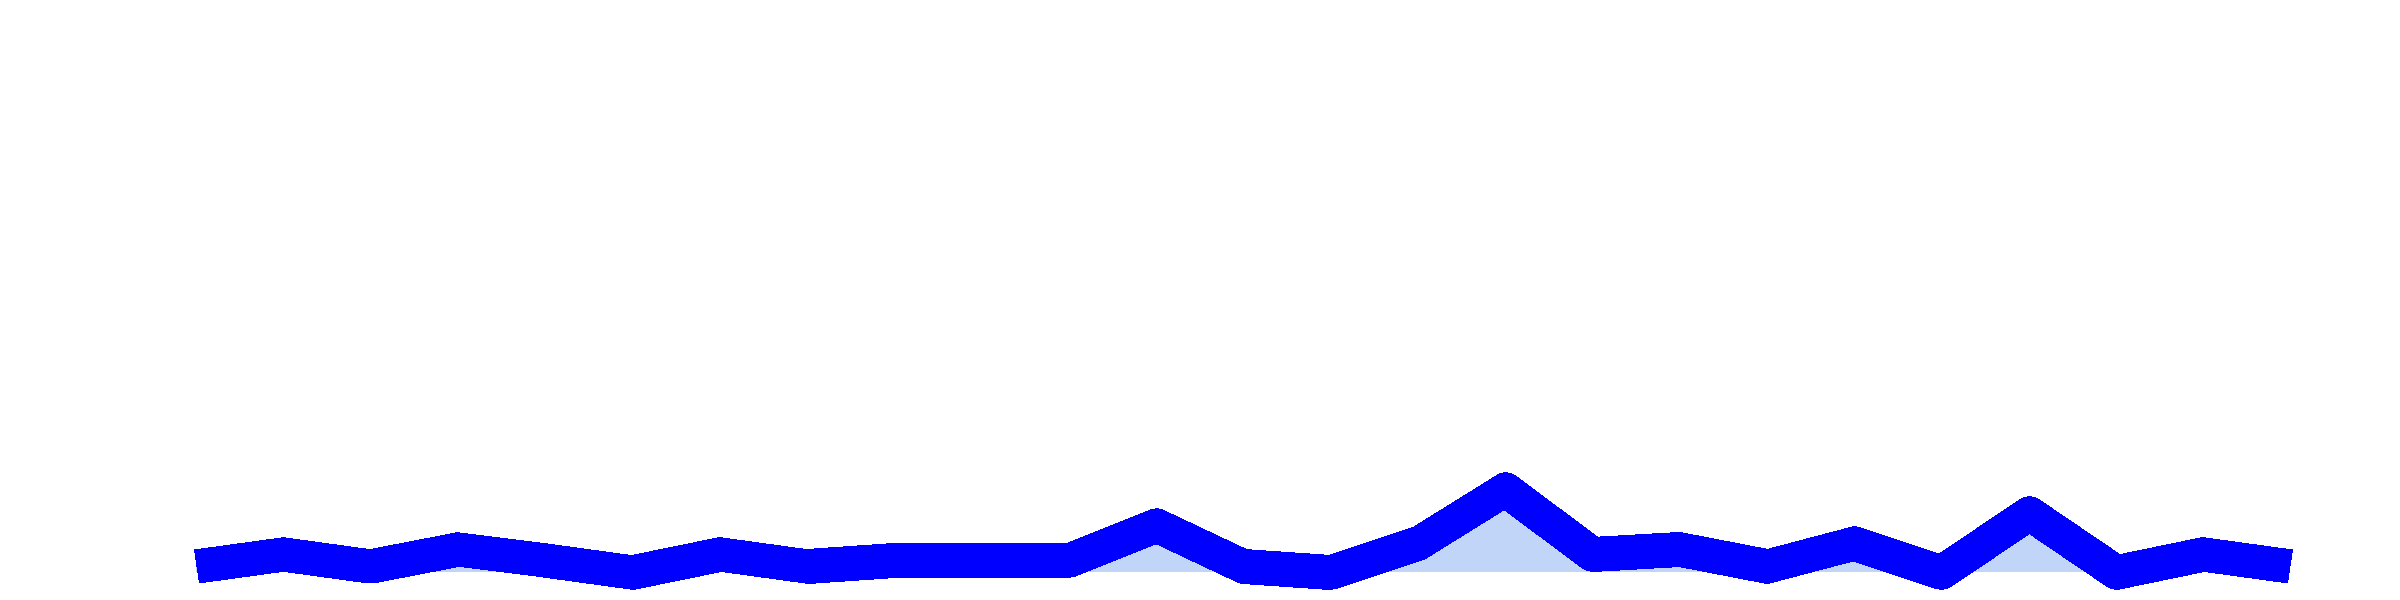
\includegraphics[width=2cm]{fig18.png}} & 0 & 0 & 16 & 16 & 660 & 52 & 52 & 52 & 52 & 52 & 52 & 0.06 & 648 & 673\\
19 & 369 & 194 & \raisebox{.12\height} {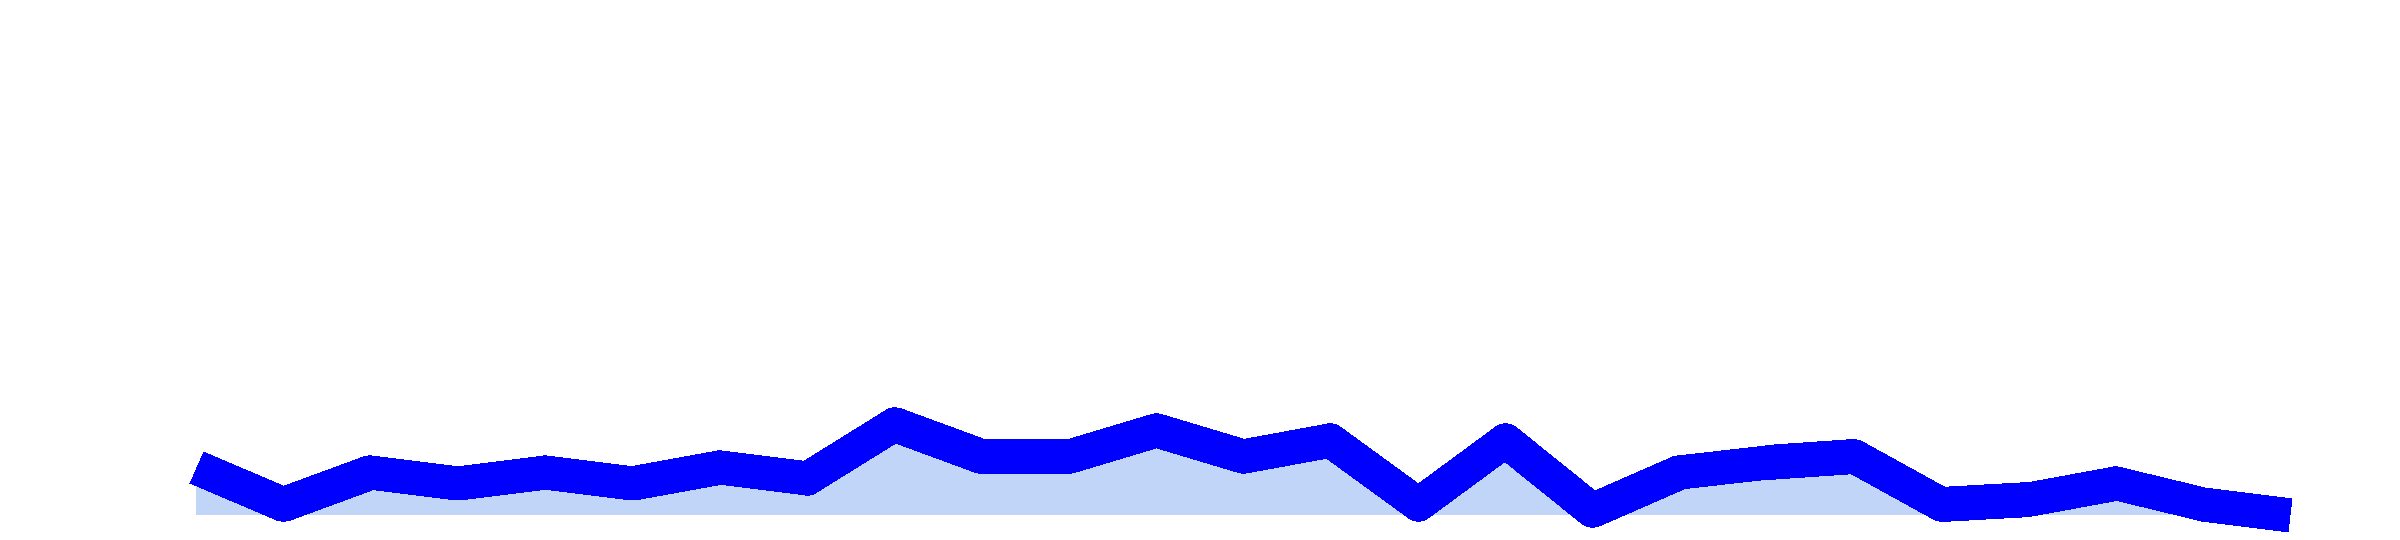
\includegraphics[width=2cm]{fig19.png}} & 1 & 0 & 60 & 61 & 567 & 49 & 49 & 49 & 49 & 49 & 49 & 0.82 & 532 & 630\\
20 & 710 & 451 & \raisebox{.12\height} {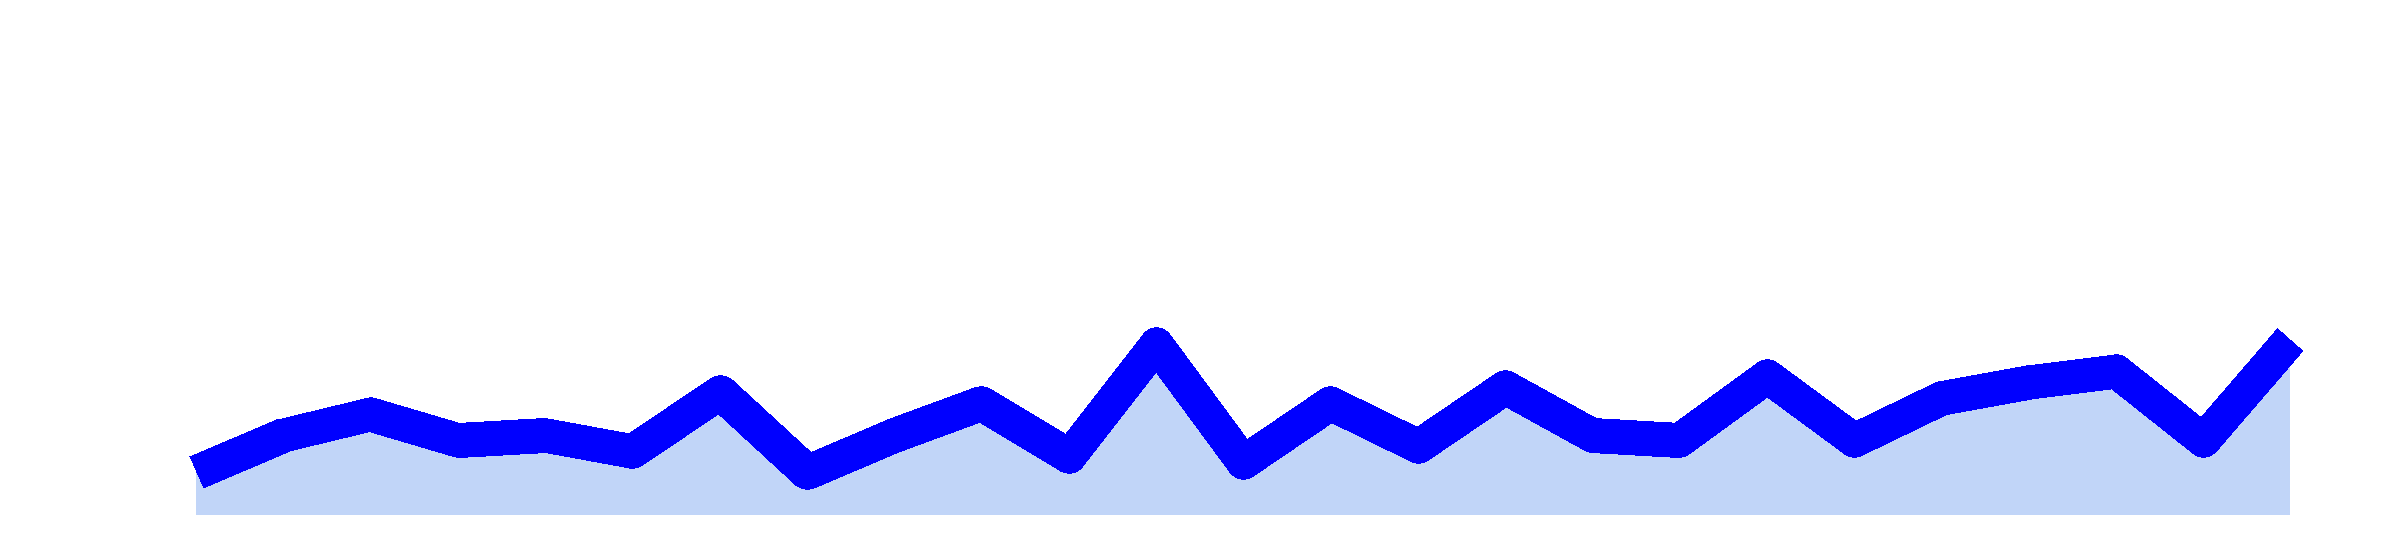
\includegraphics[width=2cm]{fig20.png}} & 2 & 0 & 184 & 186 & 519 & 56 & 56 & 56 & 56 & 56 & 56 & 0.82 & 525 & 514\\
21 & 444 & 178 & \raisebox{.12\height} {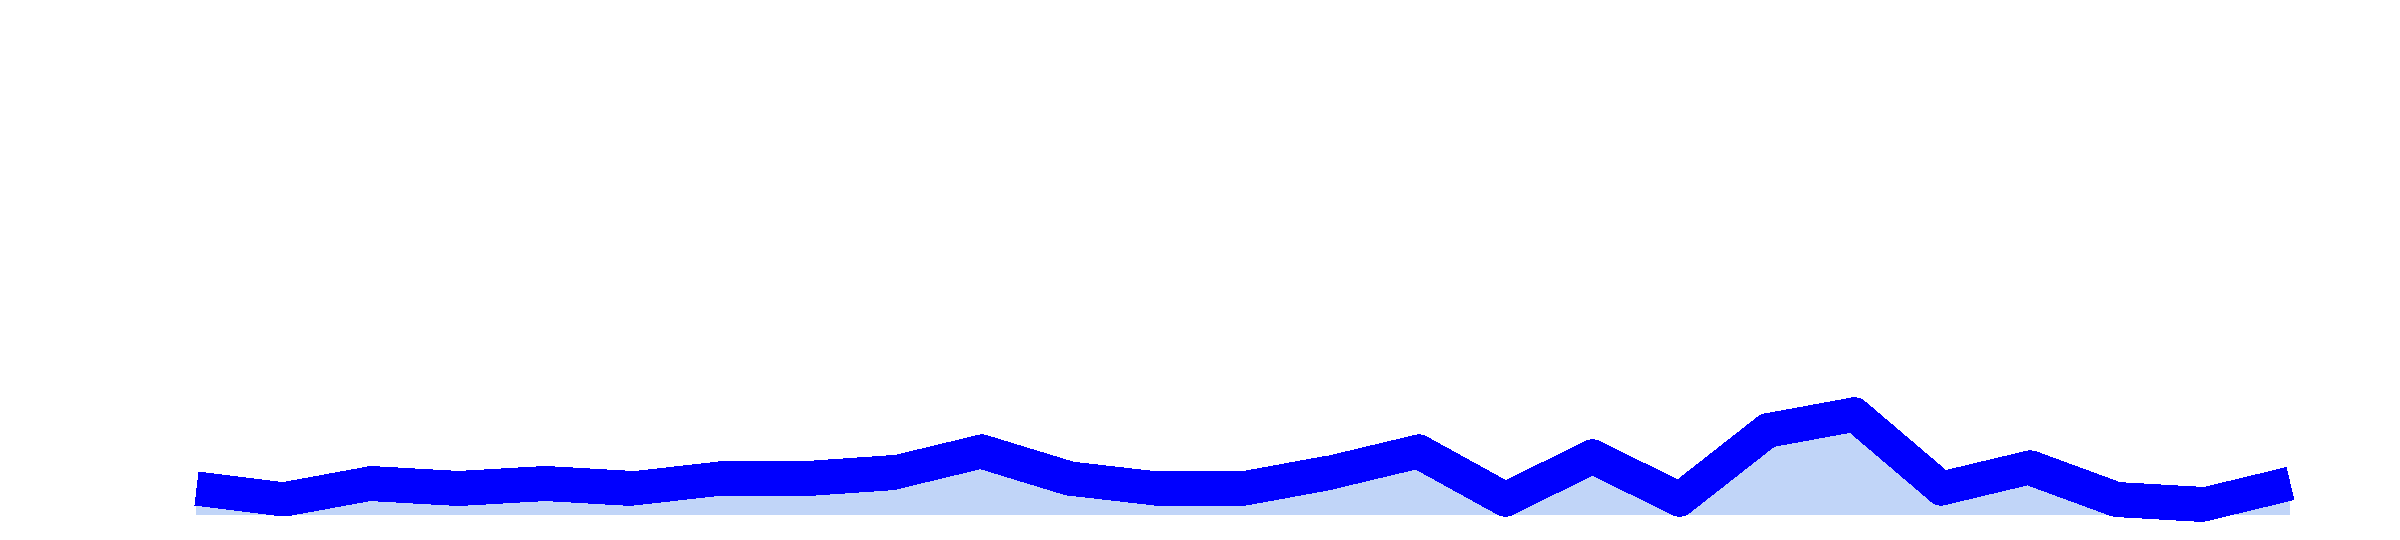
\includegraphics[width=2cm]{fig21.png}} & 0 & 0 & 45 & 45 & 605 & 62 & 62 & 62 & 62 & 62 & 62 & 0.66 & 588 & 679\\
22 & 418 & 226 & \raisebox{.12\height} {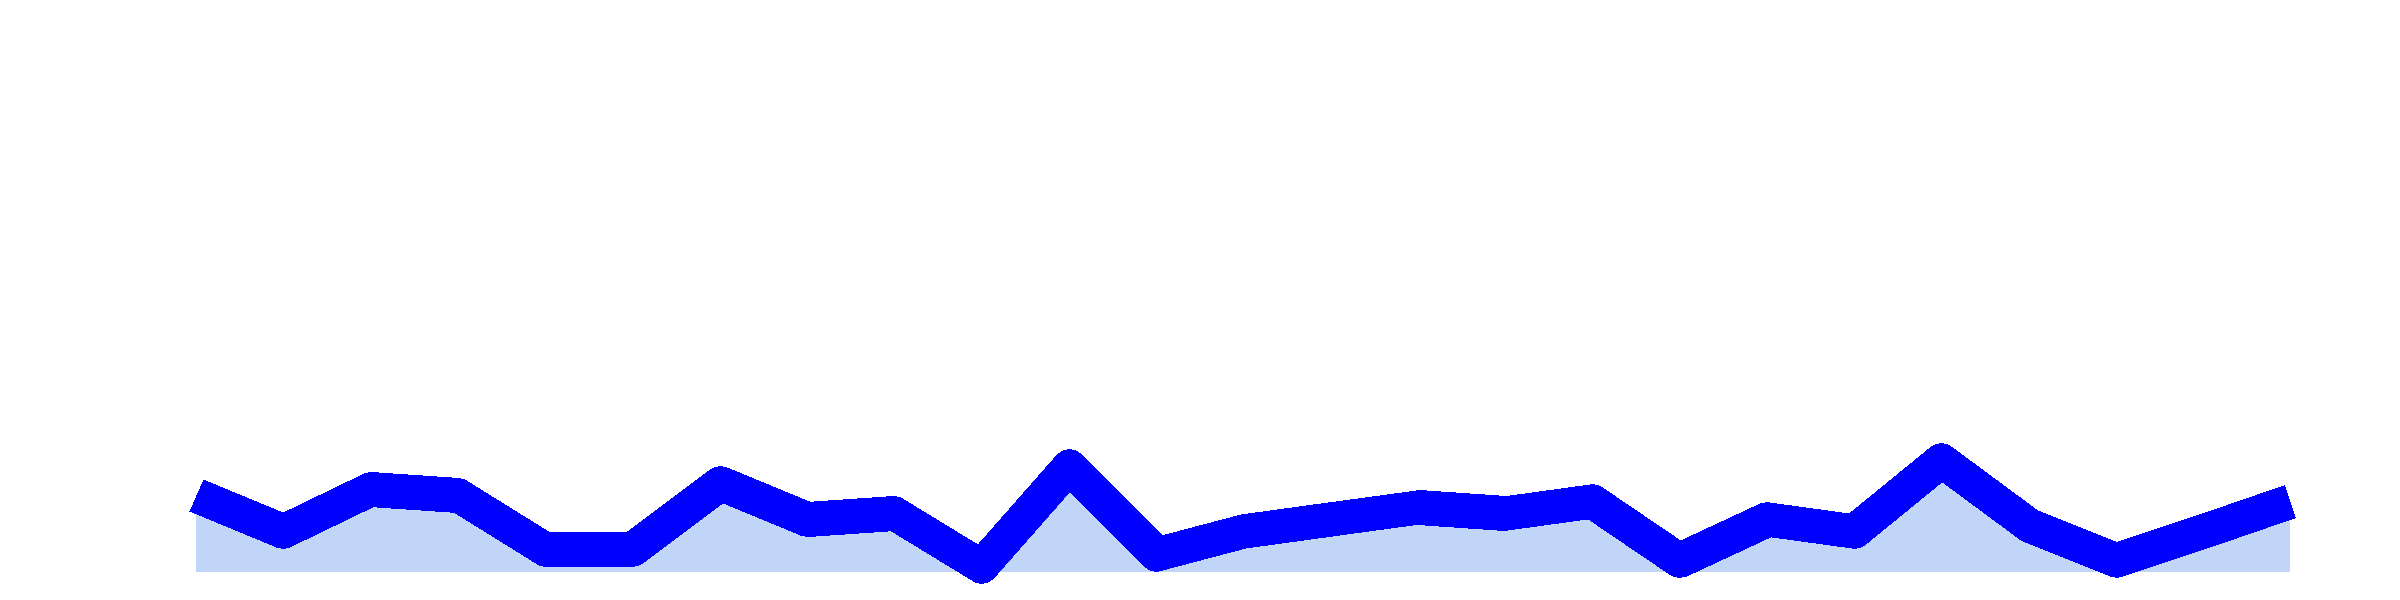
\includegraphics[width=2cm]{fig22.png}} & 2 & 0 & 87 & 89 & 568 & 63 & 63 & 63 & 63 & 63 & 63 & 0.65 & 542 & 556\\
23 & 265 & 154 & \raisebox{.12\height} {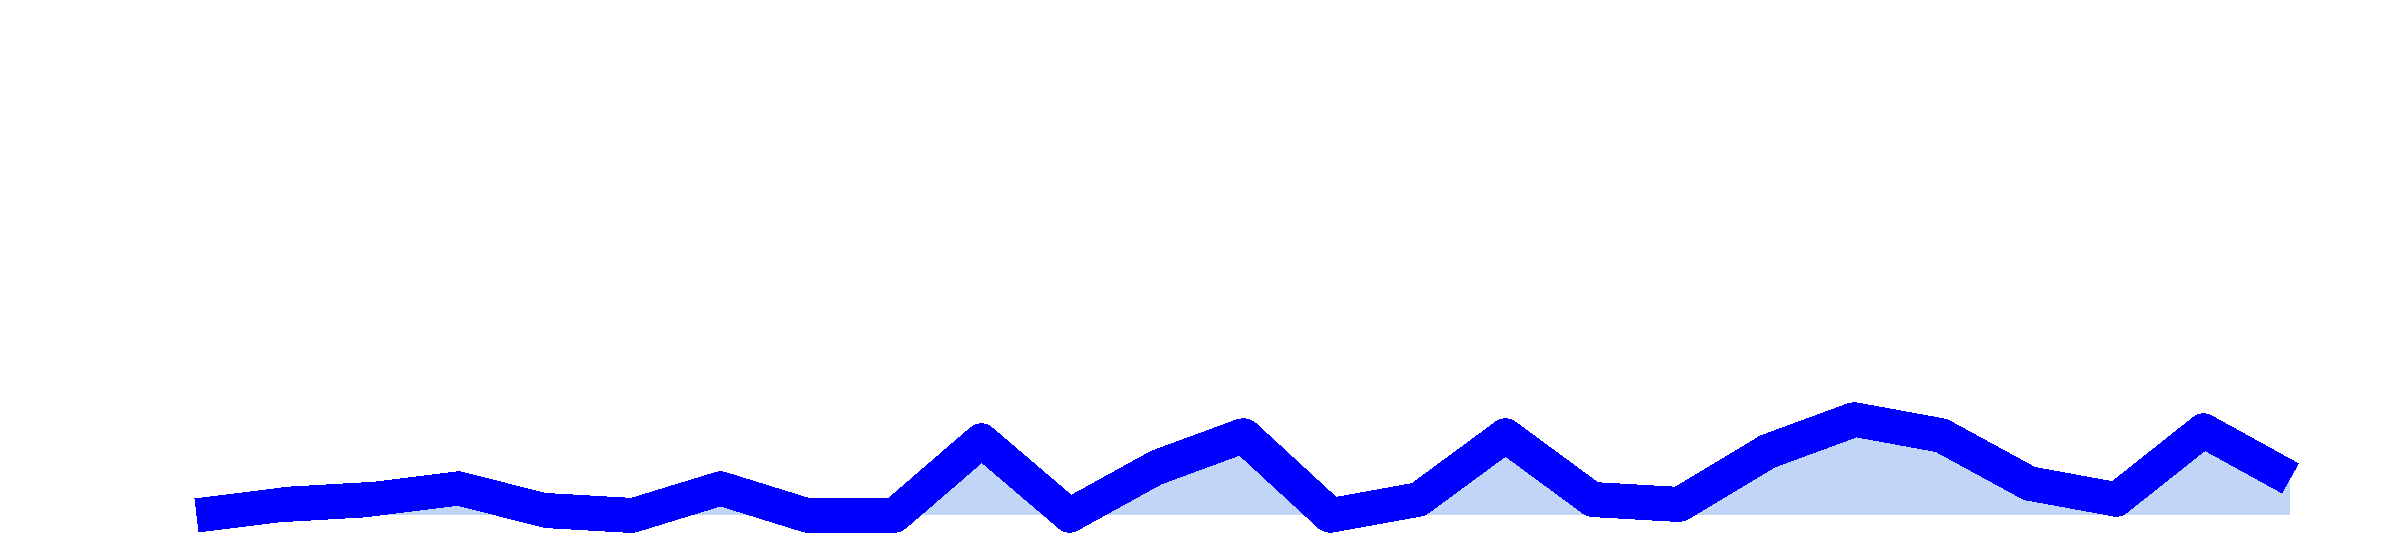
\includegraphics[width=2cm]{fig23.png}} & 2 & 0 & 27 & 29 & 543 & 63 & 63 & 63 & 63 & 63 & 63 & 0.63 & 540 & 528\\
24 & 194 & 48 & \raisebox{.12\height} {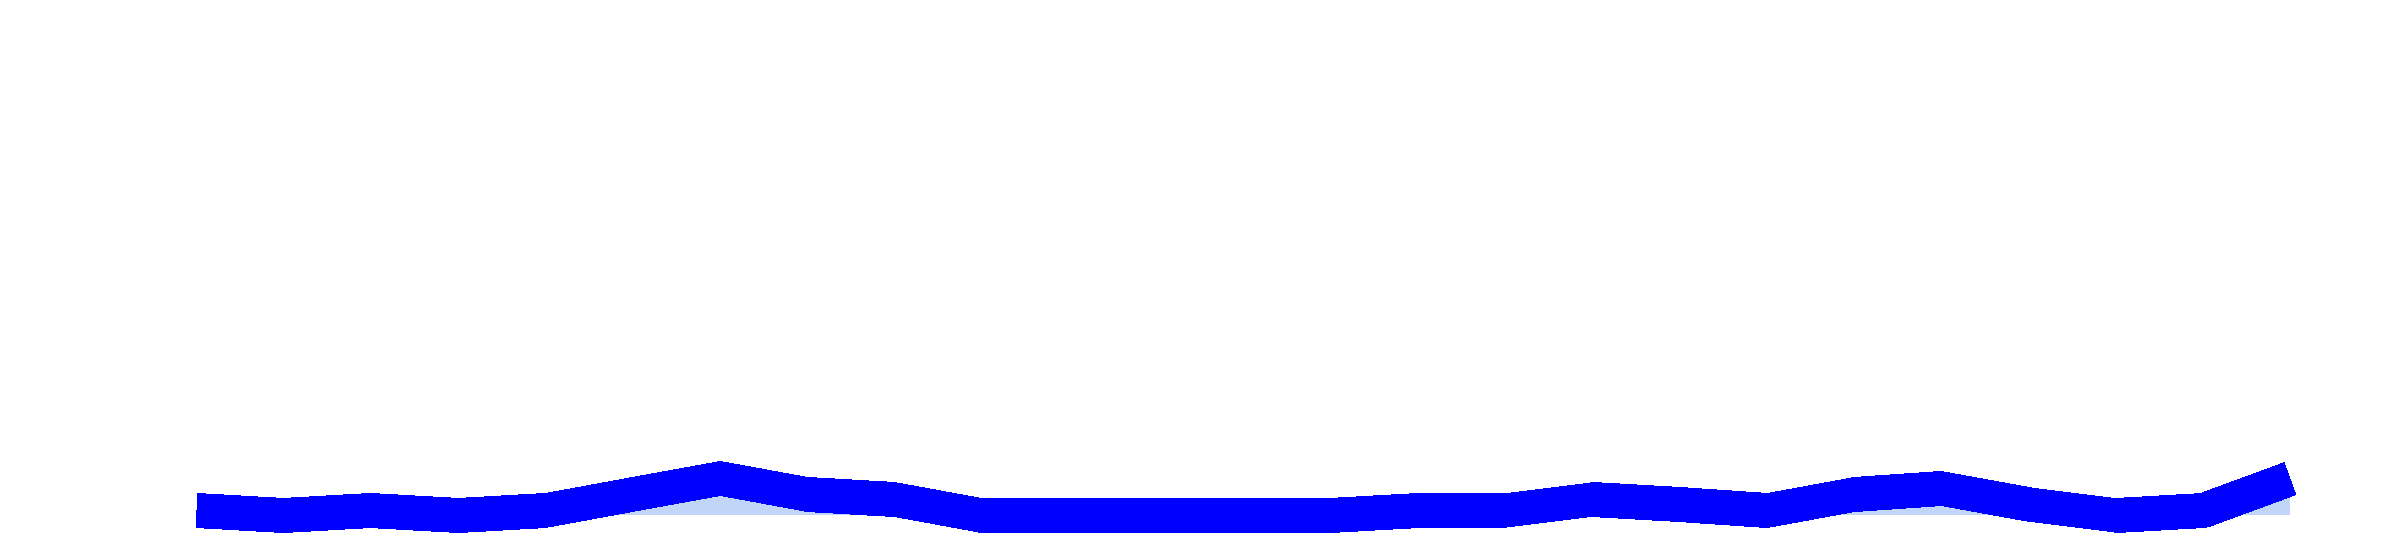
\includegraphics[width=2cm]{fig24.png}} & 0 & 0 & 20 & 20 & 694 & 28 & 28 & 28 & 28 & 28 & 28 & 0.00 & 0 & 700\\
25 & 219 & 71 & \raisebox{.12\height} {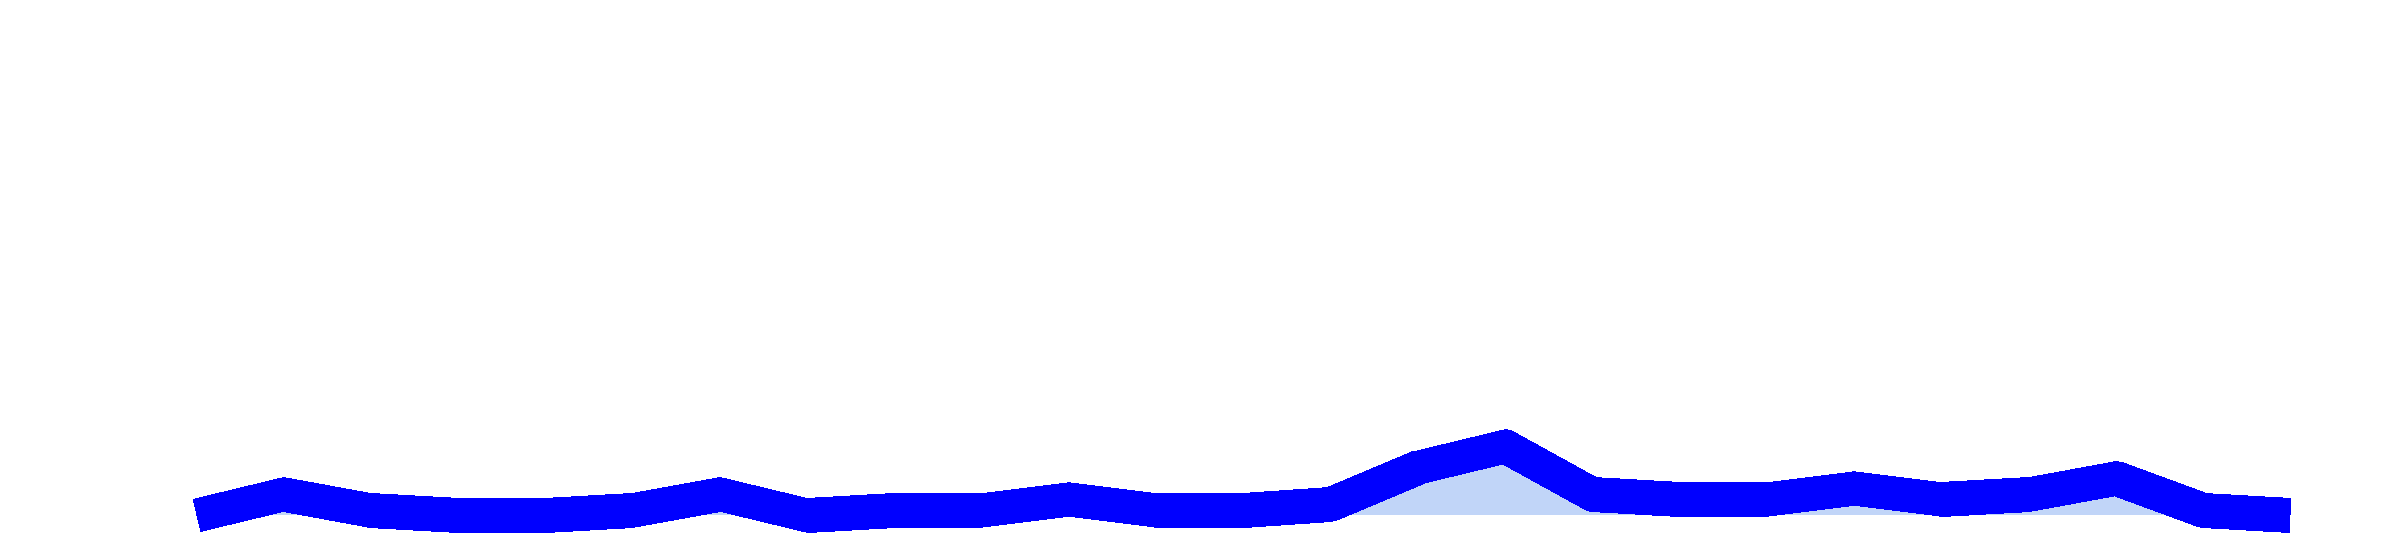
\includegraphics[width=2cm]{fig25.png}} & 0 & 0 & 26 & 26 & 675 & 40 & 40 & 40 & 40 & 40 & 40 & 0.73 & 606 & 703\\
\color{yellow}{ 26 } & 3 & 1 & \raisebox{.12\height} {
\includegraphics[width=2cm]{fig26.png}} & 0 & 0 & 0 & 0 &  & 0 & 0 & 0 &  & 0 & 0 & 0.00 & 0 & 0\\
27 & 482 & 184 & \raisebox{.12\height} {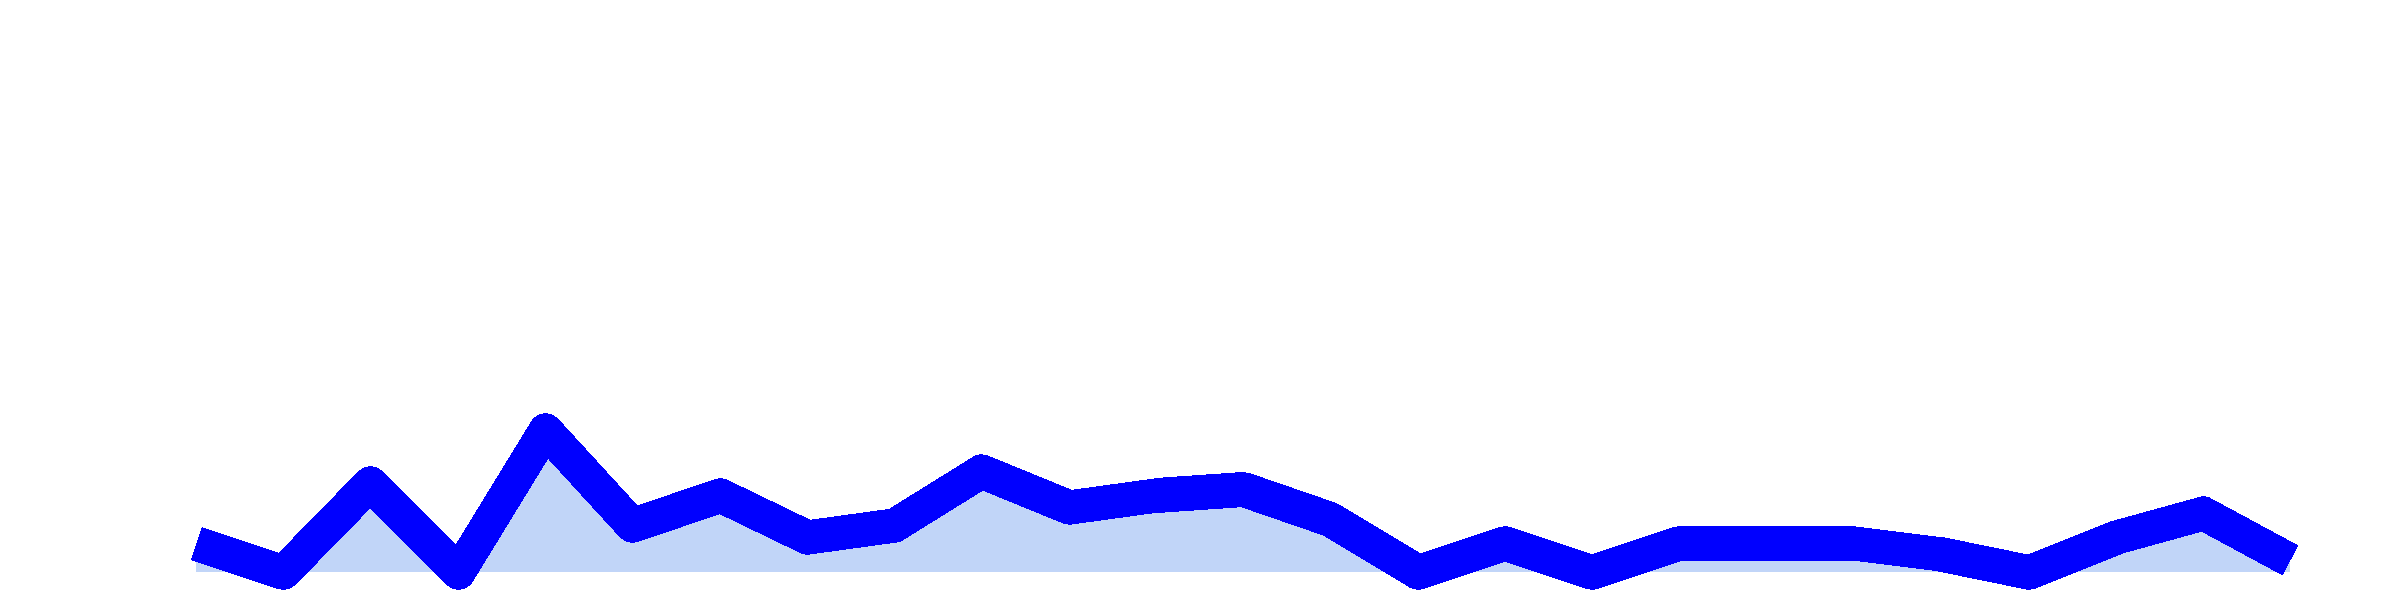
\includegraphics[width=2cm]{fig27.png}} & 1 & 0 & 61 & 62 & 620 & 56 & 56 & 56 & 56 & 56 & 56 & 0.68 & 579 & 632\\
28 & 371 & 160 & \raisebox{.12\height} {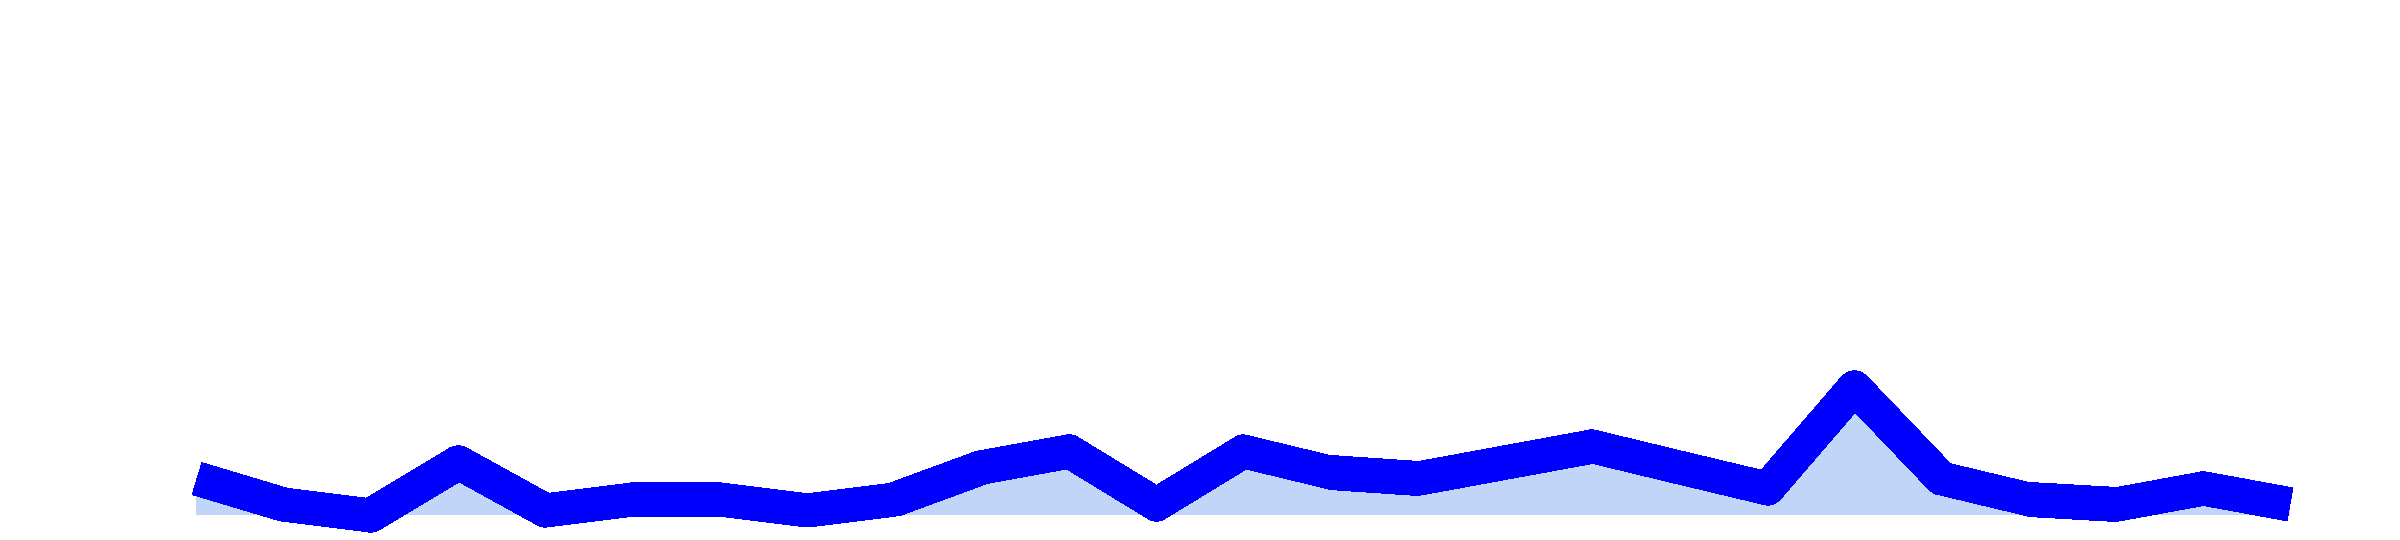
\includegraphics[width=2cm]{fig28.png}} & 0 & 0 & 61 & 61 & 606 & 56 & 56 & 56 & 56 & 56 & 56 & 0.54 & 567 & 612\\
29 & 234 & 84 & \raisebox{.12\height} {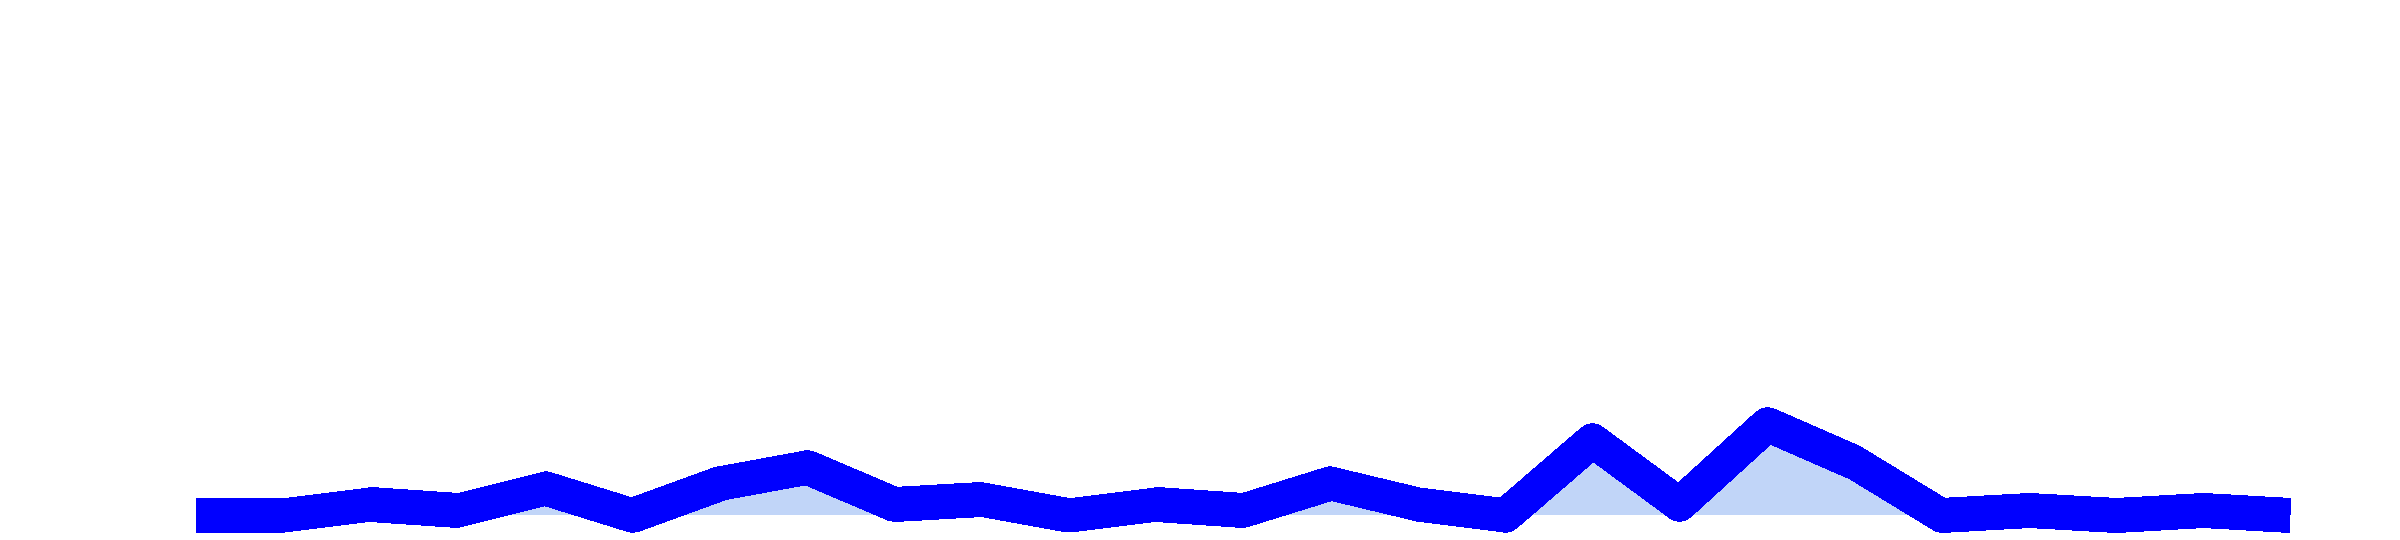
\includegraphics[width=2cm]{fig29.png}} & 0 & 0 & 11 & 11 & 621 & 62 & 62 & 62 & 62 & 62 & 62 & 0.26 & 589 & 626\\
30 & 56 & 21 & \raisebox{.12\height} {\includegraphics[width=2cm]{fig30.png}} & 0 & 0 & 7 & 7 & 612 & 14 & 14 & 14 & 14 & 14 & 14 & 0.43 & 590 & 651\\
31 & 195 & 93 & \raisebox{.12\height} {\includegraphics[width=2cm]{fig31.png}} & 1 & 0 & 27 & 28 & 585 & 46 & 46 & 45 & 46 & 45 & 46 & 0.78 & 568 & 649\\
32 & 422 & 260 & \raisebox{.12\height} {\includegraphics[width=2cm]{fig32.png}} & 0 & 0 & 103 & 103 & 534 & 47 & 47 & 47 & 47 & 47 & 47 & 0.53 & 512 & 557\\
33 & 146 & 56 & \raisebox{.12\height} {\includegraphics[width=2cm]{fig33.png}} & 1 & 0 & 20 & 21 & 629 & 35 & 35 & 35 & 35 & 35 & 35 & 0.26 & 584 & 629\\
34 & 180 & 74 & \raisebox{.12\height} {\includegraphics[width=2cm]{fig34.png}} & 0 & 0 & 16 & 16 & 599 & 48 & 48 & 48 & 48 & 48 & 48 & 0.63 & 572 & 664\\
35 & 415 & 195 & \raisebox{.12\height} {\includegraphics[width=2cm]{fig35.png}} & 0 & 0 & 61 & 61 & 563 & 54 & 54 & 50 & 54 & 50 & 54 & 0.59 & 553 & 641\\
36 & 291 & 101 & \raisebox{.12\height} {\includegraphics[width=2cm]{fig36.png}} & 0 & 0 & 26 & 26 & 627 & 41 & 41 & 41 & 41 & 41 & 41 & 0.68 & 624 & 665\\
37 & 339 & 126 & \raisebox{.12\height} {\includegraphics[width=2cm]{fig37.png}} & 0 & 0 & 43 & 43 & 620 & 53 & 53 & 53 & 53 & 53 & 53 & 0.40 & 571 & 662\\
38 & 593 & 297 & \raisebox{.12\height} {\includegraphics[width=2cm]{fig38.png}} & 0 & 0 & 113 & 113 & 576 & 60 & 60 & 60 & 60 & 60 & 60 & 0.73 & 548 & 618\\
39 & 69 & 18 & \raisebox{.12\height} {\includegraphics[width=2cm]{fig39.png}} & 0 & 0 & 7 & 7 & 683 & 11 & 11 & 11 & 11 & 11 & 11 & 0.09 & 697 & 710\\
40 & 387 & 149 & \raisebox{.12\height} {\includegraphics[width=2cm]{fig40.png}} & 0 & 0 & 75 & 75 & 601 & 51 & 51 & 51 & 51 & 51 & 51 & 0.55 & 592 & 676\\
41 & 774 & 300 & \raisebox{.12\height} {\includegraphics[width=2cm]{fig41.png}} & 0 & 0 & 124 & 123 & 617 & 54 & 54 & 54 & 54 & 54 & 54 & 0.91 & 623 & 705\\
\color{magenta}{ 43 } & 1 & 1 & \raisebox{.12\height} {\includegraphics[width=2cm]{fig43.png}} & 0 & 0 & 0 & 0 &  & 1 & 1 & 1 & 1 & 0 & 1 & 1.00 & 453 & 0\\
44 & 351 & 92 & \raisebox{.12\height} {\includegraphics[width=2cm]{fig44.png}} & 0 & 0 & 26 & 26 & 695 & 57 & 57 & 57 & 57 & 0 & 57 & 0.28 & 646 & 697\\
45 & 657 & 251 & \raisebox{.12\height} {\includegraphics[width=2cm]{fig45.png}} & 1 & 0 & 97 & 97 & 599 & 49 & 49 & 49 & 49 & 49 & 49 & 0.71 & 588 & 602\\
46 & 325 & 107 & \raisebox{.12\height} {\includegraphics[width=2cm]{fig46.png}} & 0 & 0 & 34 & 34 & 642 & 51 & 51 & 50 & 51 & 51 & 51 & 0.22 & 642 & 663\\
47 & 256 & 87 & \raisebox{.12\height} {\includegraphics[width=2cm]{fig47.png}} & 1 & 0 & 19 & 20 & 601 & 53 & 53 & 53 & 53 & 53 & 53 & 0.38 & 631 & 660\\
48 & 355 & 140 & \raisebox{.12\height} {\includegraphics[width=2cm]{fig48.png}} & 1 & 0 & 53 & 54 & 601 & 55 & 55 & 55 & 55 & 55 & 55 & 0.58 & 583 & 620\\
49 & 315 & 103 & \raisebox{.12\height} {\includegraphics[width=2cm]{fig49.png}} & 0 & 0 & 17 & 17 & 637 & 61 & 61 & 61 & 61 & 0 & 61 & 0.18 & 572 & 635\\
50 & 453 & 127 & \raisebox{.12\height} {\includegraphics[width=2cm]{fig50.png}} & 0 & 0 & 39 & 39 & 659 & 47 & 47 & 47 & 47 & 47 & 47 & 0.15 & 636 & 677\\
51 & 29 & 11 & \raisebox{.12\height} {\includegraphics[width=2cm]{fig51.png}} & 0 & 0 & 1 & 1 & 559 & 8 & 8 & 8 & 8 & 8 & 8 & 0.38 & 617 & 625\\
52 & 592 & 207 & \raisebox{.12\height} {\includegraphics[width=2cm]{fig52.png}} & 0 & 0 & 84 & 84 & 633 & 51 & 51 & 51 & 51 & 51 & 51 & 0.33 & 599 & 661\\
53 & 153 & 29 & \raisebox{.12\height} {\includegraphics[width=2cm]{fig53.png}} & 0 & 0 & 9 & 9 & 801 & 20 & 20 & 20 & 20 & 20 & 20 & 0.20 & 685 & 747\\
54 & 336 & 101 & \raisebox{.12\height} {\includegraphics[width=2cm]{fig54.png}} & 0 & 0 & 30 & 29 & 664 & 45 & 48 & 48 & 48 & 48 & 48 & 0.25 & 606 & 666\\
55 & 591 & 297 & \raisebox{.12\height} {\includegraphics[width=2cm]{fig55.png}} & 0 & 0 & 137 & 137 & 562 & 53 & 53 & 53 & 53 & 53 & 53 & 0.85 & 555 & 572\\
56 & 213 & 54 & \raisebox{.12\height} {\includegraphics[width=2cm]{fig56.png}} & 1 & 0 & 15 & 16 & 707 & 38 & 38 & 38 & 38 & 38 & 38 & 0.05 & 664 & 705\\
57 & 1181 & 654 & \raisebox{.12\height} {\includegraphics[width=2cm]{fig57.png}} & 2 & 0 & 273 & 275 & 544 & 57 & 57 & 57 & 57 & 57 & 57 & 0.56 & 557 & 531\\
58 & 641 & 222 & \raisebox{.12\height} {\includegraphics[width=2cm]{fig58.png}} & 1 & 0 & 65 & 66 & 636 & 52 & 52 & 52 & 52 & 52 & 52 & 0.33 & 617 & 640\\
59 & 131 & 41 & \raisebox{.12\height} {\includegraphics[width=2cm]{fig59.png}} & 1 & 0 & 19 & 20 & 697 & 20 & 20 & 20 & 20 & 0 & 20 & 0.20 & 639 & 620\\
60 & 151 & 54 & \raisebox{.12\height} {\includegraphics[width=2cm]{fig60.png}} & 0 & 0 & 16 & 16 & 659 & 34 & 34 & 34 & 34 & 34 & 34 & 0.15 & 590 & 632\\
61 & 668 & 432 & \raisebox{.12\height} {\includegraphics[width=2cm]{fig61.png}} & 1 & 0 & 114 & 115 & 536 & 59 & 59 & 59 & 59 & 59 & 59 & 0.59 & 516 & 541\\
62 & 710 & 373 & \raisebox{.12\height} {\includegraphics[width=2cm]{fig62.png}} & 0 & 0 & 132 & 132 & 557 & 60 & 60 & 60 & 60 & 60 & 60 & 0.77 & 549 & 604\\
63 & 305 & 115 & \raisebox{.12\height} {\includegraphics[width=2cm]{fig63.png}} & 2 & 0 & 41 & 43 & 634 & 49 & 49 & 48 & 49 & 48 & 49 & 0.22 & 598 & 631\\
64 & 42 & 10 & \raisebox{.12\height} {\includegraphics[width=2cm]{fig64.png}} & 0 & 0 & 2 & 2 & 767 & 7 & 7 & 7 & 7 & 7 & 7 & 0.00 & 0 & 700\\
65 & 953 & 482 & \raisebox{.12\height} {\includegraphics[width=2cm]{fig65.png}} & 1 & 0 & 151 & 151 & 568 & 61 & 61 & 61 & 61 & 61 & 61 & 0.77 & 564 & 587\\
66 & 924 & 401 & \raisebox{.12\height} {\includegraphics[width=2cm]{fig66.png}} & 1 & 0 & 146 & 146 & 586 & 57 & 57 & 57 & 57 & 57 & 57 & 0.51 & 582 & 631\\
67 & 531 & 155 & \raisebox{.12\height} {\includegraphics[width=2cm]{fig67.png}} & 0 & 0 & 50 & 50 & 672 & 50 & 50 & 50 & 50 & 50 & 50 & 0.32 & 617 & 667\\
68 & 360 & 87 & \raisebox{.12\height} {\includegraphics[width=2cm]{fig68.png}} & 1 & 0 & 40 & 41 & 707 & 39 & 39 & 39 & 39 & 39 & 39 & 0.15 & 609 & 704\\
69 & 22 & 4 & \raisebox{.12\height} {\includegraphics[width=2cm]{fig69.png}} & 0 & 0 & 3 & 3 & 761 & 2 & 2 & 2 & 2 & 2 & 2 & 0.50 & 558 & 778\\
70 & 91 & 24 & \raisebox{.12\height} {\includegraphics[width=2cm]{fig70.png}} & 0 & 0 & 9 & 9 & 670 & 15 & 15 & 15 & 15 & 15 & 15 & 0.13 & 686 & 707\\
71 & 246 & 86 & \raisebox{.12\height} {\includegraphics[width=2cm]{fig71.png}} & 0 & 0 & 24 & 24 & 644 & 48 & 48 & 48 & 48 & 48 & 48 & 0.33 & 619 & 661\\
72 & 101 & 21 & \raisebox{.12\height} {\includegraphics[width=2cm]{fig72.png}} & 0 & 0 & 6 & 6 & 725 & 11 & 11 & 11 & 11 & 11 & 11 & 0.09 & 710 & 759\\
73 & 391 & 132 & \raisebox{.12\height} {\includegraphics[width=2cm]{fig73.png}} & 1 & 0 & 30 & 31 & 646 & 56 & 56 & 56 & 56 & 56 & 56 & 0.68 & 617 & 707\\
74 & 279 & 62 & \raisebox{.12\height} {\includegraphics[width=2cm]{fig74.png}} & 0 & 0 & 24 & 23 & 682 & 38 & 38 & 38 & 38 & 38 & 38 & 0.18 & 672 & 752\\
75 & 203 & 55 & \raisebox{.12\height} {\includegraphics[width=2cm]{fig75.png}} & 0 & 0 & 18 & 18 & 688 & 34 & 34 & 34 & 34 & 34 & 34 & 0.35 & 621 & 690\\
76 & 403 & 160 & \raisebox{.12\height} {\includegraphics[width=2cm]{fig76.png}} & 1 & 0 & 42 & 43 & 611 & 47 & 47 & 47 & 47 & 47 & 47 & 0.38 & 581 & 660\\
77 & 16 & 3 & \raisebox{.12\height} {\includegraphics[width=2cm]{fig77.png}} & 0 & 0 & 0 & 0 &  & 3 & 3 & 3 & 3 & 3 & 3 & 0.00 & 0 & 799\\
78 & 1100 & 333 & \raisebox{.12\height} {\includegraphics[width=2cm]{fig78.png}} & 2 & 0 & 123 & 125 & 651 & 55 & 55 & 55 & 55 & 55 & 55 & 0.47 & 629 & 693\\
79 & 382 & 120 & \raisebox{.12\height} {\includegraphics[width=2cm]{fig79.png}} & 1 & 0 & 35 & 36 & 637 & 46 & 47 & 47 & 47 & 47 & 47 & 0.26 & 631 & 675\\
80 & 14 & 4 & \raisebox{.12\height} {\includegraphics[width=2cm]{fig80.png}} & 0 & 0 & 0 & 0 &  & 4 & 4 & 4 & 4 & 4 & 4 & 0.25 & 642 & 685\\
81 & 628 & 192 & \raisebox{.12\height} {\includegraphics[width=2cm]{fig81.png}} & 1 & 0 & 82 & 83 & 646 & 53 & 54 & 54 & 54 & 54 & 54 & 0.52 & 616 & 659\\
82 & 277 & 100 & \raisebox{.12\height} {\includegraphics[width=2cm]{fig82.png}} & 2 & 1 & 36 & 38 & 619 & 53 & 53 & 53 & 53 & 53 & 53 & 0.79 & 613 & 621\\
83 & 679 & 194 & \raisebox{.12\height} {\includegraphics[width=2cm]{fig83.png}} & 0 & 0 & 76 & 76 & 661 & 58 & 58 & 58 & 58 & 58 & 58 & 0.43 & 639 & 681\\
84 & 615 & 219 & \raisebox{.12\height} {\includegraphics[width=2cm]{fig84.png}} & 3 & 0 & 54 & 57 & 625 & 58 & 58 & 58 & 58 & 58 & 58 & 0.40 & 604 & 648\\
85 & 72 & 18 & \raisebox{.12\height} {\includegraphics[width=2cm]{fig85.png}} & 0 & 0 & 5 & 5 & 680 & 6 & 6 & 6 & 6 & 6 & 6 & 0.00 & 0 & 706\\
86 & 115 & 25 & \raisebox{.12\height} {\includegraphics[width=2cm]{fig86.png}} & 0 & 0 & 7 & 7 & 699 & 18 & 18 & 18 & 18 & 18 & 18 & 0.28 & 716 & 693\\
87 & 404 & 122 & \raisebox{.12\height} {\includegraphics[width=2cm]{fig87.png}} & 0 & 0 & 55 & 54 & 640 & 55 & 55 & 55 & 55 & 55 & 55 & 0.22 & 630 & 674\\
88 & 100 & 21 & \raisebox{.12\height} {\includegraphics[width=2cm]{fig88.png}} & 0 & 0 & 3 & 3 & 692 & 18 & 18 & 18 & 18 & 18 & 18 & 0.22 & 697 & 796\\
89 & 338 & 171 & \raisebox{.12\height} {\includegraphics[width=2cm]{fig89.png}} & 1 & 0 & 73 & 74 & 578 & 38 & 38 & 38 & 38 & 38 & 38 & 0.87 & 553 & 692\\
90 & 26 & 7 & \raisebox{.12\height} {\includegraphics[width=2cm]{fig90.png}} & 0 & 0 & 7 & 7 & 721 & 0 & 0 & 0 & 0 & 0 & 0 & 0.00 & 0 & 0\\
91 & 194 & 92 & \raisebox{.12\height} {\includegraphics[width=2cm]{fig91.png}} & 1 & 0 & 37 & 38 & 569 & 45 & 45 & 45 & 45 & 45 & 45 & 0.80 & 554 & 624\\
92 & 29 & 8 & \raisebox{.12\height} {\includegraphics[width=2cm]{fig92.png}} & 0 & 0 & 4 & 4 & 698 & 4 & 4 & 4 & 4 & 4 & 4 & 0.25 & 648 & 718\\
93 & 269 & 67 & \raisebox{.12\height} {\includegraphics[width=2cm]{fig93.png}} & 1 & 0 & 25 & 26 & 696 & 41 & 41 & 41 & 41 & 41 & 41 & 0.12 & 657 & 710\\
94 & 139 & 53 & \raisebox{.12\height} {\includegraphics[width=2cm]{fig94.png}} & 1 & 0 & 29 & 30 & 638 & 23 & 23 & 23 & 23 & 23 & 23 & 0.78 & 641 & 688\\
95 & 116 & 40 & \raisebox{.12\height} {\includegraphics[width=2cm]{fig95.png}} & 1 & 0 & 12 & 13 & 650 & 27 & 27 & 27 & 27 & 27 & 27 & 0.41 & 621 & 667\\
96 & 12 & 4 & \raisebox{.12\height} {\includegraphics[width=2cm]{fig96.png}} & 0 & 0 & 2 & 2 & 655 & 2 & 2 & 2 & 2 & 2 & 2 & 0.00 & 0 & 653\\
97 & 249 & 122 & \raisebox{.12\height} {\includegraphics[width=2cm]{fig97.png}} & 0 & 0 & 50 & 50 & 564 & 52 & 52 & 52 & 52 & 52 & 52 & 0.79 & 556 & 648\\
98 & 139 & 58 & \raisebox{.12\height} {\includegraphics[width=2cm]{fig98.png}} & 1 & 0 & 30 & 31 & 608 & 27 & 27 & 27 & 27 & 27 & 27 & 0.70 & 583 & 611\\
99 & 188 & 72 & \raisebox{.12\height} {\includegraphics[width=2cm]{fig99.png}} & 0 & 0 & 22 & 22 & 625 & 38 & 38 & 38 & 38 & 38 & 38 & 0.71 & 578 & 610\\
100 & 230 & 62 & \raisebox{.12\height} {\includegraphics[width=2cm]{fig100.png}} & 0 & 0 & 15 & 15 & 706 & 41 & 41 & 41 & 41 & 41 & 41 & 0.17 & 593 & 706\\
101 & 160 & 42 & \raisebox{.12\height} {\includegraphics[width=2cm]{fig101.png}} & 0 & 0 & 17 & 17 & 671 & 24 & 24 & 24 & 24 & 24 & 24 & 0.21 & 665 & 703\\
102 & 452 & 152 & \raisebox{.12\height} {\includegraphics[width=2cm]{fig102.png}} & 0 & 0 & 52 & 52 & 645 & 56 & 56 & 56 & 56 & 56 & 56 & 0.66 & 602 & 674\\
103 & 1306 & 435 & \raisebox{.12\height} {\includegraphics[width=2cm]{fig103.png}} & 0 & 0 & 168 & 168 & 627 & 58 & 58 & 58 & 58 & 58 & 58 & 0.41 & 611 & 674\\
104 & 1315 & 533 & \raisebox{.12\height} {\includegraphics[width=2cm]{fig104.png}} & 1 & 0 & 203 & 202 & 598 & 41 & 41 & 41 & 41 & 41 & 41 & 0.61 & 583 & 616\\
105 & 359 & 112 & \raisebox{.12\height} {\includegraphics[width=2cm]{fig105.png}} & 0 & 0 & 45 & 45 & 665 & 53 & 53 & 53 & 53 & 53 & 53 & 0.45 & 640 & 694\\
106 & 480 & 152 & \raisebox{.12\height} {\includegraphics[width=2cm]{fig106.png}} & 0 & 0 & 57 & 57 & 648 & 51 & 51 & 51 & 51 & 49 & 51 & 0.53 & 610 & 698\\
107 & 252 & 72 & \raisebox{.12\height} {\includegraphics[width=2cm]{fig107.png}} & 0 & 0 & 33 & 32 & 669 & 39 & 39 & 39 & 39 & 39 & 39 & 0.41 & 677 & 719\\
108 & 281 & 89 & \raisebox{.12\height} {\includegraphics[width=2cm]{fig108.png}} & 0 & 0 & 38 & 38 & 653 & 50 & 50 & 50 & 50 & 50 & 50 & 0.58 & 593 & 669\\
109 & 684 & 211 & \raisebox{.12\height} {\includegraphics[width=2cm]{fig109.png}} & 0 & 0 & 72 & 71 & 673 & 51 & 50 & 50 & 51 & 51 & 51 & 0.58 & 652 & 711\\
110 & 746 & 217 & \raisebox{.12\height} {\includegraphics[width=2cm]{fig110.png}} & 1 & 0 & 72 & 73 & 644 & 54 & 54 & 54 & 54 & 54 & 54 & 0.63 & 619 & 689\\
111 & 447 & 118 & \raisebox{.12\height} {\includegraphics[width=2cm]{fig111.png}} & 0 & 0 & 36 & 36 & 659 & 42 & 42 & 42 & 42 & 42 & 42 & 0.50 & 638 & 678\\
112 & 152 & 30 & \raisebox{.12\height} {\includegraphics[width=2cm]{fig112.png}} & 0 & 0 & 11 & 11 & 722 & 17 & 17 & 17 & 17 & 17 & 17 & 0.24 & 714 & 760\\
113 & 1228 & 586 & \raisebox{.12\height} {\includegraphics[width=2cm]{fig113.png}} & 0 & 0 & 186 & 186 & 572 & 62 & 62 & 62 & 62 & 62 & 62 & 0.31 & 541 & 596\\
114 & 813 & 546 & \raisebox{.12\height} {\includegraphics[width=2cm]{fig114.png}} & 0 & 0 & 177 & 177 & 523 & 61 & 61 & 61 & 61 & 61 & 61 & 0.34 & 502 & 541\\
115 & 606 & 328 & \raisebox{.12\height} {\includegraphics[width=2cm]{fig115.png}} & 0 & 0 & 118 & 118 & 537 & 55 & 55 & 55 & 55 & 55 & 55 & 0.44 & 533 & 553\\
\color{green}{ 116 } & 47 & 27 & \raisebox{.12\height} {\includegraphics[width=2cm]{fig116.png}} & 0 & 0 & 12 & 12 & 529 & 15 & 15 & 15 & 15 & 15 & 15 & 0.27 & 563 & 550\\
\color{green}{ 117 } & 496 & 284 & \raisebox{.12\height} {\includegraphics[width=2cm]{fig117.png}} & 1 & 0 & 101 & 102 & 547 & 66 & 66 & 66 & 66 & 66 & 66 & 0.36 & 525 & 538\\
\color{green}{ 118 } & 603 & 276 & \raisebox{.12\height} {\includegraphics[width=2cm]{fig118.png}} & 1 & 0 & 116 & 117 & 581 & 52 & 52 & 52 & 52 & 52 & 52 & 0.42 & 561 & 615\\
\color{green}{ 119 } & 1234 & 529 & \raisebox{.12\height} {\includegraphics[width=2cm]{fig119.png}} & 1 & 0 & 300 & 299 & 599 & 56 & 57 & 57 & 57 & 57 & 57 & 0.37 & 576 & 613\\
\color{green}{ 120 } & 1690 & 580 & \raisebox{.12\height} {\includegraphics[width=2cm]{fig120.png}} & 2 & 0 & 237 & 239 & 630 & 57 & 57 & 57 & 57 & 57 & 57 & 0.18 & 572 & 633\\
\color{green}{ 121 } & 854 & 398 & \raisebox{.12\height} {\includegraphics[width=2cm]{fig121.png}} & 2 & 0 & 144 & 146 & 582 & 51 & 51 & 51 & 51 & 51 & 51 & 0.33 & 539 & 593\\
\color{green}{ 122 } & 713 & 355 & \raisebox{.12\height} {\includegraphics[width=2cm]{fig122.png}} & 8 & 0 & 147 & 155 & 578 & 53 & 53 & 53 & 53 & 53 & 53 & 0.42 & 556 & 596\\
\color{green}{ 123 } & 1069 & 436 & \raisebox{.12\height} {\includegraphics[width=2cm]{fig123.png}} & 3 & 0 & 178 & 181 & 607 & 60 & 60 & 60 & 60 & 60 & 60 & 0.18 & 570 & 626\\
\color{green}{ 124 } & 1075 & 487 & \raisebox{.12\height} {\includegraphics[width=2cm]{fig124.png}} & 13 & 0 & 217 & 230 & 585 & 57 & 57 & 57 & 57 & 57 & 57 & 0.35 & 576 & 609\\
\color{green}{ 125 } & 852 & 409 & \raisebox{.12\height} {\includegraphics[width=2cm]{fig125.png}} & 12 & 0 & 212 & 223 & 584 & 54 & 54 & 54 & 54 & 54 & 54 & 0.46 & 548 & 607\\
\color{green}{ 126 } & 1288 & 445 & \raisebox{.12\height} {\includegraphics[width=2cm]{fig126.png}} & 14 & 0 & 186 & 200 & 636 & 44 & 44 & 44 & 44 & 44 & 44 & 0.25 & 598 & 635\\
\color{green}{ 127 } & 554 & 193 & \raisebox{.12\height} {\includegraphics[width=2cm]{fig127.png}} & 1 & 0 & 117 & 118 & 628 & 49 & 49 & 49 & 49 & 49 & 49 & 0.24 & 604 & 644\\
\color{green}{ 128 } & 1115 & 405 & \raisebox{.12\height} {\includegraphics[width=2cm]{fig128.png}} & 19 & 0 & 187 & 204 & 622 & 52 & 52 & 52 & 52 & 52 & 52 & 0.33 & 594 & 667\\
\color{green}{ 129 } & 929 & 335 & \raisebox{.12\height} {\includegraphics[width=2cm]{fig129.png}} & 5 & 0 & 177 & 182 & 631 & 69 & 69 & 68 & 69 & 68 & 69 & 0.38 & 588 & 625\\
\color{green}{ 130 } & 1282 & 488 & \raisebox{.12\height} {\includegraphics[width=2cm]{fig130.png}} & 15 & 0 & 217 & 231 & 607 & 58 & 58 & 58 & 58 & 58 & 58 & 0.41 & 575 & 658\\
\color{green}{ 131 } & 157 & 78 & \raisebox{.12\height} {\includegraphics[width=2cm]{fig131.png}} & 0 & 0 & 39 & 39 & 576 & 39 & 39 & 39 & 39 & 39 & 39 & 0.28 & 543 & 590\\
\color{green}{ 132 } & 228 & 111 & \raisebox{.12\height} {\includegraphics[width=2cm]{fig132.png}} & 0 & 0 & 22 & 22 & 571 & 42 & 42 & 42 & 42 & 42 & 42 & 0.26 & 515 & 580\\
\color{green}{ 133 } & 417 & 165 & \raisebox{.12\height} {\includegraphics[width=2cm]{fig133.png}} & 4 & 0 & 103 & 107 & 607 & 45 & 45 & 45 & 45 & 45 & 45 & 0.27 & 558 & 623\\
\color{green}{ 134 } & 446 & 159 & \raisebox{.12\height} {\includegraphics[width=2cm]{fig134.png}} & 0 & 0 & 80 & 80 & 621 & 42 & 42 & 42 & 42 & 42 & 42 & 0.33 & 582 & 637\\
\color{green}{ 135 } & 126 & 53 & \raisebox{.12\height} {\includegraphics[width=2cm]{fig135.png}} & 1 & 0 & 30 & 31 & 593 & 21 & 21 & 21 & 21 & 21 & 21 & 0.19 & 546 & 622\\
\midrule
\textbf{Total} & \textbf{57178} & \textbf{23060} & \textbf{\raisebox{.12\height} {\includegraphics[width=2cm]{figTotal.png}}} & \textbf{151} & \textbf{1} & \textbf{8574} & \textbf{8708} & \textbf{} & \textbf{5677} & \textbf{5682} & \textbf{5674} & \textbf{5683} & \textbf{5535} & \textbf{5683} & \textbf{} & \textbf{} & \textbf{}\\*
\end{longtable}
\endgroup{}
\end{landscape}
\clearpage

\end{appendices}

\hypertarget{refs}{}
\leavevmode\hypertarget{ref-Cox2011}{}%
Cox, S.P., Kronlund, A.R., and Lacko, L.C. 2011. Management procedures for the multi-gear sablefish (\emph{Anoplopoma fimbria}) fishery in British Columbia, Canada. DFO Can. Sci. Advis. Sec. Res. Doc. 2011/063: viii + 45 p.

\leavevmode\hypertarget{ref-DFO2020}{}%
DFO. 2020. Evaluating the robustness of candidate management procedures in the BC Sablefish (\emph{Anoplopoma fimbria}) fishery for 2019-2020. DFO Can. Sci. Advis. Sec. Sci. Resp. (25).

\leavevmode\hypertarget{ref-DFO2021}{}%
DFO. 2021. Evaluating the robustness of candidate management procedures in the BC Sablefish (\emph{Anoplopoma fimbria}) fishery for 2020-2021. DFO Can. Sci. Advis. Sec. Sci. Resp. (25).

\leavevmode\hypertarget{ref-Downes1997}{}%
Downes, A.J., Andrews, W.T., Smith, M.S., Saunders, M.W., and Jewsbury., G.D. 1997. Cruise details of Sablefish (\emph{Anoplopoma fimbria}) surveys conducted in B.C. waters, 1994-1995. Can. Data Rep. Fish. Aquat. Sci. 1997/1007: 106 p.

\leavevmode\hypertarget{ref-Olsen2010}{}%
Olsen, N. 2010. CA user's guide to GFBioField: The Pacific Region's at-sea data acquisition system for groundfish trawl surveys. Can. Tech. Rep. Fish.Aquat. Sci. 2010/2887: x + 76 p.

\leavevmode\hypertarget{ref-Orr2008}{}%
Orr, J.W., and Hawkins, S. 2008. Species of the rougheye rockfish complex resurrection of Sebastes melanostictus (Matsubara, 1934) and a redescription of Sebastes aleutianus (Jordan and Evermann, 1898) (Teleostei: Scorpaeniformes). Fish. Bull. 106(2): 111--134.

\leavevmode\hypertarget{ref-Smith1996}{}%
Smith, M.S., Saunders, M.W., and Andrews, W.T. 1996. Cruise details of sablefish (\emph{Anoplopoma fimbria}) surveys conducted in B.C. waters 1988-1993. Can. Tech. Rep. Fish.Aquat. Sci. 1996/976: 129 p.

\leavevmode\hypertarget{ref-Wyeth2003}{}%
Wyeth, M.R., and Kronlund, A.R. 2003. Sablefish (\emph{Anoplopoma fimbria}) research and assessment surveys conducted in British Columbia waters from 1996 through 2000. Can. Data Rep. Fish. Aquat. Sci. 2003/1116: 130 p.

\leavevmode\hypertarget{ref-Wyeth2004b}{}%
Wyeth, M.R., Kronlund, A.R., and Elfert, M. 2004a. Summary of the 2003 British Columbia Sablefish (\emph{Anoplopoma fimbria}) Research and Assessment Survey. Can. Data Rep. Fish. Aquat. Sci. 2004/1148: 68 p.

\leavevmode\hypertarget{ref-Wyeth2004a}{}%
Wyeth, M.R., Kronlund, A.R., and Elfert, M. 2004b. Summary of the 2002 British Columbia Sablefish (\emph{Anoplopoma fimbria}) Research and Assessment Survey. Can. Data Rep. Fish. Aquat. Sci. 2004/1140: 59 p.

\leavevmode\hypertarget{ref-Wyeth2006}{}%
Wyeth, M.R., Kronlund, A.R., and Elfert, M. 2006. Summary of the 2004 British Columbia Sablefish (\emph{Anoplopoma fimbria}) Research and Assessment Surveys. Can. Data Rep. Fish. Aquat. Sci. 2006/2660: 74 p.
\end{document}
